\chapter{营养与代谢综合征}

\hypertarget{text00004.htmlux5cux23mllj1}{%
\section{ 代谢综合征}\label{text00004.htmlux5cux23mllj1}}

代谢综合征(metabolic syndrome,
MS)是与各类血管的病变(心、脑、肠血管)及糖尿病的发生、发展密切相关的一组症候群。MS概念的形成和发展到目前全球统一诊断标准的提出经历了一个漫长的过程。胰岛素抵抗曾被认为是其病理生理基础,然而近年大量研究显示,胰岛素抵抗只是MS发病的一个重要环节,还有许多因素参与。因此,MS的概念和诊断标准虽较过去有了明确定义,但仍在不断完善和修订中。

\hypertarget{text00004.htmlux5cux23mllj2}{%
\subsection{代谢综合征的流行病学}\label{text00004.htmlux5cux23mllj2}}

近几十年来,随着全球经济快速发展,人们的生活方式也发生了巨大变化。每天高能量的摄入,以及静坐休闲时间明显增多(汽车和家电业的发展),使慢性代谢性疾病(肥胖病、高血压、血脂异常、糖尿病、痛风等)的发病率呈流行趋势。MS发病率又因不同种族、不同地区、不同诊断标准而有所不同。在美国,印第安人MS患病率最高,达40%以上,而非洲裔最低。在我国,MS和超重的患病率北方高于南方、城市高于农村、男性高于女性,并且有增龄效应等流行病学特征。有研究发现,在上海社区20~74岁人群中,约1/6患MS,>45岁男性及>50岁女性患病率明显增加。65~69岁达到高峰。MS的高患病率预示着心脑血管疾病发病率和死亡率的增加。随着我国人口的老龄化,MS的出现将意味着我国老年人群心脑血管疾病发生高峰的到来。

\hypertarget{text00004.htmlux5cux23mllj3}{%
\subsection{代谢综合征的诊断标准}\label{text00004.htmlux5cux23mllj3}}

MS的诊断标准如表3-1所示\footnote{*注:NCEP-ATP Ⅲ:National Cholesterol Education Program-The Adult
Treatment Panel
Ⅲ,美国国家胆固醇教育计划的成人治疗专家组Ⅲ;CDS:中国糖尿病协会;IDF:国际糖尿病协会(International
Diabetes Federation);IR:胰岛素抵抗。}。

\begin{table}[htbp]
\centering
\caption{MS诊断标准比较}
\label{tab3-1}
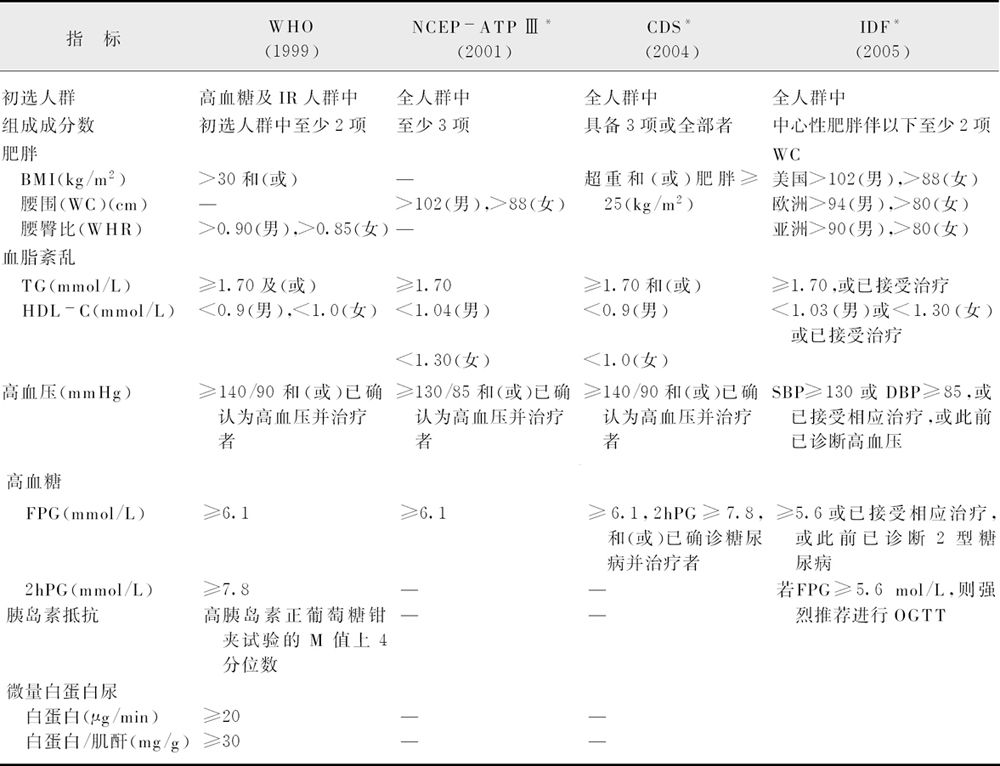
\includegraphics{./images/Image00016.jpg}
\end{table}



新近国内学者开始对WHO、ATP、CDS和IDF等MS诊断指标进行比较,如顾卫琼等研究认为,在发生MS人群中,以IDF定义下的人群发病率最高。WHO定义因其对胰岛素抵抗的要求,实用性较差,而ATP定义人群基本被IDF覆盖。体脂分布的异常(中心性肥胖,非体脂含量)加剧了代谢紊乱的发生和胰岛素抵抗的程度。IDF定义完全以腰围测量作为衡量中心性肥胖指标,并将中心性肥胖视为胰岛素抵抗的临床标志。另一方面,降低了血糖的标准,以及考虑到不同种族的差异,是较为适合的MS诊断标准,但是否能适合更多中国人群的诊断标准,仍需我们进行不断的探索和实践。

\hypertarget{text00004.htmlux5cux23mllj4}{%
\subsection{代谢综合征的病因及病理生理机制}\label{text00004.htmlux5cux23mllj4}}

MS病因及病理生理机制非常复杂。这主要是由于:①MS的定义尚未完全统一;②MS一般由多重因素引起;③其发病表现在不同个体中有所不同。

(一)代谢综合征的病因

{1.脂质损伤学说}
 脂质损伤学说实质上包含两个假说:一个是McGarry提出的糖尿病的脂毒性假说;第二个是Unger提出的MS的脂质堆积和溢出假说。

(1)糖尿病的脂毒性假说:该假说认为在生理条件下脂肪分解产生游离脂肪酸(free
fatty acid,
FFA)释放进入血液循环,当血中FFA水平超过各组织对其的分解和氧化能力时,FFA则将以三酰甘油(TG)的形式在非脂肪组织中沉积,从而造成该组织的损伤。如在胰岛素靶组织(如肝脏、肌肉)中过度沉积,将导致胰岛素抵抗(insulin
resistance,
IR);如异位沉积在胰岛B细胞,将导致胰岛功能损伤、胰岛素分泌障碍,最终导致糖尿病的发生和发展。

(2)脂质堆积和溢出假说:肥胖时由于瘦素(leptin)抵抗引起机体脂质分泌异常,进而由胰岛素刺激的脂肪酶活性增高、脂肪合成增加及脂质异位堆积和溢出,产生葡萄糖代谢的胰岛素抵抗,最终导致MS的发生。

这两种学说的区别在于,脂质堆积和溢出学说把瘦素抵抗看作MS的始发原因,并认为脂质损伤的最终结果是MS而并非仅仅是糖尿病。

{2.胰岛素抵抗(IR)}
 近年研究表明,IR可能是引起MS的原因之一。IR是一种生理和病理生理状态,即指正常或高于正常浓度的胰岛素只能起到低于正常的生物效应,或者需要超常量的胰岛素才能起到正常量反应的一种状态。当机体发生IR后,即机体组织对胰岛素的敏感性降低,表现为其摄取和利用葡萄糖的能力下降,机体为了克服此状态以调节血糖在正常水平,因此代偿性地分泌更多的胰岛素,造成血中胰岛素水平增高,引起高胰岛素症,这实际上是一个病态的适应过程。结果,由于胰岛素水平偏高造成机体一系列病理生理变化,最终导致MS的发生和发展。

虽然IR与MS的发生可能存在密切关系,但是不能把IR当作MS唯一的发病原因。因为MS是由多重因素引起的,IR应该是其中一个重要环节。

(二)代谢综合征的中枢调节

研究发现中枢神经系统某些功能失调参与了MS的发病过程。目前已证实,与MS的发病过程有关的中枢神经系统内的异常主要有下丘脑-垂体-肾上腺(hypothalamus-pituitary-adrenal
axis,
HPA)轴功能异常和中枢胰岛素抵抗。HPA轴异常是胰岛素抵抗和腹型肥胖发病机制的重要环节。HPA功能异常在早期表现为皮质醇分泌增多,促进脂肪酶表达,使脂肪沉积于内脏部位,出现两种结果即内脏脂肪增多,发生全身性胰岛素抵抗和腹型肥胖,此为MS的两大特征。长期严重应激状态下,HPA轴功能衰竭,皮质醇分泌减少,则出现持久的腹型肥胖,性激素和生长激素减少,胰岛素、葡萄糖、三酰甘油升高,总胆固醇和LDL升高,血压升高,心率增快,HDL降低。交感神经中枢和HPA共同位于下丘脑,位置相近。在HPA异常表现的同时,也激活了交感神经,从而表现出高血压、糖脂代谢异常、胰岛素抵抗等一系列异常病理过程。

(三)代谢综合征的神经体液调节

代谢综合征及其组成成分与神经体液关系密切。根据神经体液因素在胰岛素抵抗形成中的作用不同,可分为促进胰岛素抵抗的神经体液,如儿茶酚胺和改善胰岛素抵抗的因素,以及脂联素等;根据其合成和分泌的部位不同,可分为脂肪细胞合成分泌的神经体液因素,如瘦素、TNF-α、IL-6和非脂肪细胞分泌的因素,以及糖皮质激素。体内各种神经体液因素并不是单独起作用,而是相互关联、相互作用,在不同的环节和通过不同的机制影响胰岛素功能、糖脂代谢与心血管的结构和功能,共同促进MS的发生、发展。

(四)代谢通路与信号细胞传导

MS相关通路众多,在其发生的病理生理过程中,不仅有经典的胰岛素信号途径、瘦素信号途径、丝裂原激活蛋白激酶(MAPK)信号途径参与,而且还有一些新发现,如过氧化物酶体增殖激活受体(PPARs)、NF-κB、DAG-PKC等信号通路。各信号通路之间相互作用,一旦功能失调,将会引起胰岛素抵抗、代谢内分泌和心血管等系统的细胞异常增殖和功能异常。

(五)炎症反应和氧化应激

除已经知道的巨噬细胞和血管内皮细胞可产生炎症因子外,近年发现,脂肪细胞作为内分泌器官,也可分泌多种炎症因子。因此,肥胖也是一个慢性炎症的状态。低度炎症反应和氧化应激是心血管和代谢综合征的共同病理生理过程。两者相互影响、相互促进,促进MS的发生。

\hypertarget{text00004.htmlux5cux23mllj5}{%
\subsection{代谢综合征综合干预的重要性}\label{text00004.htmlux5cux23mllj5}}

随着对MS发病机制和危险因素认识的逐步深入,如何科学合理地干预和治疗MS,更有效地防止由其导致的心脑血管疾病已刻不容缓。MS是一项生物-心理-社会医学模式的疾病反应。其有三大特点:①病因复杂;②慢性病程;③须有中心性肥胖。故在预防和治疗上不能仅依赖药物治疗,更应重视健康观念的提升及良好生活和饮食习惯的培养。只有达到正常或接近正常的体重和腰围,方能达到满意的预防和治疗效果。中心性肥胖的具体防治方案见肥胖病章节。

MS的发生、发展有一个过程,在其不同阶段均应有相应的防治重点:早期出现肥胖、轻度高血压、糖调节受损和脂代谢紊乱等症状时,可采取以治疗性生活方式改变(therapeutic
lifestyle changes,
TLC)为主、药物为辅,以“防”为主,控制危险因素,以维持正常或接近正常体重和腰围;中期出现心肌肥厚、动脉硬化、心肌缺血、微量蛋白尿、2型糖尿病等症状时,需要以药物和TLC并重,以“治”为主,争取受损组织器官逆转;晚期出现心力衰竭、心肌梗死、肾衰竭、外周血管栓塞等表现时,应采用TLC、药物和一些其他措施,多管齐下,以“救”为主,进行相关疾病的治疗。

代谢综合征所造成直接经济费用分别占2003年中国卫生总费用和医疗总费用的3.0%和3.7%,近几年还在不断上升。如全社会及各级政府对慢性代谢性疾病的防治都引起重视,不但能降低全社会医疗费用的支出,更重要的是提高全民健康素质和生活质量。

\hypertarget{text00004.htmlux5cux23mllj6}{%
\section{ 营养与心血管疾病}\label{text00004.htmlux5cux23mllj6}}

据报道,2000年我国心脑血管疾病死亡近250万人,其中脑血管病139.5万人、缺血性心脏病51.5万人,高血压病23.7万人。2001年我国卫生部的统计资料显示,心血管病的死亡率为95.77/10万,占总死亡的17.62%;脑血管疾病的死亡率为111.01/10万,占总死亡的20.42%,两者合计为38.04%,占我国死因的第1位。根据目前所掌握的流行病学资料预测世界到2020年冠心病和脑卒中仍将是人类死因的首位和第2位。到2020年,估算冠心病死亡数将从1990年的630万人增至1100万人,脑卒中自440万人增至770万人,死于循环系统疾病的人数将自1430万人增至2300万人。由此可见,心脑血管疾病对人体健康的危害在慢性非传染性疾病中占有重要的地位。

\hypertarget{text00004.htmlux5cux23mllj7}{%
\subsection{营养与冠状动脉粥样硬化性心脏病}\label{text00004.htmlux5cux23mllj7}}

冠心病在世界各国均为常见病,WHO年报(1998)显示1996年全世界有700多万人死于该病,虽然它们只占全球死亡总数的12.7%,但在工业化国家却占全部死亡人数的1/3左右。冠心病一直是许多发达国家的主要死因,在发展中国家,冠心病死亡占全部死亡的比例逐年增加,并预测冠心病的发病人数将随着整个经济的发展而增加。因此,WHO宣布本病为最大的流行病。调查表明,我国冠心病发病率呈上升趋势,其死亡粗率,城市为64.25/10万,农村为26.92/10万(1996年),并以每年超过5%的速度递增。动脉粥样硬化病变的普遍性与西方国家相似,与年龄直接相关,男性明显高于女性,同样程度病变我国北方比南方早10年。冠心病由于其发病率高、死亡率高,严重危害着人类的身体健康,从而被称作是“人类的第一杀手”。

(一)概述

冠心病(coronary heart disease,
CHD)是冠状动脉性心脏病的简称,是一种由于冠状动脉器质性(动脉粥样硬化)或动力性(血管痉挛)狭窄或阻塞,发生冠状循环障碍,引起心肌氧供需之间失衡而导致心肌缺血缺氧或坏死的一种心脏病,亦称缺血性心脏病。

(二)危险因素

美国心脏病协会(AHA)2000年将冠心病的危险因素分成下列五大类。

{1.致病性危险因素}
 吸烟、高血压、高胆固醇或高低密度脂蛋白胆固醇(LDL-C)、低高密度脂蛋白胆固醇(HDL-C)、高血糖。

{2.斑块负荷性危险因素}  年龄、静息心电图ST改变。

{3.条件性危险因素}  高三酰甘油(TG)、低密度脂蛋白(low-density
lipoprotein, LDL)、载脂蛋白(a)[lipoprotein(a),
Lp(a)]、高同型半胱氨酸(homocysteine,
HCY)、高纤溶酶原激活剂抑制物-1(PAI-1)与纤维蛋白原。

{4.促发性危险因素}
 超重与肥胖、体力活动少、男性、早发冠心病家族史、社会经济因素、行为因素(精神抑郁)、胰岛素抵抗。

{5.易感性危险因素}  左心室肥厚。

(三)膳食营养因素与冠心病

{1.胆固醇}
 血浆胆固醇水平升高是冠心病的主要独立危险因素。大量的研究,无论是基础研究还是临床研究都支持这一结论。这些研究主要包括3个方面内容:①动脉粥样硬化(atherosclerosis,
AS)的发生与血浆胆固醇水平的关系;②CHD与血浆胆固醇水平的关系;③不同文化背景和生活方式的人群血TC水平的明显差异对CHD产生的影响。

除此之外,还有其他研究表明,血脂水平不仅与CHD发病率有关,还与死亡率亦有明显相关。1993年上海市区9000名35~64岁男女性中,TC均值为4.2mmol/L。在8~13年随访中CHD死亡率虽低,但还是与TC呈显著正关系。

{2.三酰甘油}
 血浆三酰甘油水平升高与CHD的关系至今仍不十分明确,尚存在许多的争论。近期针对血浆三酰甘油与CHD关系的研究,主要集中在针对高三酰甘油血症相伴随的代谢改变及其对CHD发病的影响的研究。

引起高三酰甘油血症的原因很多,但主要包括两大类,即富含三酰甘油的脂蛋白合成过多或这些脂蛋白分解代谢障碍。目前认为,这两种状态的高三酰甘油血症与CHD的关系并不相同。高三酰甘油血症时,常伴随有富含胆固醇的脂蛋白,如低密度脂蛋白(LDL)和高密度脂蛋白(high-density
lipoprotein,
HDL)代谢异常或有其他代谢紊乱,也可伴有血液凝固和纤溶状态的改变,而这些改变与CHD的发病都密切相关。

{3.单不饱和脂肪酸}
 有大量研究结果表明,单不饱和脂肪酸对血脂及脂蛋白可能有好的作用(有利于防止动脉粥样硬化性疾病)。此外,一些研究报道单不饱和脂肪酸可增加LDL的抗氧化能力,也有利于对抗动脉粥样硬化。

{4.n-3多不饱和脂肪酸}
 近年来,有研究表明凝血因素是冠心病独立的危险因素。继而,有研究者提出了“促血栓形成的脂肪酸”的概念,许多动物试验和人体外实验表明长链饱和脂肪酸C14:0、C16:0、C18:0有促进血小板凝集的作用。

而与之相对应,n-3多不饱和脂肪酸可降低血清三酰甘油、纤维蛋白原,可有效降低冠心病的发病率。n-3多不饱和脂肪酸在人类食物中主要来自植物绿色组织的亚麻酸(α-C18:3)及来自海水鱼类的二十碳五烯酸(EPA)和二十二碳六烯酸(DHA)。多数的实验研究表明n-3多不饱和脂肪酸可降低血清三酰甘油,不影响或稍增高HDL-C。EPA和DHA还有明显的抗凝血作用及防止心律不齐的功效。因此,n-3多不饱和脂肪酸为预防冠心病的重要营养物质。

{5.蛋白质}
 不同蛋白质对血胆固醇的影响水平是不同的。一般而言,与植物蛋白相比,动物蛋白如酪蛋白可升高血胆固醇,然而一些蛋白质对血胆固醇的影响却与之相反。有研究表明,与植物蛋白相比,动物蛋白如乳清蛋白、可以显著降低血胆固醇的水平。不同来源的鱼蛋白除对血浆胆固醇影响有差别外,也可影响胆固醇在脂蛋白中的分布。蛋白质对胆固醇的调节作用可能与其结构及氨基酸组成有关,作用机制可能是通过消化吸收后的个别氨基酸对胆固醇代谢进行调节,或是蛋白质在肠道直接作用于胆固醇及胆汁酸,干扰其肠、肝循环。

{6.碳水化合物}
 碳水化合物的摄入量和种类与冠心病发病率密切相关。调查发现蔗糖消耗量与冠心病发病率和死亡率的关系比脂肪消耗量更重要。肝脏能利用游离脂肪酸和碳水化合物合成极低密度脂蛋白(very
low density lipoprotein,
V-LDL),故碳水化合物摄入过多,同样使血三酰甘油增高。碳水化合物摄入过多可致肥胖,而肥胖是冠心病的危险因素。

在碳水化合物中,果糖更易合成脂肪,其次为葡萄糖,淀粉更次之。若以淀粉为主,肝和血清三酰甘油含量都比给予果糖或葡萄糖时为低,增加多不饱和脂肪酸比例,则饱和脂肪酸减少;给予蔗糖亦有类似现象。果糖对三酰甘油影响比蔗糖大。

{7.氧自由基}
 在冠心病心肌缺血保护作用的研究中,缺血与自由基介导的脂质过氧化有关,氧自由基触发的脂质过氧化反应是导致缺血性损伤的重要原因,也是冠心病恶化的重要环节。

除氧自由基外,还有另一种自由基,即NO自由基。NO自由基弥散到血管平滑肌细胞内与胞质可溶性鸟苷酸环化酶结合,通过升高cGMP水平发挥舒血管效应,具有强力的扩张血管和抑制血小板黏附、聚集的作用。

氧自由基触发的脂质过氧化物多损伤以脂质为主要成分的生物膜,一旦生物膜的完整性被破坏,就会导致细胞内外Ca\textsuperscript{2+}
平衡失调,细胞肿胀、破裂,血管内皮细胞损伤,导致细胞内NO合成酶活性受抑制,从而使NO合成减少,促使血小板聚集,加重了心肌缺血的程度,造成心肌细胞广泛损伤。脂质过氧化物的大量释放,膜完整性的破坏,Ca\textsuperscript{2+}
内流增加,形成一个恶性循环,使心肌细胞变成不可逆性坏死。

{8.维生素}

(1)维生素C:大剂量的维生素C具有降低血胆固醇和预防动脉粥样硬化的作用。维生素C参与动脉壁成分胶原蛋白的合成,缺乏时会导致动脉壁脆性和通透性的增加;它参与胆固醇降解为胆汁酸的反应,缺乏时会引起胆固醇代谢紊乱;维生素C具有还原性,可抑制维生素A和多不饱和脂肪酸的氧化作用。

(2)维生素B\textsubscript{6}
:可促进动脉壁基质成分酸性黏多糖的合成。动物实验表明,缺乏维生素B\textsubscript{6}
会引起脂质代谢失常和动脉粥样硬化。

(3)维生素PP:是糖原分解和脂肪合成过程中所需的几种主要酶的辅酶,大剂量维生素PP可使血清胆固醇和三酰甘油的含量下降。

(4)维生素E:对心脏及血管的作用机制较复杂,其最重要的生理功能是抗氧化作用,而防止多不饱和脂肪酸和磷脂的氧化,有助于维持细胞膜的完整性,提高氧利用率,使机体对缺氧耐受力增高,增强心肌对应激的适应能力。此外,维生素E还能抗凝血、增强免疫力、改善末梢循环、防止动脉粥样硬化。

(5)叶酸:可以通过降低活性氧和改善血管内皮功能,从而避免冠状动脉微小损伤,消除动脉炎症的发生,铲除冠心病的基础。尽管叶酸广泛存在于多种食物中,尤其是豆类食品,但由于其极易氧化,使得叶酸缺乏常见,在老年人中甚至缺乏率可以达14%,因此,对于患有冠心病或是具有冠心病危险因素的人群可以适当补充叶酸强化食品或叶酸制剂。补充叶酸也应注意,补充量不必太多,因人而异。某些微量元素的缺乏,可以影响叶酸的吸收,例如锌。

{9.无机盐与微量元素}
 对冠心病及高脂血症的发生都有一定的影响,包括抑制和促进作用。钙、镁、铜、铁、铬、钾、碘、氟对心血管疾病有抑制作用,缺乏时可使心脏功能和心肌代谢异常。补充铬可提高HDL浓度,降低血清胆固醇的含量。

锌对心血管疾病有一定的促进作用。锌过多或铜过低,锌铜比值高时会使血清胆固醇含量增加,流行病学调查发现冠心病发病率高的国家锌铜比值也高。铅、镉对心血管疾病的发病亦存在促进作用。

{10.膳食纤维}
 膳食纤维对脂质代谢、碳水化合物代谢和预防动脉粥样硬化都具有积极作用。

膳食纤维能够缩短食物通过小肠的时间,减少胆固醇的吸收;在肠道与胆酸形成络合物,减少胆酸重吸收。高纤维饮食可使血浆胆固醇降低,因高纤维可使胆固醇绝大部分转变成胆酸,小部分进入血循环;而低纤维素时仅少量胆固醇变成胆酸,绝大部分进入血液,使血清胆固醇增高。食物纤维中尤以果胶、树胶和木质素降胆固醇效果最好。

(四)营养治疗原则

如上所述,各种膳食营养因素与冠心病发病密切相关。因此,为了有效控制冠心病发病,饮食治疗冠心病应遵从如下原则:减少能量以控制体重,减少脂肪总量及饱和脂肪酸和胆固醇的摄入量,增加多不饱和脂肪酸,限制单糖和双糖摄入量,同时供给适量的无机盐及维生素。

{1.控制总能量}
 以维持理想体重为宜,其中应考虑年龄和体力活动程度最重要。中年以后随着年龄的增长,体力活动和日常其他活动相对减少,基础代谢率也不断下降,因此每天所需的能量也相应减少。若有超重,应减少能量的供给以降低体重。

评价体重是否正常,最简便方法是:标准体重(kg)=身高(cm)-105(或110);30岁以上>标准体重15%为过重,30岁以下>标准体重10%为过重,>标准体重20%为肥胖。

在日常膳食中,美国高胆固醇的膳食建议三大营养素摄入比例分别为总脂肪占总能量的15%~30%饱和脂肪酸(SFA)<7%,
n-6多不饱和脂肪酸(n-6PUFA) 5%~8%,n-3PUFA
1%~2%,反式脂肪酸<1%,其余脂肪为单不饱和脂肪酸(MUFA),蛋白质占总能量的10%~15%,总碳水化合物占总能量的55%~75%(精制糖<10%)。

{2.控制脂肪}
 日常膳食中应严格加强脂肪摄入的控制及饱和脂肪酸的比例,摄入充足的单不饱和脂肪酸。可遵循以下的原则:脂肪量占总能量20%,不应超过25%,饱和脂肪酸摄入量应少于总能量的10%,适量增加单不饱和酸和多不饱和酸的摄入。因此,尽量不用猪油、黄油等含有饱和脂肪酸的动物油而改用花生油、芝麻油、豆油等含不饱和脂肪酸的植物油,或是用含单不饱和脂肪酸较多的橄榄油、茶油。尽量减少肥肉等高动物脂肪食物,增加海鱼、豆类的摄入,可适当选择一些瘦肉、鸡肉,少用煎炸食品。

{3.限制胆固醇}
 食物胆固醇供给,作为预防饮食时限制在300mg/d以下,治疗饮食<200mg/d;禁用高胆固醇食物,如猪皮、猪爪、带皮蹄膀、内脏、鱼籽、虾皮、蟹黄、奶油、腊肠、鸡蛋黄等。

{4.碳水化合物}
 宜选用多糖类碳水化合物,供能占能量<65%。纤维素、谷固醇、果胶等可降低胆固醇,因此肥胖者主食可吃些粗粮、蔬菜、水果等含纤维素高的食物,对防治高脂血症、糖尿病等均有益。应限制含单糖和双糖高的食品,如各类甜点、各种糖果、冰激凌、巧克力、蜂蜜等。

{5.蛋白质}
 蛋白质应注意按照劳动强度供给,轻度体力劳动者为1.26g/kg;极重度体力劳动者可达1.75g/kg,动物蛋白占蛋白质总量30%。冠心病病人饮食蛋白质应占总能量15%,或按2g/kg供给。

尽量多用黄豆及其制品,如豆腐、豆腐干等,其他如绿豆、赤豆也很好;因豆类含植物固醇较多,有利于胆酸排出,且被重吸收量减少,胆固醇合成随之减少。鱼类中河鱼或海鱼,大部分含胆固醇较低,如青鱼、草鱼、鲤鱼、甲鱼、黄鱼、鲳鱼、带鱼;鱼油在防治冠心病中亦有重要的价值。牛奶含抑制胆固醇合成因子,牛奶中脂肪和胆固醇使人担忧,但每1瓶牛奶仅含脂肪9g,胆固醇30mg,故冠心病病人不必禁用牛奶。鸡蛋对冠心病的影响,主要是蛋黄中的胆固醇,1只鸡蛋约含250mg胆固醇,健康人每天吃1只鸡蛋,不影响血胆固醇。

{6.供给充足维生素和无机盐}
 日常饮食中,应注意多食用新鲜绿叶蔬菜,蔬菜、水果每天摄入>400g。深色蔬菜富含胡萝卜素和维生素C,而且蔬菜体积大可增加饱腹感,含粗纤维多,减少胆固醇吸收。水果含能量低,维生素C丰富,含有大量果胶;山楂富含维生素C和胡萝卜素外,还有黄酮类物质,有显著扩张冠状动脉和镇静作用,黄烷醇的多聚体如原花青素有降压强心功能。海藻类,如海带、紫菜、发菜及黑木耳等富含蛋氨酸、钾、镁、铜、碘,均有利于冠心病治疗,但蛋氨酸不宜过多;配制饮食时应注意锌铜比值不宜过高,以6∶1为宜。

\hypertarget{text00004.htmlux5cux23mllj8}{%
\subsection{营养与高血压}\label{text00004.htmlux5cux23mllj8}}

我国几次大规模的高血压流行病学调查都显示,高血压的患病率已呈递增趋势(表3-2)。2002年营养调查的结果显示,我国18岁及以上成年人高血压患病率为18.8%,全国有高血压病人1.6亿,其中18~59岁的劳动力人口中高血压病人有1.1亿。1959年至2002年的40余年间,我国15岁以上人群高血压患病率呈持续增长趋势,其中1991~2002年,患病率上升31%,患病人数增加7000多万。据调查显示,血压偏高者(130~139/85~89mmHg)在我国人口中已占10%。对中年人群随访10年的结果表明,这一人群在10年内发展成高血压的比例高达45%。

\begin{table}[htbp]
\centering
\caption{中国人群高血压流行趋势}
\label{tab3-2}
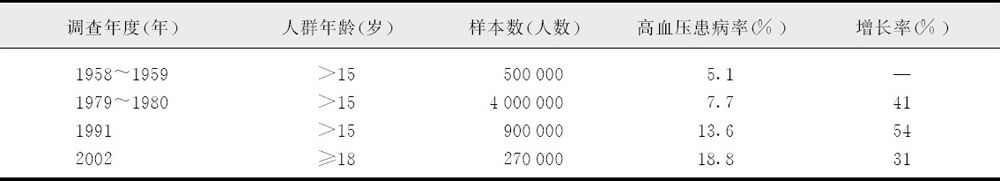
\includegraphics{./images/Image00017.jpg}
\end{table}

引自:《中国高血压防治指南》(2005年)修订版。

2005年5月在美国旧金山举行了第20届美国高血压学会(ASH)年会上,针对日益严重的高血压流行情况,会上宣布了高血压的新定义:高血压是一个渐进的,由复杂的和相互关联着的病因学引起的心血管症状。早期的症状常常在持续的血压升高前就有所表现。因此,高血压不能仅仅以离散的血压指标来分类。高血压的发展与功能性和结构性的心血管异常密切相关。这些异常损害心脏、肾脏、脑、血管系统和其他器官,从而导致过早的病态和死亡。制定新定义的宗旨就是要改进临床医生对高血压的理解、诊断和治疗的再认识。使他们对高血压的分类不再局限于血压值,而是必须考虑个体心血管的综合代谢症状,如肥胖、糖耐量异常、高胰岛素血症、低HDL、高LDL和高三酰甘油等因素,在高血压影响到靶器官以前,集中治疗各种导致发病和死亡的危险因素。因此,治疗高血压,不能仅仅以降低血压为终极目标,而是要通过综合性的治疗,包括营养、运动、心理等多种方案干预,改善病人的代谢情况,从而降低高血压发病率以及并发症的危害。

(一)高血压定义与分类

{1.诊断标准和新的定义}
 高血压是指人体循环收缩压和(或)舒张压持续升高。目前,我国采用国际上统一的标准,即收缩压≥140mmHg,舒张压≥90mmHg即诊断为高血压。

{2.分类}

(1)根据发病原因

1)原发性高血压:病因不明,在一定的遗传背景下由于多种后天环境因素作用使正常血压调节机制失去代偿所致;发病人数占总高血压病人数的90%~95%。

2)继发性高血压:某些疾病的一种临床表现,这些疾病包括急慢性肾炎、多囊肾、慢性肾盂肾炎、肾动脉狭窄、主动脉缩窄以及一些内分泌疾病(如甲状腺功能亢进、嗜铬细胞瘤、原发性醛固酮增多症、柯兴综合征等);发病人数占总高血压病人数的5%~10%。

(2)根据血压水平:表3-3是根据血压水平进行分类情况。

\begin{table}[htbp]
\centering
\caption{血压水平的定义和分类}
\label{tab3-3}
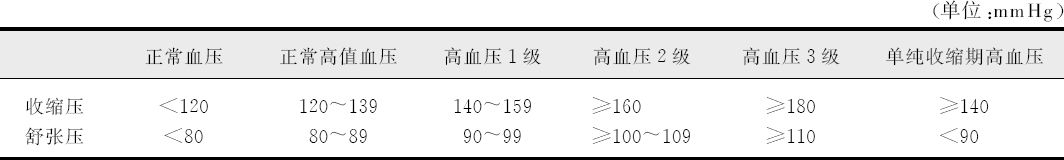
\includegraphics{./images/Image00018.jpg}
\end{table}

引自:《中国高血压防治指南》(2004年)。

(二)我国高血压患病人群现状

作为一种常见的心血管疾病,高血压已逐渐成为一个全球范围内的重大公共卫生问题。2002年中国居民营养与健康现况调查结果显示,我国高血压患病人群呈现如下三大特点。

{1.患病率、患病人数逐年上升}
 1991年患病率为14.6%,患病人数9000万;2004年患病率18.8%,患病人数1.6亿;同比增加3.1%,患病人数增加7000万。当今,我国每100个成年人中就有19人患有不同程度的高血压,而且,每年还以增加300万病例的速度递增。

{2.农村患病率上升迅速,城乡差距已不明显}
 大城市患病率为20.4%;中小城市18.8%;一类农村21.0%;二类农村19.0%;三类农村20.2%;四类农村12.6%。由此可见,随着生活方式的改变、生活水平的提高,高血压发病率在农村正呈明显向城市接近的趋势。

{3.人群高血压知晓率、治疗率、控制率仍然处于较低水平}
 1991年人群知晓率、治疗率、控制率分别为26.6%、12.2%、2.9%,而2004年相应的也仅为30.2%、24.7%、6.1%,这需要引起我们高度重视。由于健康的生活方式与合理的早期治疗可以使3/4的高血压病及其由此引发的慢性病得到有效控制,所以对高血压必须进行早期干预。

(三)营养因素对高血压发病的影响

{1.电解质}

(1)钠:健康成人每天钠盐的生理需要量为5g,多余的钠盐是导致高血压病的重要原因。我国的研究证明,膳食钠摄入量或钠钾比值无论在人群间或个体间都和血压呈显著正关联,人群间每人每天平均烹调用盐每相差3g,收缩压均值相差2.8mmHg。流行病学统计资料表明,每天吃15g食盐者,高血压发病率约为10%,如再增加食盐2g,则高血压发病率提高2倍。调查显示,每天人均食盐摄入量增加2g,收缩压和舒张压就能分别升高2.0mmHg及1.2mmHg。膳食中的高盐摄入是引起血压水平升高及高血压发病最重要的危险因素。研究结果显示,每天摄入食盐≥12g者患高血压的风险增高14%,每天食盐摄入量≥18g者则增高27%。我国北方人平均每天食盐量为15~20g,高血压患病率约达14%;南方人平均每天食盐量也达到12~13g,患病率为5%~7%。日本北海道农民,由于习惯于食用大量的腌制食品,日均食盐摄入量为26g,高血压病人竟高达40%。而食盐量极少的格陵兰岛的爱斯基摩人、中南美洲的印第安人、新几内亚和所罗门群岛的居民,几乎不存在高血压病人。由此可见,食盐摄入量与血压之间确有密切关系。

自20世纪以来,国内外学者就盐摄入量与血压的关系进行了广泛的人群流行病学研究,比较不同的国家之间,或同一国家的不同文化、不同地区人群之间盐摄入量与血压呈正相关,高盐摄入量与高血压发生有关。迄今报道的大多数人群研究证明,在极高盐摄入和极低盐摄入人群中,平均每天钠摄入量与高血压发生率呈正比,即低钠低血压、高钠高血压。在我国,北方地区摄盐量普遍高于南方,多项流行病学调查也显示,北方高血压的患病率高于南方。为了真实地反映盐与血压的关系,国际上于20世纪80年代中期进行了有名的Intersalt研究。这一研究包括全球范围32个国家的52个中心。该研究证实:①在52个中心之间,平均24小时尿钠排泄量与血压随年龄上升速度呈显著正相关;在各中心内,个体排钠量与血压显著正相关,至少在部分中心内此关系独立于体质指数和饮酒量;②在排钠量极低的4组人群中,其血压中位数和高血压患病率亦低。该研究有力地说明了钠盐与血压的关系。

(2)钙:钙是人体内含量最多的矿物元素。近10年来的临床研究表明,膳食钙能影响人的血压。一般认为,膳食中每天钙的摄入量<600mg可能会导致血压升高。这可能与钙有促进尿钠排出、调节激素潜在的血管活性作用以及调节交感系统活性有关。2002年中国居民营养与健康调查中发现,膳食钙与高血压呈弱的负相关。将钙的来源分为乳制品和非乳制品后,发现乳制品来源的钙与高血压呈显著负相关,而非乳制品来源的钙与高血压没有相关性。要说明的是,钙拮抗剂是治疗高血压的一种药物,由于它对细胞膜上的钙离子慢通道具有选择性阻滞作用,从而减少钙离子的内流,使得血管扩张、血压下降。补钙与使用钙拮抗剂之间不存在矛盾,同时应用可能有协同作用。

{2.脂肪和脂肪酸}
 脂肪酸引起血压升高和促进高血压血管病变与血浆游离脂肪酸组成有关,因为血浆游离脂肪酸对血管内皮细胞有直接作用:它们可进入细胞内作为第二信使;加入到细胞膜磷脂中改变膜的功能;生成有血管活性的二十烷类来影响细胞功能。高血压病病人血浆总饱和脂肪酸与正常对照组相比较是明显增高的,其中主要以豆蔻酸、棕榈酸及硬脂酸为主。研究还发现高血压病病人血浆反式油酸较正常对照组为高。

大规模前瞻性临床试验发现,空腹血游离脂肪酸(free fatty acid,
FFA)总体水平增高或血磷脂脂肪酸组成改变(亚油酸与多不饱和脂肪酸/饱和脂肪酸比值降低、软脂酸和花生四烯酸水平增高)与3年或6年内发生高血压的高危性独立相关。与正常血压者相比,原发性高血压病人血清FFA中,多不饱和脂肪酸(polyunsaturated
fatty acid, PUFA)水平降低(P=0.004),饱和脂肪酸(saturated fatty
acid, SFA)和单不饱和脂肪酸(monounsaturated fatty acid,
MUFA)水平有增高趋势(P=0.06和P=0.097),PUFA/SFA比值降低(P=0.000),PUFA/MUFA比值降低(P=0.000)。进一步研究发现原发性高血压病人存在空腹血FFA组成的改变,表现为PUFA水平降低和PUFA/SFA比值降低,前者主要是n-3PUFA水平降低为主,这种改变与舒张压水平升高相关,且独立于其他因素对血压的影响。空腹血个体脂肪酸水平改变提示存在α-亚麻酸代谢缺陷,且与肝脏的n-3去饱和酶活性降低有关。Grimsgaard等对4033名40~42岁健康男性研究发现,血浆磷脂中总脂肪酸和饱和脂肪酸(SFA)含量与血压水平呈正相关,而多不饱和脂肪酸的亚油酸含量与血压水平呈负相关。Zheng等通过对2488例中年人前瞻性临床研究发现,血浆胆固醇酯中亚油酸(C18:2)和PUFA/SFA比率的降低、软脂酸(C16:0)和花生四烯酸(C20:4,n-6)含量的升高,与高血压病的危险性相关。尤其腹内脂肪对血压的影响更大,其机制可能与下述因素有关:腹内脂肪细胞具有较高的代谢活性,其脂肪细胞可分解出大量游离脂肪酸(FFA),而从脂肪组织中分泌一些脂肪细胞因子参与代谢变化,导致脂质代谢紊乱,也使FFA升高,在异位组织沉积,降低血管平滑肌钠泵和钙泵活性,增强血管对缩血管物质的反应,导致血管收缩,FFA可使血管内皮功能受损,舒血管物质减少,提高交感神经的兴奋性,致使血压升高。同时升高的FFA也可损害压力感受器,促使血压升高。故腹内脂肪的增加,可使血压升高。

{3.蛋白质}
 1989年报告的中国10组人群对比研究,表明人群中平均动物蛋白质能量百分比与血压均值呈负相关。随后又在其中3组人群研究中证明个体膳食中动物蛋白质摄入量、24小时尿中牛磺酸排出量(反映膳食中含硫氨基酸摄入量),以及血、尿中与动物蛋白质有关的氨基酸均与血压呈显著负相关。提示在中国人群中动物蛋白质及有关的氨基酸如牛磺酸、赖氨酸等是血压的保护因素。2002年进行的中国居民营养与健康调查也得出类似的结论,并且显示出这主要是由动物蛋白引起的,植物蛋白与高血压呈正相关,提示我国居民膳食中动物蛋白的摄入不足。

{4.碳水化合物}
 对碳水化合物与高血压的关系在目前的研究比较少。在动物试验中有报道高脂肪、精制糖类(如葡萄糖、蔗糖)饮食会造成氧化负担过重,一氧化氮生物活性降低,从而引起高血压。但目前尚缺乏对人群相应的研究资料。

{5.其他因素}

(1)肥胖或超重:流行病学调查发现,体质指数(BMI)与血压水平呈正相关。研究发现,BMI是原发性高血压的一个独立危险因素。肥胖属于高血压的危险因素之一已属定论。文献报道,随着BMI的增加,血压进行性增高,肥胖与血压呈正相关。有研究的数据表明,发生高血压的危险性与体重的增加呈正比,肥胖组的高血压危险性是正常组的8倍以上,在20~30多岁时体重增加的人危险性最大。我国一项研究表明,在控制其他危险因素后,BMI每增加1个单位(kg/m\textsuperscript{2}
),5年内发生高血压的危险性增加9%。中美心血管病流行病合作研究显示,BMI每增加3kg/m\textsuperscript{2}
,4年内发生高血压的相对危险性增加50%以上。钱岳晟等研究采用24小时动态血压检测表明,体重增加10kg,24小时SBP增加3~5mmHg,DBP增加近2mmHg。对我国24万人群的汇总分析显示,BMI≥24kg/m\textsuperscript{2}
者的高血压患病率是BMI在<24kg/m\textsuperscript{2}
者的2.5倍,BMI≥28kg/m\textsuperscript{2}
者的高血压患病率是BMI在<24kg/m\textsuperscript{2}
者的3.3倍。男性腰围≥85cm,女性≥80cm,其高血压患病率是腰围正常者的2.3倍。

穆华等研究的结果显示:腹内脂肪与全天、白天、夜间舒张压和白天收缩压具有相关性,与全天、白天舒张压的相关性更好;在排除药物干扰因素后,腹内脂肪与全天、白天、夜间舒张压的相关性更显著(P<0.01)。研究也发现BMI与全天、白天、夜间舒张压具有正相关性,腰围与全天和白天收缩压有相关性,与夜间收缩压具有较好相关性。这说明BMI和WC对血压有影响,但均不能体现腹部脂肪具体分布对血压的影响,穆华等研究显示腹内脂肪对血压的贡献更大,腹内脂肪与24小时血压变化的相关性更全面,尤其是对夜间血压影响更明显。

体重影响血压,可能是由于:①血容量过多;②心排血量增加而周围血管阻力无相应下降;③交感神经系统活性增加;④肾上腺皮质功能亢进,水、钠潴留;⑤胰岛素抵抗。

(2)高胰岛素血症:胰岛素分泌增多会导致血压升高。胰岛素是一种非常有力的营养激素,血管内皮细胞、平滑肌细胞都有胰岛素的受体。过多的游离脂肪酸会引起高胰岛素血症、脂代谢紊乱。胰岛素使血管壁蛋白质合成增加、血管壁增厚、交感神经活性增强导致钠潴留,从而导致血压升高。

(3)胰岛素抵抗:胰岛素抵抗可能也是高血压病的发病因素之一。高血压病人胰岛素抵抗与其他各项代谢异常密切相关,合并胰岛素抵抗的高血压病人盐敏感性发生率、血脂及血尿酸水平均比无胰岛素抵抗的高血压病人高,这说明胰岛素抵抗可能是各项代谢异常的根源。

(4)饮酒:饮酒作为高血压的独立危险因素已经通过大量流行病学研究加以证实,尤其过量饮酒是发生高血压病的主要危险因素之一。酗酒是高血压、脑卒中的主要原因之一,特别是饮高度乙醇含量的白酒。俄罗斯人喜欢喝伏特加酒,脑卒中在世界上“名列前茅”,而欧洲人不饮白酒,多喝葡萄酒或啤酒,脑卒中人明显要少。中国高血压抽样调查结果表明,饮酒组高血压患病率比非饮酒组高39.9%,饮酒量与血压水平呈现剂量反应关系。饮酒量还与心血管疾病的危险度呈“U”形关系:适量饮酒,血中对冠心病有保护效应的高密度脂蛋白胆固醇含量增高;但长期过多饮酒,乙醇及其代谢产物乙醛可增加肝脏疾患与硬化、心肌损害和脑卒中、猝死的危险性。据推测,乙醇在低剂量的时候可能有扩张血管的作用,而在剂量较高时则对血管有收缩的作用。研究显示,男性每天乙醇摄入量>30g(相当于100g白酒),发生高血压的危险比每天乙醇摄入量<30g者增加3~4倍。每天平均酒精摄入量>60g(相当于约150g低度白酒)的人群,与每天酒精摄入量<20g(相当于约50g低度白酒)人群比,患高血压的危险性增加77%。据估计,这与每5人高血压病人中就有1人饮酒有关。经常饮酒者在饮酒期间,交感神经系统兴奋性增加、心率加快、血压随之升高、心脏负担加重。此外,长期大量饮酒还可以引起促肾上腺皮质激素水平升高,引起水、钠潴留,血容量增多,也能导致血压升高。不少脑溢血和心肌梗死是由于过量饮酒而诱发的。

(四)营养治疗原则

高血压的治疗是强调生活方式的调整,它既有助于高血压的预防又可以帮助高血压的治疗。生活方式的调整包括:减轻体重、增加运动、限制饮酒和减少钠盐的摄入以及采用合理的饮食模式。DASH(dietary
approaches to stop
hypertension)是一种富含蔬菜、水果、低脂乳制品、果仁、白肉,减少红肉、饱和脂肪酸和含糖饮料的摄入饮食模式。该食谱的特征从营养角度上含低脂肪、低胆固醇、高钙、高钾、高镁及高纤维。美国NIH的国立肺血液研究所主持的两个多中心实验表明:DASH饮食可以明显降低血压。2001年Sack
FM等在DASH研究的基础上进一步研究了DASH和钠的关系,认为DASH联合低钠能更有效的降低血压。从对DASH饮食模式的研究可以给我们这样一个观点,即控制高血压不是单纯的增加或减少某个营养元素,而是通过改变饮食模式,通过食物中营养因素的互相影响,协同作用,从而发挥最大的降压效果。

{1.限制钠盐摄入}
 WHO在预防高血压措施中建议每人每天摄盐量应控制在6g以下。我国膳食中的钠80%来自于烹饪时的调味品以及含盐量高的盐制品。因此,少盐首先要提倡淡味饮食,即食物菜肴中有轻度咸味即可,用盐量约为正常饮食的1/3左右,减少调味品的使用量。可使用低钠食盐和无盐酱油;尽量不食咸肉、腊肉、咸菜等含盐量较高的腌制品;多选用低钠食物,如面粉、大豆、豆腐、毛豆、马铃薯,以及新鲜蔬菜。

{2.调节饮食模式}

(1)高钾、高钙、高镁的摄入,增加膳食纤维:增加富含钾、钙、镁的食物。在膳食中摄入钙的时候应注意某些草酸含量较高的蔬菜如菠菜、苋菜、茭白、竹笋、荸荠等,不宜与含钙高的食物一起食用。因为这些食物中含有丰富的草酸成分,容易与钙形成不溶性的草酸钙,从而不利于人体对钙的吸收。

(2)限制脂肪总摄入量,减少饱和脂肪酸,增加多不饱和脂肪酸的摄入:脂肪过量摄入是引起高血压的重要危险因素。因此,高血压病人必须限制脂肪的总摄入量,使其不超过每天总能量的25%。膳食中饱和脂肪酸、单不饱和脂肪酸和多不饱和脂肪酸之比维持在0.8∶1.2∶1。

(3)摄入足够的优质蛋白质:除并发肾功能不全者外,高血压病人不应过分限制蛋白质的摄入,尤其应增加一些优质蛋白质的摄入。例如,鱼类蛋白质中的含硫氨基酸能增加尿钠排泄,从而减轻钠盐对血压的不利影响,起到降压和减少脑卒中的作用。大豆蛋白质具有保护心脑血管的作用,虽然对血压无明显影响,但可降低高血压病人的脑卒中发生率。

{3.控制体重,增加运动}
 肥胖或超重会导致血压升高,增加高血压的发病率。因此,减肥不仅是对肥胖本身的治疗,而且对控制高血压也是十分必要的。

{4.限制饮酒}
 大量饮酒是高血压的危险因素之一,饮酒后体内的肾上腺皮质激素及儿茶酚胺等内分泌激素升高,通过肾素-血管紧张素系统等使血压升高,因此高血压病人每天饮酒量限制在25g酒精以下,女子应更少,青少年不宜饮酒。

\hypertarget{text00004.htmlux5cux23mllj9}{%
\subsection{营养与脂代谢紊乱}\label{text00004.htmlux5cux23mllj9}}

2002年《中国居民营养与健康状况调查》结果显示,我国≥18岁成人血脂异常患病率为18.6%,18~44岁、45~59岁和≥60岁人群的患病率分别为17.0%、22.9%和23.4%;男性为22.2%,女性为15.9%;城市为21.0%,农村为17.7%。>18岁成人高胆固醇血症患病率为2.9%,胆固醇边缘性升高率为3.9%;高三酰甘油血症患病率为11.9%;低高密度脂蛋白血症患病率为7.4%。由此可见,我国目前≥18岁的血脂异常病人估计达1.8亿之多。其中,以高TG、低HDL为主。中、老年人血脂异常患病率接近,发病年龄趋向年轻化,城乡差别并不大。脂质代谢紊乱是导致心脑血管疾病的主要原因之一,常与体重超重、肥胖、高血压病、2型糖尿病和痛风等伴随。它与饮食过度和运动量减少高度相关。脂质代谢紊乱病人首选的治疗方法是合理饮食和适宜运动。因此,是一类与营养治疗密切相关的疾病。

(一)概述

血脂及脂蛋白代谢异常(简称为血脂异常)是指体内某些脂质或脂蛋白成分过高或过低的表现。临床常见的血脂异常有以下3种:血清总胆固醇(TC)或低密度脂蛋白(low
density lipoprotein,
LDL)水平过高;血清三酰甘油(TG)水平过高;血清高密度脂蛋白(high
density lipoprotein, HDL)水平过低。

(二)血脂代谢紊乱分类及诊断

{1.根据异常脂蛋白的表型,辅以其他方法对血脂异常进行分类}

(1)原发性:罕见,属遗传性脂代谢紊乱疾病。

(2)继发性:常见于控制不良糖尿病、饮酒、肥胖病、甲状腺功能减退症、肾病综合征、肾透析、肾移植、胆道阻塞、口服避孕药等。

{2.根据脂蛋白组分含量的不同进行分类}
 如高胆固醇型、高三酰甘油型和混合型高脂血症等。

{3.脂代谢紊乱诊断标准}  中国血脂异常诊断标准见表3-4。

\begin{table}[htbp]
\centering
\caption{中国血脂异常诊断标准(1997年)}
\label{tab3-4}
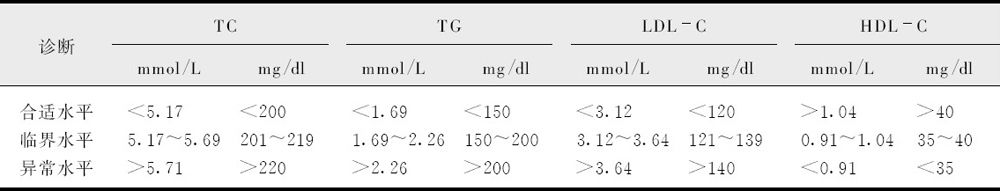
\includegraphics{./images/Image00019.jpg}
\end{table}

(三)营养因素对高脂血症的影响

{1.胆固醇}
 一般认为,膳食中胆固醇的摄入是引起血浆胆固醇升高的最主要因素,因此胆固醇摄入不宜过高,应该严格控制。有研究显示,正常成年人,膳食胆固醇摄入量以不超过300mg/d为宜,每增加100mg,男性血浆胆固醇水平将增加0.038mmol/L,女性增加0.073mmol/L。虽然随胆固醇摄入量增加,其吸收率下降,但其绝对量仍然会增加。近年来也有不同的研究结果,认为年龄是影响TC的主要因素,而蛋类和肉类等食物的摄入量对血清胆固醇的影响有限。甚至蛋类与TG呈负相关。由于缺乏大样本的调查研究,目前的证据尚不能就此作出结论。我们仍然可以这样认为,在严格控制胆固醇摄入的饮食模式中,不应完全戒断蛋类的摄入。

{2.饱和脂肪酸(saturated fatty acid, SFA)}
 膳食中饱和脂肪酸含量过高,也可使血浆胆固醇升高。主要原因是饱和脂肪酸能够抑制低密度脂蛋白受体活性。其作用机制可能与以下5个方面有关:①抑制TG在肝内合成;②促进调节性氧化类固醇形成;③降低细胞表面LDL活性;④促进无活性非酯化胆固醇转入活性池;⑤降低LDL与其受体的亲和性。

不同长度的碳链的SFA对血脂的作用不同。碳原子<12、≥18的SFA对于血清TC没有影响。但是,含12~16个碳原子的SFA如月桂酸(C12:0)、肉豆蔻酸(C12:0)、棕榈酸(C16:0)可明显升高血清TC、LDL水平。其中,月桂酸、肉豆蔻酸在牛乳脂、椰子油中含量最多;棕榈酸主要存在牛乳脂、牛油、猪油、羊油中。

{3.多不饱和脂肪酸(polyunsaturated fatty acid, PUFA)}
 多不饱和脂肪酸对人体内脂质代谢的影响作用包括以下几个方面。

(1)促进胆固醇代谢,减少脂质在肝脏和动脉壁沉积:当膳食中多不饱和脂肪酸充裕时,胆固醇便与之结合形成胆固醇酯,促其形成胆酸而从肠道排出。有研究表明,血胆固醇与膳食中SFA的摄取量呈正比,与膳食中不饱和脂肪酸的摄取量呈反比。

(2)提高血清中HDL含量,对降低血脂有一定作用:膳食中所摄入的饱和脂肪酸被吸收后,在肝脏中形成TG,进而转变为LDL,SFA可抑制低密度脂蛋白受体的活性,因而减少血中胆固醇的消除,由于胆固醇的吸收增加,血脂合成增多,消除减少,故使血脂升高。而多不饱和脂肪酸消化吸收后,在肝脏中不形成TG和LDL,而是与肝脏细胞分泌的载脂蛋白结合成为HDL,HDL作为胆固醇的受体与胆固醇进行结合形成HDL-C,而后通过血液循环送入肝细胞中,胆固醇形成胆汁酸排出体外而被消除,降低血脂。

(3)降低血小板的凝集能力,减少血栓的产生:血管收缩和血小板聚集是造成动脉粥样硬化和促进血液凝固并引起栓塞现象的另一个重要因素。而多不饱和脂肪酸(主要是EPA)可使磷蛋白酯酶活性增高,抑制血小板凝集,并且还能增加组织纤溶活化剂的溶栓作用,降低纤维蛋白原水平及血液黏稠度,增加血液的流动性,从而防止血栓的形成。

(4)减少血管炎性反应:血管在发生炎性反应后会促使脂质在动脉壁上的沉着而引起动脉粥样硬化的发生,而多不饱和脂肪酸能在血管的损伤面加强白细胞的作用,从而降低炎症反应,延缓血管损伤部位血管硬化的进程。

(5)提高免疫力:多不饱和脂肪酸能够促进人体防御系统功能,使血液中的脂肪酸谱向着对人体健康有利的方向发展,从而有利于防止其他可以引发和加重心脑血管疾病的发生。

{4.单不饱和脂肪酸(monounsaturated fatty acid, MUFA)}
 单不饱和脂肪酸指碳链中含有1个双键的不饱和脂肪酸。油酸、橄榄油、花生油、茶油中富含单不饱和脂肪酸。已有研究表明,单不饱和脂肪酸具有降低血清LDL和胆固醇的作用,并且有助于提高血清的HDL的作用。

{5.反式脂肪酸(trans fatty acid, TFA)}
 膳食中的反式脂肪酸,多产生于氢化油脂,例如人造黄油。已有研究表明,反式脂肪酸具有增加胆固醇、升高LDL-C、降低HDL-C等作用,明显增加患心血管疾病的危险性。

{6.碳水化合物}
 大量进食碳水化合物,尤其是缺乏纤维素的双糖和单糖类会使得糖代谢增强,细胞内的ATP增加,从而脂肪合成增加,血清VLDL-C、TC、TG、LDL-C增高,HDL-C降低。

{7.膳食纤维}
 植物性食物中的谷固醇和膳食纤维可以影响机体对胆固醇的吸收,从而降低胆固醇水平。可溶性膳食纤维比不溶性膳食纤维的作用更强,前者更多存在于大麦、燕麦、豆类以及水果等。

{8.维生素}

(1)维生素C:有研究表明,维生素C对血脂水平具有一定的降低作用,这种作用可能通过以下两种途径实现:①促进胆固醇降解、转为胆汁酸,从而降低血清总胆固醇TC水平;②增加脂蛋白脂酶的活性,加速血清VLDL-C及TG降解,从而降低血清TG水平。除了降低血脂的作用,维生素C又是一种重要的生理性抗氧化剂,在对抗由自由基引发的脂质过氧化反应中发挥着重要作用。

(2)维生素E(也称生育酚):近年来大量研究证明,给予维生素E可延缓动物动脉粥样硬化病变的形成。具体的机制目前尚不明确,推测维生素E可能通过减少氧化修饰的LDL(OX-LDL)的产生,或通过减少泡沫细胞的形成,保护血管。此外,维生素E可能影响参与胆固醇分解代谢的酶的活性,加快胆固醇的转运与排泄,从而对血脂水平起调节作用。

但须指出的是,尽管维生素E有保护心血管的作用。但目前无证据表明,补充维生素E可以降低心血管疾病的发病率。它无法抵消因抽烟、高脂饮食及其他不良的生活习惯所带来的负面影响。因此,不能作为调节血脂紊乱的主要方法。

{9.微量元素}  有研究表明,许多微量元素与脂代谢紊乱有关。

(1)锌:锌在人体中含量为2~3g,以辅酶形式存在,对机体代谢起着广泛的调节作用。缺锌可引起血脂代谢异常已被大量实验研究所证实。研究表明,膳食中锌含量对血脂代谢有重要影响。但是,摄入量要适当。中国营养学会推荐的每天锌摄入量成人为15~20mg。

(2)铜:铜对血脂代谢有一定影响,铜含量低下会引起血清LDL-C异常升高。铜在生物代谢的某些酶中起催化作用。人类血浆中正常的铜含量约为1000μg/L,成人每天摄入量应为2.0mg。

(3)铬:铬常以有机复合物形式存在,称为葡萄糖耐量因子,是葡萄糖和脂质代谢的必需微量元素,易被吸收,成人每天需要量为0.05~0.2mg。铬存在于麦胚、麦皮、未精制多糖和酵母中。

(4)锰:锰是参与葡萄糖和脂肪代谢的多种酶的激活剂(如丙酮酸羧化酶、超氧化物歧化酶、葡萄糖酰基转移酶等),锰化铁也是合成鲨烯和胆固醇的羟甲戊酸激酶的辅因子。成人体内锰的含量为10~20mg,推荐成人每天适宜摄入量为3.5mg。

{10.其他}
 近年来,有很多新的研究方向,对食物中和植物中存在的一些特殊的营养物质,例如大豆中富含的大豆皂苷(soyasaponins)和茶叶中富含的茶多酚、葡萄籽和皮中含有的葡多酚等,均有调节血脂及抗脂质过氧化的作用,从而达到预防脂代谢紊乱的作用。

(四)饮食治疗

饮食治疗是治疗脂代谢紊乱的重要手段,即使在进行药物降脂治疗时,也要同时进行膳食控制,以提高疗效。若肥胖伴脂质代谢紊乱,则参见肥胖病治疗原则。

{1.控制总能量、保持能量摄入与消耗的平衡}
 根据年龄、性别、工作性质给予合理能量。三大营养素的比例为碳水化合物50%~60%、蛋白质10%~20%、脂肪<30%;保持能量均衡分配,三餐比3∶4∶3;适当增加运动,保持理想体重。

{2.碳水化合物}
 主食以谷类为主,粗细搭配,粗粮中可适量增加玉米、莜面、燕麦等成分,保持碳水化合物供能量占总能量的55%左右。限制精制糖和含糖类的甜食,例如点心、糖果和饮料等。

{3.蛋白质}
 增加豆类食品,提高蛋白质利用率,以干豆计算,平均每天应摄入30g以上,或豆腐干45g或豆腐75~150g。大豆蛋白质的氨基酸种类比较齐全,因而营养价值相对较高。并且,大豆中几乎不含胆固醇,相反含有豆固醇和大豆皂苷,可以起到抑制机体吸收胆固醇的作用。大豆中所含的亚油酸、磷脂、纤维素等都对心血管系统有保护作用。牛奶中不仅蛋白质含量高,而且含有羧基与甲基戊二酸,能够抑制人体内的胆固醇合成酶的活性,从而降低血中胆固醇的含量。牛奶中富含的钙质和乳清酸都能减少人体对胆固醇的吸收。故而,高血脂病人可以选择补充适量的低脂奶、脱脂奶或酸奶。

{4.脂肪}
 每天总脂肪供能量不超过总能量的30%。在动物性食物的结构中,增加含脂肪较低而蛋白质较高的动物性食物,如鱼、禽、瘦肉等,并减少陆生动物脂肪;限量使用植物油,少用动物脂肪。每人每天用量以25~30g为宜;增加n-3多不饱和脂肪酸EPA、DHA摄入量。多吃水产品,尤其是含鱼油较高的海产品,争取每周食用2次或以上;轻度胆固醇升高者,膳食中胆固醇摄入量每天不宜超过300mg/d。血浆胆固醇中度和重度升高者,膳食中胆固醇摄入量应<200mg/d。

{5.维生素、无机盐、植物纤维及微量元素}

(1)保证每人每天摄入的新鲜水果及蔬菜达500g以上,注意增加深色或绿色蔬菜比例。膳食成分中应含有足够的维生素、无机盐、植物纤维及微量元素。例如苹果中含有类黄酮,可以抑制OX-LDL的形成,从而发挥抗动脉粥样硬化的作用。

(2)适当减少食盐摄入量。

(3)多摄入含硫化物丰富的大蒜和洋葱,以及多糖类物质,如香菇、木耳。

(4)限制饮酒:每天摄入乙醇以20g为限,或者白酒不超过50g。葡萄酒对冠心病有保护作用,可适量饮用。

(5)多饮茶:茶叶中含有茶多酚等物质,具有抗氧化作用和调节血脂、防止动脉粥样硬化的作用,尤其是绿茶,作用优于红茶。少饮咖啡,如果大量饮用咖啡,尤其是不过滤的冲煮方法,有可能使血中游离脂肪酸增加,血清胆固醇升高。

\hypertarget{text00004.htmlux5cux23mllj10}{%
\subsection{心血管疾病的控制原则}\label{text00004.htmlux5cux23mllj10}}

合理膳食,适量运动,加上控制吸烟,有助于控制心血管疾病的发生、发展。在许多工业化国家已证明取得很大成功。芬兰在20世纪60年代冠心病死亡是世界之最,从70年代起开展了全国性的以改变不健康膳食为主要内容的干预计划(最著名的为北加里省的防治计划),通过20年的努力使冠心病死亡及危险因素水平明显下降。美国冠心病死亡率从20世纪30年代开始持续上升,到了60年代上升到顶点。此时,美国在全国范围内开展了健康生活方式的教育,其中健康膳食是很重要的健康教育内容,随之冠心病死亡率开始以每年2%的速度下降。

(一)膳食指导建议

心血管疾病的发生、发展是一个长期积累的结果,它和整个生命过程中的膳食、营养及生活方式都有关。近年来,国际营养学界对膳食指南认识方面的一个方向性转变,是从以营养学为基础的膳食指南转向以食物为基础的膳食指南。这是因为,如果只重视营养素摄入的调查,而不注重改变膳食模式,是不可能达到目的的。因此,根据我国人民的膳食习惯及《中国居民膳食指南》,对预防心血管疾病提出如下建议。

(1)每天摄入多种谷类、豆类、根茎类食物,摄入量以占总能量的55%~65%为宜,并尽量多选用粗加工的谷类。

(2)控制红肉的摄入量,应限制在80~100g以内,多选用鱼、禽、蛋代替红肉,每周至少1次鱼肉、1次鸡肉、1~2次豆制品、1~2次海产品。

(3)限制脂肪含量高,特别是动物性脂肪含量高的食物,选择植物油,特别是不饱和脂肪酸含量高、氧化程度低的油脂,少用肥肉和荤油及含胆固醇高的动物内脏、鱼子等。

(4)多吃蔬菜、水果和薯类,每天蔬菜、水果量应为400~600g。

(5)避免体重过重或过轻,整个成人期的体重增加应限制在5kg以内。

(6)坚持适当运动,活动量与食量要平衡,尤其工作缺乏体力活动者,应每天进行一定量的运动。

(7)建议戒烟、酒,假如饮酒应有节制,以每天白酒1~2两为限(以20g/d乙醇为限)。

(8)少吃盐腌、熏制及纯糖食物,食盐摄入量为6g,有高血压家族史者应在5g以内。

(9)多饮奶类,多吃鱼类,有条件者可每天饮奶250~500ml。

(10)要有健康的生活方式,保持健康的心态。

心血管疾病膳食指导原则应供给低钠、高钾、高钙饮食,膳食搭配应多补充含钙、钾丰富的食物,如奶类、豆制品、蔬菜及水果等。

(二)美国心脏病协会对饮食与生活方式的建议

美国心脏病协会营养委员会在《AHA
2000饮食指导》的基础上,并结合近年来的临床及试验观察结果组织制定了《AHA
2006饮食及生活方式建议》,发表在《循环》杂志上(Circulation,2006,114:82~96)。《建议》包括:平衡能量摄入和体力活动,保持正常体重;多吃蔬菜和水果;选择全谷物、高纤维的食物;一周至少吃2次鱼;限制饱和脂肪酸(主要为动物脂肪)的摄入少于总能量的7%,反式脂肪酸(主要来源于用于煎炸和烘烤的商业用氢化油)的摄入少于总能量的1%;通过选择瘦肉、蔬菜、脱脂或低脂(含脂量为1%)奶制品等保证每天摄入<300mg胆固醇;尽量少食用添加糖的饮料及食物;少摄取食盐,建议每天食盐量<2.3g;适量饮酒或不饮酒;在外就餐时也要遵守此饮食及生活方式建议。AHA期望按照《建议》能使人们保持健康全面的饮食,多参加体育锻炼,不吸烟,BMI控制在18.5~24.9kg/m\textsuperscript{2}
,低密度脂蛋白胆固醇<2.6mmol/L,血压<120/80mmHg,空腹血糖≤5.55mmol/L,这样做就可大大减少心血管疾病的危险。推荐食用水果、蔬菜、全麦等植物来源的抗氧化剂。而其他抗氧化添加剂、大豆蛋白、叶酸及其他B族维生素、植物化学物质(如类黄酮)等对于心血管是否有益目前尚无定论。但AHA建议冠心病病人每天服用约1g二十碳五烯酸(EPA)和二十二碳六烯酸(DHA),高三酰甘油病人每天服用EPA和DHA共2~4g。每天服用植物固醇作为降脂治疗。

(三)WHO对心血管疾病病人的膳食建议

{1.脂肪}
 每天的总脂肪摄入量应保持在15%~30%,SFA的摄入量应低于每天能量摄入量的10%,高危人群应低于7%。PUFAs的摄入量应为能量摄入量的6%~10%,并应保证n-6PUFAs和n-3PUFAs摄入量的平衡,两者分别应为能量摄入量的5%~8%和1%~2%。单不饱和脂肪酸(10%~15%总能量)。反式脂肪酸的摄入量应低于每天能量摄入量的1%。

{2.水果和蔬菜}
 每天摄入≥400g蔬菜或水果(包括浆果、绿色阔叶和十字花科蔬菜)以及全麦和豆类,可以从这些植物性食物中获得钾的摄入量,每天膳食中钾摄入量为70~80mmol,可降低血压,预防脑卒中和心律失常。植物性食物还含有丰富的膳食纤维(NSP),膳食纤维可以预防冠心病,还可以降低血压。通过食用水果、蔬菜和全麦谷类可以达到适宜的摄入量。

{3.鱼类}
 建议多吃鱼(每周1~2份),有助于预防冠心病和缺血性脑卒中。每份鱼应能提供200~500mg的EPA和DHA。素食者应保证摄入适量的植物来源的α-亚麻酸。

{4.减少钠的摄入量}
 每天盐(氯化钠)摄入量应减少1/3,尽可能<5g/d或<90mmol/d。目前认为每天的钠摄入量不超过70mmol或1.7g,对血压降低有益。

{5.限制饮酒}
 每天饮酒超过3个单位(每单位约等于含10%酒精的酒100ml或含40%酒精的酒25ml)者,应减少酒精摄入量。

{6.控制体重}
 鼓励超重或肥胖者减重,包括降低饮食能量摄入和增加运动。建议每周的大多数时间每天至少进行30分钟,且是中等强度的体力活动(如快走)。运动量更大、强度更高的体力活动的有益作用更强。

\hypertarget{text00004.htmlux5cux23mllj11}{%
\section{ 营养与肥胖}\label{text00004.htmlux5cux23mllj11}}

肥胖病是由于遗传、环境等特定的生物化学因子引起的一系列进食调控和能量代谢紊乱,使体内能量摄入大于消耗,能量代谢失衡,体内脂肪积聚过多、体重增加所致的一种常见的营养与代谢性疾病。

肥胖病的危害不仅是肥胖病本身会影响美观及使日常生活不便而引起的身心障碍和可能带来的社会歧视问题,更严重的是肥胖病是许多疾病如2型糖尿病、冠心病、高血压、脂质代谢异常、痛风(或高尿酸血症)、睡眠呼吸暂停综合征、胆囊炎、胆石症、关节炎及某些癌症发病的基础。大约80%的肥胖成人有1种、40%有2种以上上述的病态(症状)的聚集现象。肥胖病的发病率在过去10年中几乎增加1倍。肥胖病所带来的直接或间接的耗费约占国家卫生经费的10%。

肥胖病在富裕国家中由于食品供应丰富、静坐生活方式增多而普遍多见,但在社会福利和卫生保健工作较好的国家,单纯性肥胖病的检出率反而控制在较低水平,如瑞典仅为2%。近年来发展中国家肥胖检出率呈现快速增长,表明单纯性肥胖病应是发达国家和发展中国家共同面临的问题。据我国2004年10月卫生部、科技部、国家统计局发布的《中国居民营养与健康现状》显示,我国18岁及以上成年人中超重率为22.8%、肥胖率为7.1%,也就是说,我国≥18岁的成年人大约有2.6亿超重和肥胖者。大城市成年人有一半的人超重和肥胖(男性为45.9%,女性为39.8%),农村成年人也有1/4~1/3超重和肥胖。与1992年比较,我国超重率上升了38.6%、肥胖率上升了80.6%。2002年大城市7~17岁儿童超重率达13.1%,肥胖率为8.1%,已向发达国家水平发展。

尽管与美国等西方国家相比,我国的肥胖患病率相对较低,但是肥胖病的快速增长,尤其在儿童中令人惊讶。全国儿童体质调研资料表明,1985~2000年间,7~18岁儿童的体重超重率增长了28倍,肥胖率增长了4倍,这一增长趋势在男童中尤为明显。

\hypertarget{text00004.htmlux5cux23mllj12}{%
\subsection{评价指标与诊断}\label{text00004.htmlux5cux23mllj12}}

(一)定义

肥胖病是机体能量摄入超过能量消耗导致体内脂肪积聚过多及分布异常所致的一种常见的代谢性疾病。

肥胖者不仅体内脂肪细胞数量增多和脂肪细胞体积增大,且体内脂肪分布明显异常,主要集中在腹腔和内脏器官。

(二)临床评价肥胖病的指标

{1.体质指数(body mass index, BMI)}
 BMI=体重(kg)/身高(m)\textsuperscript{2} 。

{2.腰围(waist circuit, WC)}
 WC可确定腹部脂肪分布引起肥胖病相关疾病危险度,是腹内脂肪量和总体脂的一个近似指标。我国中心性肥胖的标准:男性腰围≥85cm,女性腰围≥80cm。

中国成人超重和肥胖的体重指数、腰围界限值与相关疾病危险关系见表3-5。

\begin{table}[htbp]
\centering
\caption{中国成人超重和肥胖的体重指数和腰围界限值与相关疾病危险关系\textsuperscript{*}}
\label{tab3-5}
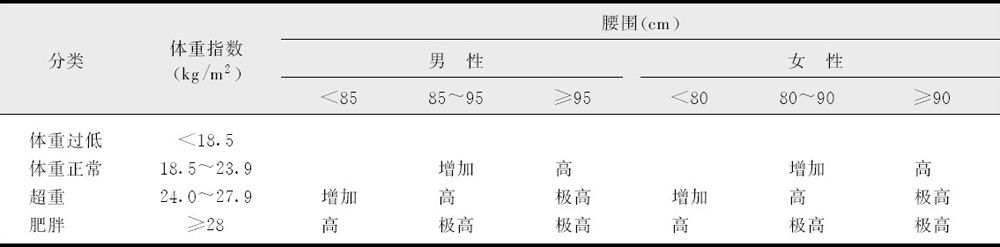
\includegraphics{./images/Image00020.jpg}
\end{table}

注:*相关疾病指高血压、糖尿病、血脂异常和危险因素聚集。

{3.腰臀比(waist to hip nation, WHR)}
 WHR是腰和臀围的比值。一般认为WHR>0.9(男性),或>0.8(女性)为中心性肥胖,但其值随着年龄、性别及人种不同而不同。

{4.标准体重(standard body weight)}

标准体重(kg)=身高(cm)-100(适用于身高<155cm者)

标准体重(kg)=身高(cm)-105(更适合亚洲国家)

标准体重(kg)=[身高(cm)-100]×0.9(适用于身高>155cm者)

{5.其他指标}
 双能量吸收测量法(包括双能量X线吸收测量法和双光子吸收测量法)及电阻抗测量法等均可以较精确地推算出体脂量,但这些方法更适用于科研。CT和MRI是评估内脏脂肪组织较准确的方法,但均为非常规方法。

(三)肥胖的诊断

{1.按标准体重诊断}
 超重:体重高于标准体重20%;轻度肥胖:体重高于标准体重20%~30%;中度肥胖:体重高于标准体重30%~50%;重度肥胖:体重高于标准体重50%。

{2.按BMI诊断}
 2000年WHO制定的BMI界限值为25.0~29.9kg/m\textsuperscript{2}
为超重,≥30kg/m\textsuperscript{2} 为肥胖。

{3.按WC诊断}  WHO建议,男性>94cm,女性>80cm可作为肥胖。

{4.按WHR诊断}  男性WHR>0.9,女性>0.8可作为中心性肥胖。

{5.按脂肪含量诊断}
 按体内脂肪所占的百分比计算,男性>25%,女性>30%,可诊断为肥胖病。

{6.儿童、青少年肥胖的诊断}  见表3-6、3-7。

\begin{table}[htbp]
\centering
\caption{中国男生以BMI为指标的超重、肥胖筛查的3个暂定标准与NCHS的标准比较}
\label{tab3-6}
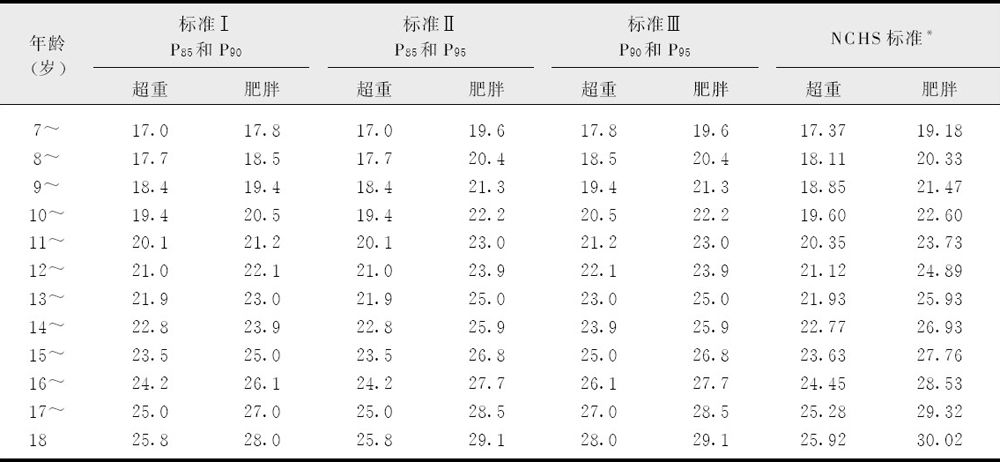
\includegraphics{./images/Image00021.jpg}
\end{table}

注:*美国国家健康统计中心(NCHS)标准。

\begin{table}[htbp]
\centering
\caption{中国女生以BMI为指标的超重、肥胖筛查的3个暂定标准与NCHS的标准比较}
\label{tab3-7}
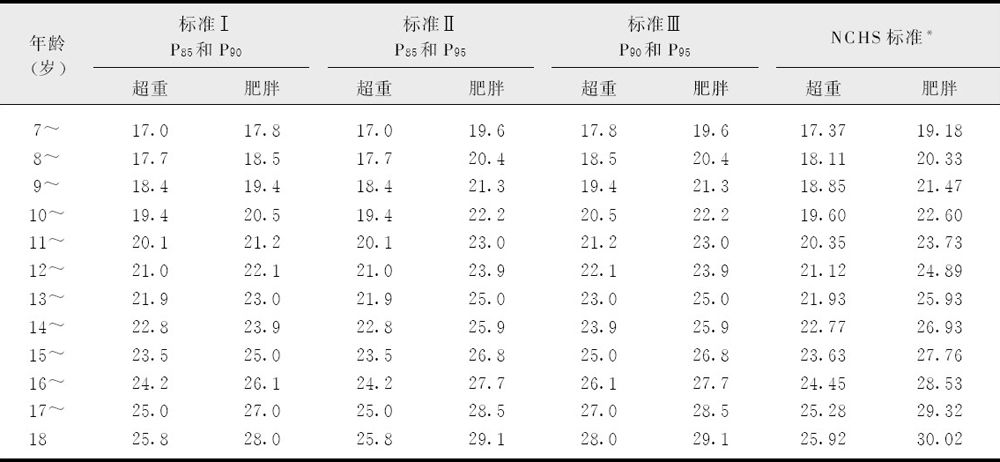
\includegraphics{./images/Image00022.jpg}
\end{table}

注:*美国国家健康统计中心(NCHS)标准。

\hypertarget{text00004.htmlux5cux23mllj13}{%
\subsection{肥胖病的分类和影响因素}\label{text00004.htmlux5cux23mllj13}}

(一)肥胖病的分类

{1.单纯性肥胖病}
 病人一般体态匀称、皮下脂肪分布均匀。其病因主要是遗传因素与环境因素所引起的不良的正能量代谢,最终导致脂肪细胞体积增大或同时脂肪细胞数量增多且分布异常,体重增长。

{2.继发性肥胖病}
 继发于某种疾病所引起的肥胖,一般均有原发性疾病存在。主要包括:①下丘脑病变:炎症、创伤、出血及肿瘤等引起肥胖病变;②垂体病变:垂体瘤、垂体前叶功能减退症;③甲状腺功能减退症;④皮质醇增多症:肥胖呈向心性分布,同时伴有满月脸、高血压、多血质外貌、痤疮及皮肤紫纹等。如要确诊皮质醇增多症,应做实验室检查确定;⑤多囊卵巢综合征:有多毛及男性化。

(二)肥胖病的影响因素

{1.遗传因素}
 遗传学研究表明,人类体重的变异,70%为遗传因素所致。双亲中一方为肥胖,其子女肥胖率为50%;双亲均为肥胖,子女肥胖率为80%。另有研究者调查的一组肥胖儿童中,其39%为母亲有肥胖、12%为父亲有肥胖、18%为双亲有肥胖。肥胖常伴有多种基因的改变所致基因多态性,故肥胖为多基因遗传。遗传因素对于肥胖的形成具有一定作用,但不是唯一决定性的,还有其他因素,如包括环境因素及年龄因素等。

{2.环境因素}
 遗传因素(基因的多态性)仅增加人体对肥胖的易感性,促进肥胖的环境因素对多种易感基因表达的影响也是一个重要的因素。

社会的进步、人们生活水平和机械化劳动程度的明显提高,以及教育程度相对偏低的中下层人群中常导致总能量摄入明显增多及三大产能营养素(碳水化合物、脂肪、蛋白质)结构配比明显不合理,静态行为随着机械化程度的提高而明显增加,导致能量消耗减少。

不良的饮食生活习惯和行为偏离、民族习俗等,如快餐类饮食,喜食高糖类、高脂类、油炸类等高能量食物;饮用大量具有能量的饮料及酒类;看电视进食;临睡前进食;进食速度快等,均可致能量摄入大于能量消耗。

{3.年龄因素}
 随着年龄增长,垂体前叶功能逐渐减退、内分泌代谢功能下降,导致人体由合成代谢为主逐渐转为以分解代谢为主,以致代谢失去平衡,细胞功能下降,人体体成分改变,体脂群逐渐增加、分布异常,瘦体组织群逐渐减少,总体水分减少。临床表现为对糖、脂肪代谢能力明显下降。中老年人群在摄入等同能量时与年轻人群相比更易肥胖。

(三)膳食、生活方式因素

{1.进食过量}
 超重/肥胖症是能量的摄入超过能量消耗以致体内脂肪过多蓄积的结果。工业发达国家的肥胖症患病率远远高于不发达国家,其原因之一是发达国家人群的能量和脂肪摄入(尤其是饱和脂肪的摄入量)大大高于不发达国家。随着我国的经济发展和食物供应丰富,人们对食物能量的基本需求满足以后,膳食模式发生了很大变化,高蛋白质、高脂肪食物的消费量大增,能量的总摄入往往超过能量消耗。与我国传统的膳食模式相比,很多城市,尤其在大城市的人们摄入富含高能量的动物性脂肪和蛋白质增多,而谷类食物减少,富含膳食纤维和微量营养素的新鲜蔬菜和水果的摄入量也偏低。已有研究证明含脂肪多而其他营养素密度低的膳食,引起肥胖的可能性最大。研究还发现含糖饮料与儿童肥胖的发生率有关。有一项研究显示,每天每增加摄入一份含糖饮料,发生肥胖的优势比增加1.6倍,这与增加能量的摄入有关。另有研究表明,从含糖软饮料摄入过多的能量与成人肥胖患病率增加有关。研究指出含糖软饮料消费增加的妇女,每天的总能量摄入亦增加,平均每天增加1498kJ(358kcal),而且增加的能量摄入绝大多数来自软饮料,并且发现对果汁酒、果汁以及含糖软饮料亦是这种情况。这项结果亦支持了下述发现,即:个体增加液态碳水化合物的摄入,并不会相应减少固体状食物的摄入,而是相反,导致更多的能量摄入。一罐12盎司(约340g)的含糖苏打水的能量为627kJ(150kcal),平均含糖40~50g。如果在典型的美国饮食中增加了这些能量,而不相应减少其他的能量供应时,每天饮用一罐苏打水将导致1年后体重增加6.75kg(15磅)。液态碳水化合物携带的能量不能完全被饱腹感增加代偿消耗,由此导致体重增加。

{2.进食行为}
 进食行为也是影响肥胖症发生的重要因素。不吃早餐常常导致其午餐和晚餐时摄入的食物较多,而且一日的食物总量增加。我国的膳食指南提出,三餐的食物能量分配及间隔时间要合理,一般早、晚餐各占30%,午餐占40%。晚上吃得过多而运动相对较少,会使多余的能量在体内转化为脂肪而储存起来。现在很多快餐食品因其方便、快捷而受人们青睐,但快餐食品往往富含高脂肪和高能量,且其构成却比较单调,经常食用会导致肥胖,并有引起某些营养素缺乏的可能。肥胖者的进食速度一般较快;而慢慢进食时,传入大脑摄食中枢的信号可使大脑作出相应调节,较早出现饱足感而减少进食。此外,进食行为不良,如经常性的暴饮暴食、夜间加餐、喜吃零食,尤其是感到生活乏味或在看电视时进食过多零食,是许多人发生肥胖的重要原因。由于食物来源比较丰富,在家庭中的备餐量往往较多超出实际需要量,为了避免浪费而将多余的食物吃下,也可能是造成进食过量的原因之一。

{3.体力活动过少}
 随着现代交通工具的日渐完善,职业性体力劳动和家务劳动量减轻,人们处于静态生活的时间增加。大多数肥胖者相对不爱活动;坐着看电视是许多人在业余时间的主要休闲消遣方式,也成为发生肥胖的主要原因之一;另外,某些人因肢体伤残或患某些疾病而使体力活动减少;某些运动员在停止经常性锻炼后未能及时相应地减少其能量摄入,都可能导致多余的能量以脂肪的形式储存起来。

{4.社会因素}
 全球肥胖症患病率的普遍上升与社会环境因素的改变也有关系。经济发展和现代化生活方式对进食模式有很大影响。在中国,随着家庭成员减少、经济收入增加和购买力提高,食品生产、加工、运输及贮藏技术有改善,可选择的食物品种更为丰富。随着妇女更广泛地进入各行各业,在家为家人备餐的机会日益减少;加上家庭收入增加,在外就餐和购买现成的加工食品及快餐食品的情况增多,其中不少食品的脂肪含量过多。特别是经常上饭店参加宴会和聚餐者,常常进食过量。在遇到烦恼、愤怒等不顺心事时,有人往往以进食消愁。此外,经常性的吃肉过多(尤其是猪肉含较多脂肪和蛋白质),容易导致消化器官(肠道、肝脏)与肾脏负担过重和脂肪在体内蓄积,也是造成肥胖的因素之一。

\hypertarget{text00004.htmlux5cux23mllj14}{%
\subsection{肥胖病的代谢改变}\label{text00004.htmlux5cux23mllj14}}

(一)脂肪组织生长的变化

人体脂肪组织的生长调节是一个非常复杂的过程。脂肪组织的多少取决于脂肪细胞的平均体积和脂肪细胞的数量。正常人体全身脂肪细胞数目为(25~50)×10\textsuperscript{9}
,脂肪细胞平均直径为67~98
μm,每一脂肪细胞含脂肪量约0.6μg,脂肪细胞随年龄增加而增大。脂肪组织的生长发育有2种方式:①增生性生长(proliferous
growth),使脂肪细胞数目增多为(50~150)×10\textsuperscript{9}
;②肥大性生长(hypertrophic
growth),脂肪细胞内因脂肪沉积而使细胞体积增大,脂肪细胞直径可>100~150
μm;脂肪细胞内含脂肪量可达1.0μg。脂肪细胞在人的青春期以前以上述2种生长方式生长;青春期以后,脂肪组织的细胞数目稳定不变,如能量摄入大于能量消耗,则脂肪细胞体积增大。总之,儿童时期长期不良的正能量代谢使脂肪细胞数明显增多,其引起肥胖比脂肪细胞体积增大更难治疗,所以婴儿和儿童时期就应预防肥胖。

(二)能量代谢变化

大多数肥胖者与非肥胖者基础代谢率无差异,少数可略降低。暴露在同样寒冷的环境中,非肥胖者代谢增加33%,而肥胖者仅增加11%。肥胖者常少运动,导致能量储存增多。

\hypertarget{text00004.htmlux5cux23mllj15}{%
\subsection{肥胖病及其相关并发症(代谢综合征)的病理生理基础}\label{text00004.htmlux5cux23mllj15}}

(一)脂肪组织内分泌功能

在肥胖病伴代谢综合征的整个病理生理发生、发展过程中,脂肪组织的内分泌功能紊乱扮演了重要角色。脂肪组织内分泌功能分为两大类:一类为脂肪组织特异分泌的,如瘦素、脂联素等;另一类脂肪细胞因子不是脂肪组织特异性表达的,这些脂肪因子多为炎症因子,如TNF-α、IL-6等。

{1.类固醇激素}
 脂肪组织存在类固醇激素代谢的酶类,如17-羟类固醇氧化还原酶能促进雄烯二酮转化为睾酮以及雌酮转化为雌二醇,细胞色素P450依赖的芳香化酶介导雄激素向雌激素的转化。性激素对脂肪重新分布起重要作用,雌激素促进乳腺脂肪和皮下脂肪生成,雄激素能促进脂肪呈中心性分布。

{2.瘦素(leptin)}
 瘦素是脂肪组织分泌的一种激素,通过下丘脑调控能量代谢。其主要作用是抑制食欲、促进代谢,使肥胖者体重减轻。肥胖病人脂肪组织明显增多,血清瘦素水平增高,然而肥胖者为何依然肥胖?许多专家认为肥胖者存在“瘦素抵抗”的效应。另外,脑脊液中瘦素浓度未能相应增多,瘦素昼夜节律及脉冲性释放改变使瘦素未能发挥效应,此可能是“瘦素抵抗”的原因。

{3.脂联素(adiponectin)}
 脂联素是脂肪细胞分泌的一种血浆激素蛋白,其在肥胖病及其代谢综合征的发病过程中起着重要作用。健康志愿者血中富含脂联素,而肥胖病人血浆中脂联素浓度明显低于非肥胖者。尽管脂联素由脂肪组织产生,但体重减轻可增加血浆脂联素的浓度,说明脂联素在肥胖病人中的表达存在负反馈抑制。血浆脂联素可调控血管内皮细胞的炎症反应,肥胖病人血浆纤溶酶原活化剂抑制物-1(PAI-1)的增加和脂联素降低导致血管病变。脂联素对糖脂代谢具有重大影响,可降低餐后血清游离脂肪酸浓度,增加胰岛素敏感性。血管病变是以肥胖为核心的代谢综合征共同的发病基础。脂联素可抑制血管平滑肌细胞的增殖,可能在代谢综合征的发病中发挥重要作用。脂联素抑制粒细胞、巨噬细胞集落形成单位,抑制粒细胞增生。这说明脂联素在血细胞形成和免疫反应中发挥重要的调控作用,提高脂联素浓度可能终止炎症反应。生理浓度的脂联素可降低细胞内胆固醇的含量。

{4.纤溶酶原活化剂抑制物-1(PAI-1)}
 PAI-1在肥胖及其代谢综合征的血管病变尤其在血栓形成中起重要作用。PAI-1是肥胖病人脂肪组织尤其是内脏脂肪组织合成的一种糖蛋白。其主要作用是促进血栓的形成。在肥胖伴胰岛素抵抗病人中,胰岛素诱导PAI-1的基因表达,血管紧张素、TNF-α可诱导PAI-1的RNA表达。

{5.肾素-血管紧张素系统(RAS)}
 经典的RAS是血管紧张素原(AGT)在肾脏产生的肾素作用下转换为血管紧张素Ⅰ,后者在肺脏产生的血管紧张素转换酶(ACE)作用下生成血管紧张素Ⅱ(AGⅡ),AGⅡ发挥缩血管等生物学效应。脂肪组织拥有全部RAS,血管紧张素原、肾素、肾素结合蛋白、ACE和AGⅡ的Ι型受体在人类前脂肪细胞中均有基因表达。

{6.肿瘤坏死因子-α(TNF-α)}
 单核细胞、中性粒细胞、自然杀伤细胞及脂肪细胞均可合成和分泌TNF-α。TNF-α加重肥胖病人的胰岛素抵抗,使血清PAI-1水平增加、脂联素水平降低,加重肥胖病人血管病变。对垂体前叶功能下降病人,血TNF-α、瘦素水平明显增高,是心血管病变的主要影响因素。

{7.白细胞介素-6(IL-6)}
 IL-6是具有多种功能的细胞因子,主要参与免疫炎症反应和糖脂代谢、造血等的调节。脂肪细胞可合成数种白细胞介素,以IL-1和IL-6为主。IL-6可抑制脂蛋白酯酶的活性,引起脂肪组织中脂质沉积;IL-6增加葡萄糖的摄取;IL-6在胰岛素抵抗个体主动脉粥样硬化的形成中起着重要作用。

(二)脂肪代谢产物、激素、细胞因子与肥胖及代谢综合征的关系

如图\ref{fig3-1}所示。

\begin{figure}[!htbp]
 \centering
 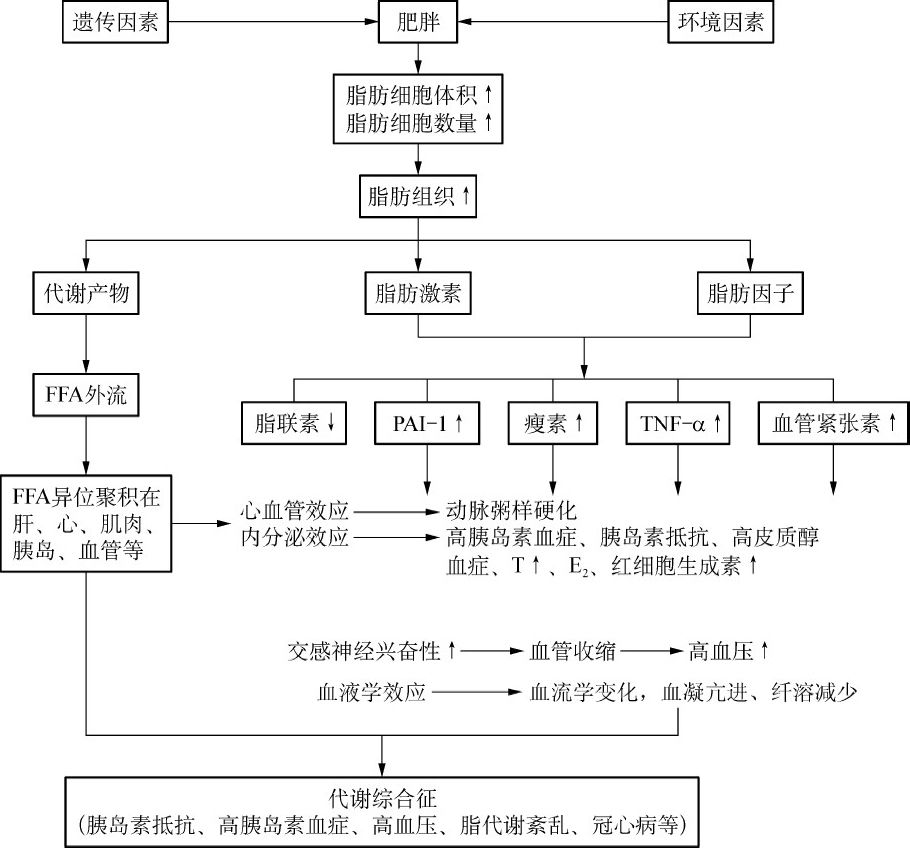
\includegraphics{./images/Image00023.jpg}
 \captionsetup{justification=centering}
 \caption{脂肪代谢产物、激素、细胞因子与肥胖及代谢综合征的关系}
 \label{fig3-1}
  \end{figure} 

\hypertarget{text00004.htmlux5cux23mllj16}{%
\subsection{肥胖病的临床表现}\label{text00004.htmlux5cux23mllj16}}

(一)肥胖病的一般表现

怕热、多汗、易疲劳、关节痛、反应迟钝、活动行走困难、心慌气短等,且易发生自卑、焦虑、抑郁等心理问题。

(二)肥胖病的危害与相关疾病

肥胖将成为21世纪心血管系统疾病的罪魁祸首和严重危害全球人类身心健康的公共卫生健康问题。WHO就肥胖病发生相关疾病的危害见表3-8。

\begin{table}[htbp]
\centering
\caption{肥胖病发生其他疾病的危害度(WHO,1998)}
\label{tab3-8}
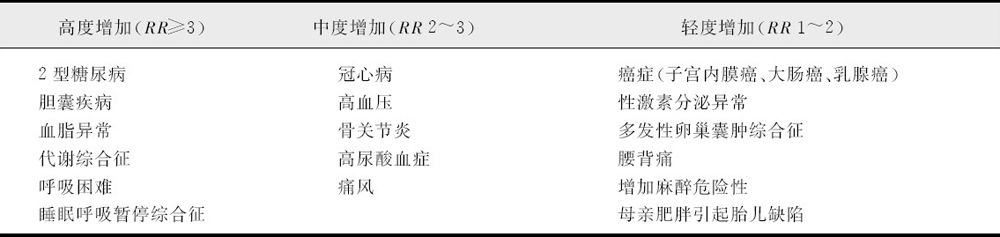
\includegraphics{./images/Image00024.jpg}
\end{table}

\hypertarget{text00004.htmlux5cux23mllj17}{%
\subsection{肥胖病的预防和治疗}\label{text00004.htmlux5cux23mllj17}}

(一)肥胖病的预防

肥胖病是一项生物-心理-社会医学模式的疾病反应。其病因复杂和慢性病程的特点决定了只有采取综合性治疗方案才能达到满意的治疗效果。预防肥胖比治疗更奏效、更有意义。超重者BMI控制在24kg/m\textsuperscript{2}
以下,其可防止人群中40%~50%肥胖相关疾病的危险因素聚集。建立以防为主、防治结合的原则,才是治疗肥胖的根本措施。预防肥胖的具体措施包括以下几个方面。

1.增强和提高合理饮食的观念,学习营养与膳食方面的知识。养成良好的饮食生活习惯。控制总能量的摄入,三大营养素结构比应合理(应清淡饮食)。

2.多吃含膳食纤维多的蔬菜和水果,其可产生饱腹感及延缓糖类吸收而降低餐后血糖;刺激肠壁蠕动,促进排便。

3.每天生活有规律,每天需食用早餐,不吃夜宵。

4.适量增加体育锻炼,如登楼、慢跑、跳绳、游泳等。中、重度肥胖或老年肥胖或有心肺功能不全者或有骨关节炎者,需在医生指导下进行锻炼。

5.轻、中度者每月可减重0.5~1kg,重度或重度以上者每周减重0.5~1kg。应注意定期测量体重以自我监控。

(二)肥胖病的非药物治疗

防治超重和肥胖可降低高血压、糖尿病、脂代谢紊乱及高尿酸血症(痛风)等相关疾病(代谢综合征)的患病率。因此,医学界和社会各类人群应将肥胖当成一种疾病对待,从保护自身健康出发加以控制。

{1.原则}
 肥胖病是一种病因复杂,涉及生化、神经、生理、遗传、环境、文化及社会心理等多方面因素的慢性疾病。因此,肥胖病只有采取综合治疗措施,才能达到满意疗效。

{2.均衡营养治疗的具体方案}

(1)轻度肥胖:只要改变不良的饮食生活习惯及适度的总能量控制,配合适当的运动,就能使体重基本保持或接近正常值范围(见肥胖病的评价指标与诊断)。这个时期治疗十分重要,是预防代谢综合征发生的起始阶段。良好的生活习惯主要指:三餐饮食须规律,避免不吃早餐;三餐能量分配为30%、40%、30%,早餐质量须保证,晚餐能量摄入须控制;避免夜宵习惯;避免油炸等食物。良好的饮食习惯:多食绿叶蔬菜(500g/d);多饮白开水(2000ml/d);少喝或不喝含糖饮料;保证水果摄入(150~250g/d);如脂代谢正常,应每天饮牛奶;荤菜以鱼、虾、瘦肉等为主;在控制总能量摄入的饮食治疗时期,应及时补充多种维生素及微量元素制剂;进餐速度应慢。

(2)中度肥胖:首先需培养良好的生活饮食习惯。治疗期的时间长短及总能量摄入应根据年龄、性别、体力活动(工作量)及肥胖程度个体化制定,女性病人在治疗阶段每天总能量为5021~6276kJ(1200~1500kcal),男性病人为6276~7531kJ(1500~1800kcal),碳水化合物、蛋白质、脂肪比例分别为50%~55%、15%~20%、20%~30%。治疗期一般持续3~6个月。

(3)重度肥胖:营养治疗的具体方案同轻、中度肥胖。治疗期持续时间可根据肥胖程度、脏器功能(肝、肾)等情况适当延长。中、重度肥胖治疗期须注意以下几点:①总能量摄入应适宜:一般不低于5021kJ/d(1200kcal/d),每天能量消耗亏损2092~4184kJ(500~1000kcal),1个月可减重2~4kg。坚持缓慢稳定的个体化营养治疗方案才能保证人体各组织器官功能正常代谢及平衡稳定的内稳态,才能保证有效的不反弹的减重,才能达到防治肥胖病及代谢综合征的目的。②保证蛋白质摄入量:为维持正氮平衡及各组织器官功能正常代谢,应保证摄入足够的优质蛋白质,蛋白质占总能量的15%~20%,如肝、肾功能受损或高尿酸血症或伴痛风,则应适当减少蛋白质总量,以优质蛋白质为主。③及时补充维生素和微量元素:由于限制总能量摄入,使维生素和微量元素的摄入减少。水溶性维生素能促进脂肪分解,对调节脂代谢有重要作用。所以,应及时补充多种维生素和微量元素。

{3.运动治疗}
 成功控制体重的另一个重要因素是增加体力活动。如果单独采用增加体力活动或运动来治疗肥胖,3个月可能有4~5kg体重的减少。体力活动应依年龄和特定文化,强调增加习惯性的日常活动,如步行和爬楼梯。肥胖病人并不必进行高强度活动,轻到中度即已足够。活动强度以轻微出汗、心率增加、自我感觉舒适为宜。心率增加可达到[(170~210)-年龄(岁)]次,举例来说,70岁老人运动后心率可增加到100~140次。活动时间每天至少1小时以上,每天走路1万步以上,有较好的健身效果。

(三)肥胖病的药物治疗

药物治疗只能在改变不良的饮食生活习惯及适度的总能量控制、适当的运动保证下酌情使用,一般适用于重度肥胖者。

减重药物分两大类,即影响中枢神经系统的药物和作用于中枢神经系统以外的药物。

{1.作用于中枢神经系统的药物}
 西布曲明通过抑制5-羟色胺和去甲肾上腺素的再摄取而增加饱腹感和安静状态下的代谢率。其不良反应较少,但有引起血压升高、心率增快、失眠及便秘的报道。

麻黄素和咖啡因作用于去甲肾上腺素旁路的药物,引起厌食和有某些产热作用。高血压和心动过速者不宜使用。

{2.作用于中枢神经系统以外的药物}
 二甲双胍适用于2型糖尿病及糖耐量异常的肥胖病病人。其作用机制尚不清楚,可能与减少肝糖原合成和输出、增加葡萄糖利用及抑制葡萄糖吸收有关。慎用于心功能不全、老年肥胖者及伴肝功能不全者。

奥利司他(塞尼可)是一种胰脂肪酶抑制剂,通过减少脂肪吸收来达到减重目的。该药物作用于肠腔内,基本上不进入血液循环。其不良反应是影响脂溶性维生素吸收,可引起油性大便。

(四)儿童肥胖病的治疗

治疗儿童肥胖病最重要的两点是:①禁用药物治疗;②儿童在不断的生长发育中,其身高在持续增长,维持原有体重即等于减重治疗,实际上其BMI百分位值在下降。应鼓励家属培养儿童良好的饮食及生活习惯,增加儿童运动的时间。总之,应在保证儿童正常生长发育所需能量及营养素的基础上,适当减少能量摄入。极低能量饮食(very
low caloric diet, VLCD)禁用于肥胖儿童。

肥胖病的治疗按经济费用分别占2003年中国卫生总费用和医疗总费用的3.0%和3.7%,近几年还在上升。如全社会各方面对慢性代谢疾病的防治都引起重视,不但能降低全社会医疗费用支出,更重要的是提高全民的生活质量。

\hypertarget{text00004.htmlux5cux23mllj18}{%
\section{ 营养与糖尿病}\label{text00004.htmlux5cux23mllj18}}

糖尿病(diabetes mellitus,
DM)是一组病因和发病机制尚未完全阐明的内分泌-代谢疾病。随着全球经济迅猛发展,人口老龄化、肥胖发病率增高、体力活动不足、膳食不平衡以及应激状态增多等危险因素的迅速增加,糖尿病的发病率逐年上升。据WHO和国际糖尿病联盟(International
Diabetes Federation,
IDF)2007年的统计,目前全球糖尿病病人已超过2.46亿,印度、中国和美国是当今世界上糖尿病病人最多的3个国家。预计2025年DM病人将增至3.33亿,占全球成年人6.3%,增加72%。而据近两年统计,中国的糖尿病病人已近5000万。此外,2型糖尿病在儿童、青少年中的发病率有升高趋势,这与儿童、青少年肥胖人群的增加有关。

糖尿病可以导致多种器官的长期损害,严重危害了人类的健康。WHO有关资料表明,糖尿病的患病率、致残率和病死率以及对总体健康的危害程度,已居慢性非传染性疾病的第3位。糖尿病造成的死亡,已居当今世界死亡原因的第5位。目前,糖尿病等慢性疾病发病率在我国呈上升趋势,而糖尿病的治疗,特别是并发症的治疗已成为个人、家庭和政府的沉重经济负担。因此,为了减轻经济负担、提高全民健康水平,糖尿病及其并发症的综合防治已经受到越来越多的关注,而营养防治是糖尿病防治中最基本、最重要的手段。

\hypertarget{text00004.htmlux5cux23mllj19}{%
\subsection{分型及诊断标准}\label{text00004.htmlux5cux23mllj19}}

(一)定义

糖尿病是一组由于胰岛素分泌和(或)作用缺陷导致的以高血糖为特征的慢性代谢性疾病。糖尿病的长期高血糖状态会引发各种器官特别是眼、肾、神经、心脏和血管等的长期损害及功能障碍甚至衰竭。

(二)分型

按照沿用至今的1999年WHO标准,糖尿病主要分为以下几种类型。

{1.1型糖尿病}  旧称胰岛素依赖型糖尿病(insulin-dependent diabetes
mellitus,
IDDM),是胰岛β细胞破坏导致的胰岛素绝对缺乏。大多起病于儿童及青少年期,占所有糖尿病病人的5%~10%。1型糖尿病通常发病较急、病情较重,需终生依赖外源性胰岛素治疗而存活。

{2.2型糖尿病}  旧称非胰岛素依赖型糖尿病(non-insulin-dependent
diabetes mellitus,
NIDDM)。由胰岛素抵抗背景下的进行性胰岛素分泌缺陷导致的。大多起病于中老年期,但近10年来已有低龄化的趋势。此型糖尿病病人占所有糖尿病病人的90%~95%。2型糖尿病通常起病缓慢、隐匿,大多数此型的糖尿病病人存在肥胖和饮食、生活方式的不合理。至少在其发病初期,甚至于终生都不需要依赖胰岛素治疗而存活。

{3.其他类型}
 由β细胞遗传缺陷、胰岛素作用遗传缺陷、胰腺外分泌疾病(如囊性纤维病)、内分泌疾病、感染等引起的糖尿病;由药物或化学制剂诱发的糖尿病(如AIDS治疗后或器官移植后);罕见的免疫介导的糖尿病以及其他与糖尿病相关的遗传综合征。

{4.妊娠糖尿病}
 妇女在妊娠期间出现或发现的任何程度的葡萄糖耐受不良,占妊娠妇女的1%~14%。大部分病人分娩后可恢复正常,但可能增加今后发生糖尿病的危险性。

{5.糖耐量受损(impaired glucose tolerance,
IGT)和空腹血糖受损(impaired fasting glucose, IFG)}
 一群处于中间状态的人群,其血糖水平升高,虽未达到糖尿病诊断标准,但也不能归为正常。美国糖尿病协会(American
Diabetes Association,
ADA)将IFG和IGT命名为“糖尿病前期”,而IDF则将其统称为“中间高血糖”。IFG和IGT均为糖尿病和心血管疾病的危险因素。

(三)诊断标准

{1.糖尿病的诊断标准}  见表3-9。

\begin{table}[htbp]
\centering
\caption{糖尿病的诊断标准(WHO,1999)}
\label{tab3-9}
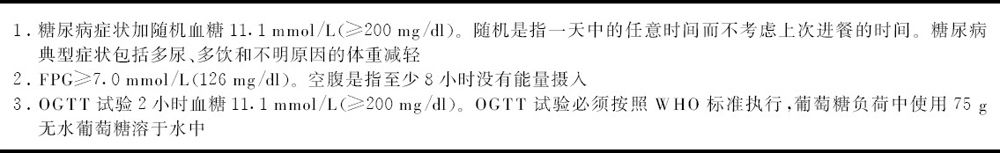
\includegraphics{./images/Image00025.jpg}
\end{table}

注:如果没有出现明确的高血糖,应该另选一天对这些评判指标进行一次重复试验加以确认。第3次OGTT试验的结果不作为常规临床考虑。

{2.IGT和IFG的诊断建议}  见表3-10。

\begin{table}[htbp]
\centering
\caption{IGT和IFG的诊断建议(WHO/IDF,2006)}
\label{tab3-10}
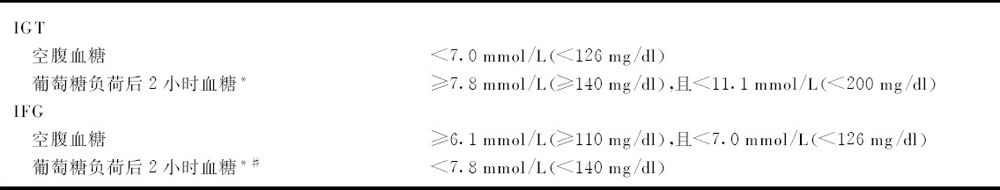
\includegraphics{./images/Image00026.jpg}
\end{table}

注:*口服75g葡萄糖负荷后2小时血浆葡萄糖;#如果未检测2小时血浆葡萄糖,则糖耐量状态无法确定,不能排除糖尿病或IGT。

\hypertarget{text00004.htmlux5cux23mllj20}{%
\subsection{糖尿病的病因和发病机制}\label{text00004.htmlux5cux23mllj20}}

糖尿病的病因和发病机制较为复杂,至今仍未完全阐明,不同类型糖尿病的病因和发病机制各异,但目前认为主要与遗传因素、环境因素和免疫机制有关。

(一)病因

1型和2型糖尿病的基本病因有两种,即遗传因素和环境因素。遗传因素是基础和内因,而环境因素则是条件和外因。1型糖尿病与第6号染色体短臂的组织相容性抗原(HLA)的复合物异常有密切关系,可以表现出对糖尿病的易感性,此为遗传因素的作用;环境因素则可能是某些对β细胞具毒性的药物和化学物质的摄入、感染等,尤其是病毒如柯萨奇B\textsubscript{4}
病毒的感染,诱发自身免疫,使胰腺分泌胰岛素的β细胞遭到严重甚至永久性的破坏,无法正常分泌胰岛素。同样,2型糖尿病也是遗传因素和环境因素长期共同作用的结果。其遗传倾向更明显、复杂,包括一些基因的突变或表达异常,导致β细胞功能缺陷和胰岛素抵抗;环境因素主要包括肥胖、少活动、糖刺激、外伤或过多使用升高血糖的激素等。

(二)发病机制

糖尿病发病机制复杂,从胰岛β细胞的自身免疫性损伤导致的永久性胰岛素缺乏,到胰岛素抵抗所致的胰岛素作用异常,都有涉及。

{1.1型糖尿病的发病机制}
 主要是在遗传因素的控制下,环境因素对β细胞产生直接毒性作用、提高β细胞对损伤的易感性或者启动自身免疫反应等。较为关键的环节是胰岛β细胞的渐进性破坏,其中90%由细胞免疫介导。这种自身免疫反应使90%新发病的糖尿病病人循环血中出现自身抗体,如抗胰岛细胞抗体(islet
cell antibodies, ICA)、胰岛素自身抗体(insulin autoantibodies,
IAA)、谷氨酸脱羧酶(glutamic acid decarboxylase,
GAD)抗体以及酪氨酸磷酸酶抗体IA-2α和IA-2β等。各种自身抗体通过细胞介导的免疫反应导致胰岛β细胞的进行性破坏。同时,1型糖尿病还普遍存在胰岛炎症,T细胞、B细胞、巨噬细胞、粒细胞和NK细胞均参与了炎症反应。胰岛炎症的发生使胰岛β细胞的功能逐渐丧失,数目逐渐减少,胰岛素的分泌也逐渐减少,血胰岛素绝对含量降低,从而导致糖尿病的发生。

{2.2型糖尿病的发病机制}  主要是由胰岛素分泌缺陷和胰岛素抵抗所致。

(1)胰岛素分泌缺陷:胰岛素是由胰岛β细胞产生和分泌的,并调节体内三大营养素代谢,尤其是糖代谢的主要激素。葡萄糖是胰岛素作用的底物,也是调节胰岛素分泌的主要物质。生理状态下,进食后引起血糖升高,通过一系列生化反应使β细胞发生胞吐作用,胰岛素被释放。胰岛素的分泌可分为3个阶段,其中第一时相胰岛素分泌可高达基础值的10倍,又称快速分泌相;第二时相则分泌量远大于第一时相;第三时相是当血糖降至正常,胰岛素分泌也回到基础水平。

糖尿病病人由于胰岛β细胞功能衰退,胰岛素分泌的第一时相减弱或消失,为维持正常血糖,β细胞增生、肥大、代谢活跃,处于代偿阶段,此时空腹和餐后血糖均可以维持正常。之后,随着β细胞功能的进一步下降,胰岛素分泌正常或高于正常,但不能应对餐后等高血糖状态,出现了糖耐量受损。而当确诊为糖尿病时,β细胞的功能已仅为正常时的50%。发展到晚期,β细胞功能衰竭,完全失去代偿,进一步加重胰岛素抵抗和胰岛损伤,机体长期处于高血糖状态并引起全身并发症。

(2)胰岛素抵抗:胰岛素抵抗是指组织对胰岛素的反应性降低,是2型糖尿病的早期重要特征之一,可导致血糖升高,被认为是2型糖尿病的发病机制之一。

引起胰岛素抵抗的原因有很多,包括血胰岛素抗体的产生、各种原因造成的胰岛素受体和胰岛素信号转导系统中各信号分子的数量、结构和功能的破坏等,都可能导致胰岛素抵抗。影响组织对胰岛素反应性减低的因素有:①胰岛素抗体使能与组织结合的胰岛素量减少,胰岛素的生物学效应降低;②胰岛素受体自身抗体和高胰岛素血症引起胰岛素受体下调,两者均导致细胞膜上胰岛素受体数量减少,细胞对胰岛素的反应性降低;③外周靶器官对胰岛素反应性降低和某些激素过多造成的胰岛素抵抗,前者主要包括肥胖、肝脏疾病和肌无力,后者包括糖皮质激素、生长激素、儿茶酚胺等。

近年有研究显示,炎症在胰岛素抵抗和胰岛β细胞损伤的发生过程中起了非常重要的作用。目前,2型糖尿病被认为是一种慢性炎症疾病,胰岛素抵抗是一个慢性非特异性炎症的持续过程,在此过程中血液和(或)组织中的单核细胞、巨噬细胞等炎症细胞产生炎症因子,肝组织产生急性反应物质。近来发现,异位脂肪组织细胞也处于一种慢性炎症状态,也可分泌许多脂肪因子和炎症因子,包括瘦素、脂联素、肿瘤坏死因子-α(TNF-α)、白细胞介素-1(IL-1)、白细胞介素-6(IL-6)、干扰素-γ(IFN-γ)等。这些脂肪因子和炎症因子干扰胰岛素IRS/PI3K信号传导通路,是炎症导致胰岛素抵抗的主要分子机制。

(三)膳食、生活方式因素

研究表明,环境因素在2型糖尿病的发生中起着很重要的作用,膳食是主要的环境因素之一,膳食类型已有重大改变,运动减少、超重和肥胖增加使糖尿病增加非常显著。改变膳食类型的特点是典型的高能量、高饱和脂肪酸、极少纤维素(或非淀粉多糖)。这种膳食特点与高空腹血糖和高胰岛素、葡萄糖耐量减低(IGT)和IGT进展与糖尿病患病率增加有联系。大规模的人群研究已证实不良的生活方式和行为是促使2型糖尿病发生和发展的主要途径之一,多年来的研究表明膳食中一种或几种营养素与2型糖尿病关系密切。

{1.高脂膳食}
 研究表明,2型糖尿病(NIDDM)的发生率与膳食脂肪所提供的能量百分比呈正相关。含高饱和脂肪的膳食早已被证明可增高血总胆固醇和低密度脂蛋白胆固醇水平,并可引起胰岛素的抵抗作用。Feskens等在荷兰进行的纵向流行病学研究指出饱和脂肪酸及胆固醇的摄入与空腹血糖水平呈明显正相关,不仅具有增高血脂水平、降低糖耐量,及增加胰岛素抵抗的作用,而且还具有增加体重、改变体脂分布的影响,从而增加了糖尿病发病的危险性。大量的流行病学调查也证实,总脂肪和饱和脂肪酸的摄入量与糖尿病发生的危险性呈正相关。调查发现,生活在美国的第2代日裔男性膳食结构与美国人相似,摄入的脂肪占总能量的32.4%,而日本本土男性摄入脂肪占16.7%;流行病学调查发现,前者糖尿病的患病率是后者的4倍,两者有显著差异。Marshall等人对1317人进行的前瞻性队列研究中,发现每天多摄入40g脂肪,患糖尿病和糖耐量减低的危险度分别增加1.51倍和1.62倍。印第安式的饮食为传统的低脂肪、高碳水化合物、高膳食纤维食物,英国人的饮食为典型的美式高脂肪、低碳水化合物饮食,经过几年的观察发现:英国人膳食结构人群糖尿病发病是两种膳食都采用的混合式的2.5倍,而混合式膳食结构人群糖尿病发病是印第安式的1.3倍,结论为英国人膳食结构可能增加Pima地区的印第安人发生糖尿病的危险;美国卫生专业人士随访研究发现饱和脂肪酸摄入增加与2型糖尿病的发生呈正相关,经常摄入成品肉可以增加糖尿病的发生率。

通过动物实验发现,采用高脂低碳水化合物会导致实验动物糖耐量减低及葡萄糖刺激后的胰岛分泌减少,同时血浆游离脂肪酸浓度升高。研究中还发现,即使严格限制能量摄入,高脂低碳水化合物饮食同能量过多摄入一样,可抑制胰岛素分泌及减低胰岛素敏感性。进一步研究的结果证实,长期高脂低碳水化合物饮食可抑制胰岛素分泌,降低胰岛素敏感性,导致糖尿病的发生。美国夏威夷的日本移民的2型糖尿病的患病率比日本广岛的日本人高出1倍多,这两组人群的膳食总能量摄入相似,但夏威夷日本人的复合碳水化合物的摄入比广岛日本人少1/3,而脂肪摄入则高出1倍。由此可见,高脂低碳水化合物的饮食是糖尿病和糖耐量减低发生率增高的重要原因之一。

{2.蛋白质}
 美国研究人员发现人体内某些蛋白质的缺陷能够影响胰脏及肝脏中基因的功能。据美国《科学》杂志报道,马萨诸塞州怀特黑德生物医学研究院的研究人员在仔细研究整个人类基因组后发现,一些蛋白质中存在的缺陷会导致常发生于成年人的2型糖尿病。我国研究发现,在胚胎发育期,低蛋白膳食易导致胰腺发育不良和β细胞功能缺陷,增加了成年后发生2型糖尿病的危险。King等提出在那些存在着持续性或周期性蛋白质缺乏或不规则供给的地区,2型糖尿病的发病率也高,提示蛋白质的缺乏与2型糖尿病的发病存在着一定的相关性。研究发现胚胎期母体摄入的蛋白质不足,会出现胰岛发育不良,β细胞减少可出现其功能减弱,甚至造成β细胞不可修复的损伤,增加成年后出现糖尿病的危险性。在摄入能量相等的情况下,低蛋白摄入组的胎鼠胰腺β细胞数目、胰岛的大小、增殖能力和胰腺中胰岛素的水平明显较对照组低。

流行病学调查发现,糖尿病也常出现在较贫穷的地区,推测这种现象可能与母亲怀孕期间饮食缺乏蛋白质有关。临床研究显示:出生时体重<2.5kg的婴儿和1岁时<8kg的幼儿,在64岁时,45%以上的人患糖尿病和心血管系统疾病。加拿大渥太华医学专家斯高特等研究发现,小麦所含的一种名为GIBI的蛋白质会影响某些幼儿的免疫系统,从而引发糖尿病;还发现,当幼儿的免疫系统攻击小麦所含的这种蛋白质后,还会继续攻击胰腺分泌胰岛素的细胞,最终将分泌胰岛素的细胞杀死,从而引发糖尿病。

{3.微量元素}

(1)铬:研究发现,铬(Cr)缺乏可引起空腹高血糖、葡萄糖耐受削弱、胰岛素受体数减少及外围神经性疾病等。铬是胰岛素的一种“协同激素”(cohormone),作为胰岛素的增敏剂参与并影响糖、脂肪和蛋白质的代谢。因此,胰岛素在体内发挥作用时需要铬的参与,而葡萄糖耐受因子(GTF)也只能在胰岛素存在的情况下,才能发挥生化效应。众多的临床和实验资料认定,铬是能够增强胰岛素作用的微量元素,当血中铬减少时,糖耐量受损,组织对胰岛素的敏感性降低,严重时会出现尿糖。

Schwar等发现GTF的活性组分主要是3价铬离子(Cr\textsuperscript{3+}
)。其证据主要有以下4个方面:①给大鼠喂食低铬的含糖饮食,这些大鼠相继出现高胰岛素血症和高脂血症,葡萄糖耐受实验中胰岛素曲线下的面积增加,表明这些大鼠患了胰岛素抵抗。②给5位病人全胃肠外营养静脉注射(TPN)不含铬的营养剂,相继出现2型糖尿病等症状,补铬后症状消失。③血清葡萄糖的增加伴随着尿铬排泄的增加,当葡萄糖代谢的条件发生改变,尿铬的排泄也随之改变。例如Clodfelder等发现糖尿病大鼠的尿铬损失比对照组大,血清铬含量低。Ghosh等在对50例印度2型糖尿病病人的研究中也发现糖尿病病人的血清铬水平比健康对照组低(32.3nmol/L对44.7nmol/L,
P<0.001)。Morris等发现2型糖尿病病人的血清铬水平只有健康人的1/3,尿铬水平则比健康人高2倍。我国糖尿病病人血清铬含量也明显低于健康对照组,且与病程、血糖、三酰甘油及胆固醇水平呈负相关。④人对铬的吸收和饮食中铬摄入量呈负相关(大鼠例外),例如摄取10μg时吸收率约为2%,但摄取40μg时吸收率减少到0.5%。这些研究结果表明,铬和葡萄糖代谢,也许和胰岛素功能之间存在着一定的联系。

(2)锌:国内外有关糖尿病病人血锌的测定结果不一,大部分报道降低。锌与胰岛素的合成、分泌、贮存、降解、生物活性及抗原性有关。锌主要分布在胰岛β细胞的分泌颗粒中,促使胰岛素结晶化,锌激活羧化酶使胰岛素原转变为胰岛素,并提高胰岛素的稳定性。胰岛素是体内降低血糖的唯一激素,它的分子构造中有2个金属原子锌,缺锌的胰岛素易变性失效,从而影响葡萄糖在体内的平衡过程。李少旦等在对“糖尿病病人血清微量元素的含量分析”中发现,糖尿病病人血清锌水平降低,且与对照组相比有显著差异(P<0.01)。缺锌可诱导产生胰岛素抵抗,使胰岛素生成下降,易并发糖尿病。动物试验表明,缺锌的大鼠体内羧肽酶β活性下降50%,无活性的胰岛素原转变为有活性胰岛素的趋势下降,从而造成血清胰岛素水平下降。Juturu等研究发现,糖尿病病人普遍缺锌,几种糖尿病并发症也与细胞锌或锌依赖抗氧化物酶的降低有关。

(3)硒:许多研究证实,糖尿病病人因葡萄糖和糖基化蛋白质自动氧化等可产生大量自由基,同时机体抗氧化物质如抗氧化酶活性下降,对自由基清除能力减弱,从而产生明显的氧化应激,而硒缺乏时机体对氧化损伤的敏感性增加,过多的自由基积累则可引发生物膜磷脂中不饱和脂肪酸的一系列自由基反应,即脂质过氧化,可导致:①膜的流动性发生不可逆的改变,脆性增加;②与膜结构相联系的胰岛素受体受到不同程度的影响,从而减弱与胰岛素的结合;③毛细血管基膜的脂质过氧化可使基膜通透性增高。这些改变是糖尿病时葡萄糖代谢障碍和发生微血管病变的重要机制。研究表明,缺硒引起胰岛损伤的主要变化是以β细胞为主体的结构与功能的异常。动物实验结果显示,大鼠通过补硒后,糖、脂代谢紊乱得到了一定的改善,超氧化物歧化酶(SOD)、谷胱甘肽过氧化物酶(GSH-Px)活力明显提高,MDA水平下降,说明硒通过提高抗氧化系统的防御功能对抗了自由基对胰岛β细胞的损害,在一定程度上保护了胰岛的β细胞,改善了糖尿病大鼠的胰岛功能及物质代谢的紊乱。糖尿病病人的临床表现与病人体内硒水平有密切关系。据杨辉等报道,糖尿病病人治疗前血清硒明显降低,且与血糖呈负相关,血清硒降低必然会影响GSH-Px活性,加重了胰岛细胞的损伤和血管神经病变的发生、发展。

{4.超重/肥胖与腰围}
 体重超重/肥胖和腹部脂肪蓄积是2型糖尿病发病的重要危险因素。我国24万人群数据的汇总分析显示,如以空腹血糖≥126mg/100ml或餐后2小时血糖仍≥200mg/100ml者诊断为2型糖尿病病人,BMI≥24者的2型糖尿病的患病率为BMI<24者的2.0倍,BMI≥28者的2型糖尿病患病率为BMI<24者的3.0倍。男性和女性腰围分别为≥85cm和≥80cm时,糖尿病的患病率都为腰围正常者的2~2.5倍。肥胖病人的胰岛素受体数减少和受体缺陷,发生胰岛素抵抗(对胰岛素不敏感)现象和空腹胰岛素水平较高,影响到对葡萄糖的转运、利用和蛋白质合成。中心型脂肪分布比全身型脂肪分布的人患糖尿病的危险性更大;肥胖持续的时间越长,发生2型糖尿病的危险性越大。儿童、青少年时期开始肥胖,18岁后体重持续增加和腹部脂肪堆积者患2型糖尿病的危险性更大。腰围超标、血清三酰甘油和低密度脂蛋白胆固醇升高、高密度脂蛋白胆固醇降低、血压升高和空腹血糖异常高等危险因素中,如出现多个因素聚集,即临床上定义的代谢综合征,有很强的致动脉粥样硬化作用。代谢综合征与胰岛素抵抗密切相关,肥胖、腰围超标和缺少体力活动是促进胰岛素抵抗进展的重要因素。

Jonathan等对加拿大埃德蒙顿地区一所学校875名5~19岁的儿童进行调查发现,根据BMI确定的肥胖和超重的患病率分别为7.8%和14.3%。美国Liu等对青少年糖尿病病人调查资料分析发现,超重患病率为非西班牙裔白人94.7%,非西班牙裔黑人100%,西班牙裔青少年90.5%。在非西班牙裔白人青少年1型糖尿病病人中超重的患病率和风险率分别为11.9%和21.5%;在非西班牙裔黑人分别为31.9%和23.6%;在西班牙裔分别为18.3%和28.5%。与健康同龄人相比,青少年2型糖尿病病人更多合并超重,而青少年1型糖尿病病人较少合并超重。与青少年非糖尿病者相比,青少年1型糖尿病病人超重的发病率与之相当,但发生超重的危险性增高。

\hypertarget{text00004.htmlux5cux23mllj21}{%
\subsection{糖尿病病人的营养代谢变化}\label{text00004.htmlux5cux23mllj21}}

(一)碳水化合物代谢

胰岛素在人体内的重要功能包括传送葡萄糖和氨基酸、制造肝糖原,将葡萄糖转化成三酰甘油、合成核酸及蛋白质。血糖是刺激胰岛素分泌最重要的因素。由于胰岛素与其受体结合后才发挥作用,所以胰岛素的分泌量及其受体数目均与糖尿病发生有密切关系。当胰岛素不足时,肝脏摄取葡萄糖合成糖原的能力减弱,使过多葡萄糖进入血液循环,组织利用葡萄糖的能力减弱,空腹及餐后肝糖输出增加;又因葡萄糖异生底物的供给增多及磷酸烯醇型丙酮酸羧基酶活性增强,肝糖异生增加,因而出现空腹及餐后高血糖。血糖升高可引起全身性的代谢紊乱,造成一系列急性并发症,并在蛋白糖化及糖尿病慢性并发症的形成中起重要作用。此外,高血糖还将严重影响β细胞的功能,是引起胰岛β细胞功能损害、糖尿病病情恶化的重要因素,也称高血糖毒性作用。通过饮食疗法、运动疗法及适当药物尽可能使血糖维持在一个接近正常的水平是维持及恢复β细胞功能的一个重要措施。

(二)脂肪代谢

正常人体脂肪代谢处于动态转化过程中,糖尿病病人胰岛素不足,体内脂肪组织摄取葡萄糖及从血浆清除三酰甘油的能力下降,脂肪合成减慢、分解加速,血浆游离脂肪酸水平升高。当胰岛素极度缺乏时,激素敏感性脂酶活性增强,储存脂肪的动员和分解进一步加速。而分解产生的大量三酰甘油及游离脂肪酸,经β氧化而生成大量乙酰辅酶A,又因糖酵解生成草酰乙酸减少,使乙酰辅酶A不能与草酰乙酸充分结合进入三羧酸循环氧化为能量,因而大量缩合成乙酰乙酸,进而转化为丙酮和β-羟丁酸,即产生大量酮体。当酮体生成过速,超过组织利用和排泄能力时,在体内大量堆积而造成酮症,进一步可发展至酮症酸中毒。此外,糖尿病病人由于胆固醇的合成旺盛还会形成高胆固醇血症,而血中三酰甘油增多则是糖尿病微血管病的重要发病因素。与高血糖毒性作用相似,血脂异常如果不加以纠正,会引起β细胞功能的进行性下降。

(三)蛋白质代谢

由于糖代谢异常造成能量来源不足,为了补充能量,部分蛋白质氧化分解;同时,糖尿病病人肝、肌肉等组织摄取氨基酸也减少,蛋白质合成代谢减弱、分解代谢加速,这些因素均导致负氮平衡。血浆中成糖氨基酸(甘氨酸,丙氨酸,苏氨酸和谷氨酸)浓度降低,提示糖异生旺盛,成为肝糖输出增加的主要来源;成酮氨基酸(亮氨酸、异亮氨酸和缬氨酸等支链氨基酸)浓度升高,反映肌肉组织摄取这些氨基酸合成蛋白质能力降低,导致病人乏力、消瘦、组织修复和抵抗力降低、儿童生长发育障碍和延迟。此外,蛋白质代谢紊乱还会影响免疫球蛋白产生,故糖尿病病人细胞及体液免疫能力减低,易发生各种感染并可能出现伤口不愈。儿童发生糖尿病,生长发育会因蛋白质分解而受阻,抵抗力相应减弱。

\hypertarget{text00004.htmlux5cux23mllj22}{%
\subsection{糖尿病的临床表现与并发症}\label{text00004.htmlux5cux23mllj22}}

(一)临床表现

糖尿病的典型症状为“三多一少”,即多饮、多尿、多食和体重下降。由于血糖升高超过肾糖阈,大量葡萄糖从尿中排出,形成高渗性利尿,24小时尿量可达2~10L。体内脱水刺激口渴中枢,引起多饮。胰岛素的相对或绝对不足使体内葡萄糖不能利用,脂肪和蛋白质的分解代谢增加,体重减轻可达10kg以上。体内细胞处于饥饿状态,故造成多食。除此之外,还可能出现疲乏,劳累,视力下降,皮肤瘙痒,手、足麻木,伤口愈合缓慢,反复感染,男性阳痿等不典型症状。

1型糖尿病起病时“三多一少”症状常较明显。但大多数病人,特别是2型糖尿病病人症状常常不明显或发病初期无异常表现。此外,糖尿病的不典型症状往往在其他非糖尿病的情况下也可出现,容易被忽略。以上两种情况都极易导致漏诊。因此对高危者应进行糖尿病和糖尿病前期筛查。

(二)并发症

{1.急性并发症}

(1)糖尿病酮症酸中毒(diabetic ketoacidosis,
DKA):是最常见的急性并发症之一,常见于1型糖尿病病人。感染、胰岛素治疗中断或不当减量、饮食不当、创伤、手术等都可能是其发生的诱因。病人酮体生成量剧增,在血中积聚产生酮症,继而发生代谢性酸中毒,同时机体出现严重失水和电解质紊乱。病人表现为高血糖、脱水、尿量减少、呼吸深快、呼出气体带有烂苹果味(丙酮)、血压降低等,严重者出现昏迷并危及生命。

(2)糖尿病非酮症性高渗性昏迷:多见于中老年2型糖尿病病人,机体内尚有胰岛素分泌,可抑制脂肪分解但利用葡萄糖不够。常见诱因有感染、急性胃肠炎、胰腺炎、脑血管意外、暴饮暴食、某些药物(如肾上腺皮质激素、噻嗪类利尿药等)的应用等。起病早期可出现多尿、多饮,但症状可能不明显。以后失水随病情进展逐渐加重,表现为严重脱水、出现神经精神症状如嗜睡、幻觉、定向障碍、癫痫
样抽搐等,神志不清最后陷入昏迷。此并发症病死率高,应引起高度重视。

(3)低血糖:糖尿病病人,如果应用口服降糖药或胰岛素过量、耽误进餐或食物摄入量不足、运动量加大以及空腹饮酒时,均可能发生低血糖。临床上表现为一系列交感神经兴奋(出汗、心慌、面色苍白、四肢颤抖、饥饿感、软弱无力等)和中枢神经系统功能紊乱(意识模糊、头痛、头晕、言语障碍、幻觉、精神病样发作、痴呆,甚至昏迷等)的症候群。一般情况下,将静脉血浆葡萄糖浓度<2.8mmol/L(50mg/dl)定义为低血糖,但须注意的是,糖尿病的低血糖是体内胰岛素的相对过量,不同病人以及同一病人不同情况下出现低血糖症状时的血糖水平都是不同的。持续的低血糖除可危及生命外,还可导致脑功能障碍,增加心、脑血管意外的危险性。治疗可迅速口服葡萄糖或含糖食品、注射葡萄糖,必要时使用胰高血糖素。

(4)感染:糖尿病常引起皮肤化脓性感染,如疖、痈等;皮肤真菌感染,如足癣;尿路感染,如肾盂肾炎、膀胱炎、肾乳头坏死;女性糖尿病病人常并发真菌性阴道炎、巴氏腺炎等。

{2.慢性并发症}
 糖尿病的发生与体内胰岛素绝对或相对不足有关,由此会引起全身代谢及酸碱平衡失调。随着时间推移,血糖控制不良会导致慢性并发症的陆续出现,这是造成糖尿病死亡的主要原因。

(1)大血管病变:糖尿病可致大、中动脉粥样硬化,它主要侵犯主动脉、冠状动脉、脑动脉、肾动脉和肢体外周动脉,引起冠心病、缺血性或出血性脑血管病、肾动脉硬化、肢体动脉硬化等。肢体外周动脉粥样硬化常以下肢动脉病变为主,表现为下肢疼痛、感觉异常和间歇性跛行,严重供血不足可导致肢体坏疽。

(2)微血管病变

1)糖尿病肾病:糖尿病会诱发肾小球微血管病变、肾动脉硬化和反复或慢性肾炎等肾脏病变,发生率在20%~40%。其特点是大量蛋白尿、肾小球滤过率(GFR)下降和高血压。临床上一般可分为五期(表3-11)。Ⅰ期:肾小球高滤过期;Ⅱ期:间断白蛋白尿期;Ⅲ期:早期糖尿病肾病期;Ⅳ期:临床糖尿病肾病期;Ⅴ期:肾功能衰竭期。其中,Ⅰ、Ⅱ期无明显症状;Ⅲ期开始出现微白蛋白尿,是预防进一步发展的关键时期,如无法逆转即进入Ⅳ期,出现持续蛋白尿;Ⅴ期即终末期最终发生肾衰竭。有些病人往往在尚未出现蛋白尿时已有肾小球滤过率的下降,因此,现在ADA的糖尿病诊疗标准中也采用慢性肾脏病(chronic
kidney disease, CKD)分期(表3-12),即基于肾小球滤过率评估结果的分期。

\begin{table}[htbp]
\centering
\caption{糖尿病肾病临床分期和临床表现}
\label{tab3-11}
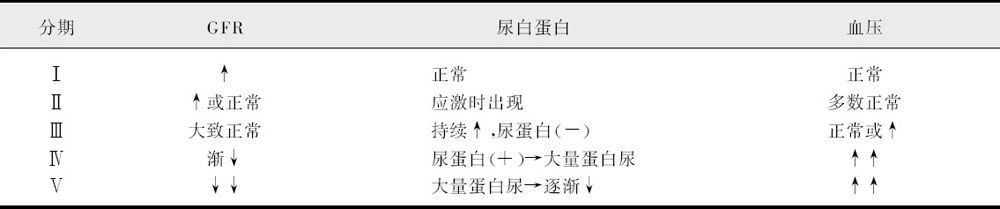
\includegraphics{./images/Image00027.jpg}
\end{table}

\begin{table}[htbp]
\centering
\caption{CKD分期}
\label{tab3-12}
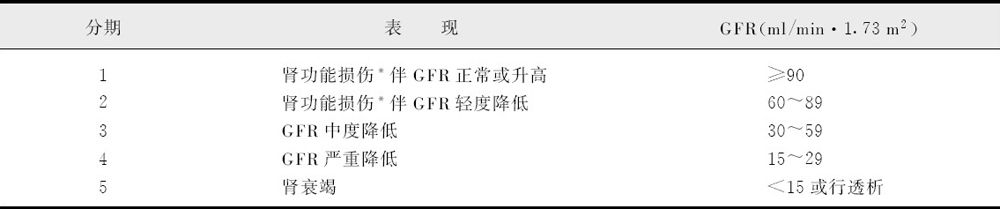
\includegraphics{./images/Image00028.jpg}
\end{table}

注:*肾功能损伤包括病理学、尿液学、血液学或影像学试验异常。1.73m\textsuperscript{2}
指体表面积。

2)糖尿病视网膜病变:是微血管病变的又一重要表现。主要改变包括视网膜微血管瘤、出血斑、渗出、新生血管、视网膜前和玻璃体出血、视网膜剥离等。致盲的概率显著高于正常人。

(3)神经病变:病变部位以周围神经为主,通常为对称性,下肢较上肢严重,病情进展缓慢,临床上先出现肢端感觉异常、肢痛、肌力减弱甚至肌萎缩和瘫痪等。自主神经病变也较常见,且较早出现,影响胃肠、心血管、泌尿系统和性器官功能。

(4)糖尿病足:糖尿病病人由于末梢神经病变、下肢动脉供血不足,以及细菌感染等多种因素,引起足部疼痛、皮肤深溃疡、肢端坏疽等病变,统称为糖尿病足,是糖尿病最常见的并发症之一,严重者可能需要截肢或发生死亡。2005年“世界糖尿病日”的主题即为“关注糖尿病足”,宣传对糖尿病足的早期预防和治疗,以降低其致残率和致死率。

\hypertarget{text00004.htmlux5cux23mllj23}{%
\subsection{糖尿病的综合治疗原则}\label{text00004.htmlux5cux23mllj23}}

早在半个多世纪以前,美国著名糖尿病专家就曾把糖尿病的治疗比作是驾驭一辆三匹马的战车,这三匹战马分别是饮食治疗、胰岛素治疗(当时尚无口服降糖药)和运动治疗,精辟地提出了糖尿病的综合治疗原则。近年来,根据实践经验的总结,公认的糖尿病综合治疗原则包括以下5条:①糖尿病的教育与心理治疗;②糖尿病饮食治疗;③糖尿病运动治疗;④糖尿病药物治疗;⑤糖尿病的病情监测。只要认真掌握好这5条原则,就能使糖尿病获得良好的控制,避免或延缓急、慢性并发症的发生和发展。

(一)糖尿病的教育与心理治疗

{1.糖尿病的教育}

(1)糖尿病教育的意义:糖尿病是一种终身性的疾病,但通过适当的治疗措施可以被良好控制。为了达到这一目标,医务工作者应使糖尿病病人了解该疾病的基本知识,学会维持生命的基本技能和控制疾病的方法,达到自我控制病情、自我保健的目的。由此,糖尿病教育日趋受到全世界的关注。良好的糖尿病教育可提高病人自我血糖控制和调节能力,减少和延缓并发症的发生和发展,降低住院率,减少药物用量,从而直接减少病人和社会的经济负担。而就我国目前情况而言,糖尿病的发病率高,而糖尿病教育体系则尚欠完整,专职糖尿病教育人员偏少,大力开展糖尿病教育、探索符合国情的糖尿病教育模型和体系已迫在眉睫。

(2)如何进行糖尿病教育:可以建立一个糖尿病治疗和健康教育小组,定期进行糖尿病教员培训并设计教育课程,采用生动多样的健康教育形式使糖尿病病人正确认识自己的疾病和病情,改变错误观念;掌握药物或胰岛素的使用和饮食计划的设计;学会血糖自我监测。此外,还应建立系统性的社会教育网,由政府直接参与对糖尿病教育的组织和调控。糖尿病教育应该贯穿糖尿病病人的一生。

{2.糖尿病的心理治疗}
 随着近年来生物---心理---社会医学模式的提出,给糖尿病的研究带来了一种新的思路。研究发现,如工作学习长期过度紧张、人际关系不协调、生活中的突发不幸事件等社会、心理上的不良刺激,都可能是糖尿病发生和加重的影响因素,认识到糖尿病也是身心疾病的一种,治疗糖尿病也必须重视纠正和消除来自社会、环境的不良刺激,使不正常的心理状态恢复正常。因此,心理治疗也是一个不能忽略的重要环节。

(二)糖尿病的饮食治疗

在糖尿病的发生和发展中,饮食因素起着相当重要的作用。因此,饮食治疗是糖尿病治疗的基础,在后节将会详细叙述。

(三)糖尿病的运动治疗

对于2型糖尿病,运动和饮食是一切治疗的基础和保障;对于1型糖尿病来说,最根本的原则是保持饮食、运动和胰岛素作用三者的平衡与统一。由此可见,运动在糖尿病治疗中的重要地位。通过适当的、长期不懈的体育锻炼,可以有助于使肥胖病人体重减轻、对胰岛素的敏感性增强,使血糖得到良好的控制;对于轻型糖尿病病人,还可以改善末梢组织对糖的利用从而使血糖下降,对防止血管、神经并发症都有一定作用。ADA
2007年糖尿病诊疗标准中建议,糖尿病病人每周至少进行中等强度有氧体力活动150分钟(50%~70%最大心率)和(或)每周至少90分钟强度较大的有氧运动(>70%最大心率),以改善血糖控制,帮助保持体重和减少心血管疾病危险。体力活动每周至少3天,且不得连续2天不活动。对无禁忌证的2型糖尿病病人鼓励每周进行3次耐力运动。美国运动医学院专家认为耐力运动可以改善胰岛素敏感性。运动治疗的过程中,必须注意定时、定量、坚持;根据实际情况选择合适的运动方式和运动强度;并且注意预防运动时低血糖的发生。

(四)糖尿病的药物治疗

单纯饮食及运动治疗并不能使所有糖尿病病人的血糖维持在基本正常水平,所以当病程进展到一定程度,甚至在病程早期就应该选用合适的口服降糖药或胰岛素,并根据临床需要,服用降压、调脂等其他药物。

{1.口服降糖药物}
 常用的口服降糖药主要包括以下几类:①磺脲类:可以刺激胰岛素的分泌,分为长效(如格列本脲)、中效(如格列齐特)、短效(如格列吡嗪)以及新一代的格列美脲等;②双胍类:可以降低食欲、减少吸收,适合肥胖病人服用,如二甲双胍等;③α-糖苷酶抑制剂:能使多糖或者双糖降解为单糖的速度减慢以延缓吸收,达到降低血糖的目的,如阿卡波糖、倍欣等;④噻唑烷二酮类(TZDs):为胰岛素增敏剂,能在多种层次上增强胰岛素的敏感性,减少胰岛素抵抗,如罗格列酮和匹格列酮等;⑤格列奈类:为新型短效胰岛素促泌剂,如瑞格列奈、那格列奈等;⑥胰高血糖素样肽-1(GLP-1)类似物:可以刺激胰岛素释放、抑制胰高血糖素、抑制胃酸分泌,如GLP-1激动剂exendin-4等。

{2.胰岛素}
 以下病人需要用胰岛素来控制血糖:①1型糖尿病;②糖尿病病人妊娠或妊娠糖尿病;③2型糖尿病经较大剂量口服药物治疗血糖仍控制不佳;④出现严重急、慢性并发症;⑤糖尿病病人因其他疾病需行中、大型手术等。胰岛素控制血糖能力很强,毒副作用小,但必须通过皮下或静脉注射途径给予。可分为短效、中效、长效、预混型以及胰岛素类似物(分超短效和超长效)等数种类型。

(五)糖尿病的自我监测

自我监测是糖尿病治疗中一个非常重要的环节。对于接受胰岛素治疗的病人,为随时掌握自己的病情并随时调整胰岛素治疗方案,需要进行自我血糖监测(self-monitoring
of blood glucose,
SMBG)。SMBG让病人自己评估其治疗效果和血糖是否达标,其结果也可用于预防低血糖以及调整药物、饮食和运动方案。SMBG的频度和时间可根据病人的特殊需要与目的决定。每天进行SMBG对胰岛素治疗病人监测和预防无症状性低血糖与高血糖特别重要。对大多数1型糖尿病和使用胰岛素的孕妇,建议每天进行SMBG
3次或更多次,包括空腹和餐后血糖;对接受口服药物治疗的2型糖尿病病人,SMBG的频度和时间则因人而异,取决于药物治疗的具体方案以及是否处于调整期、是否达到血糖控制目标等,应满足有利于血糖达标的要求。

此外,对于每一位糖尿病病人,无论是否接受胰岛素治疗,无论是否能进行良好的自我血糖监测,也都有必要自我督促定期到医院接受检查,包括:糖化血红蛋白(HbA\textsubscript{1c}
)、尿酮体、胰岛素或C肽、血脂、24小时尿蛋白和眼底检查等。其中,HbA\textsubscript{1c}
是血糖控制的主要目标,应列为所有糖尿病病人的常规检查,通过其检测结果,医护人员可了解病人测试前2~3个月的平均血糖以评估治疗效果。在避免低血糖情况下,HbA\textsubscript{1c}
应尽可能接近正常。一般情况下的成年糖尿病病人HbA\textsubscript{1c}
目标值应<7%。对于那些治疗达标(血糖控制稳定)的病人,每年至少测2次HbA\textsubscript{1c}
。

糖尿病的长期治疗往往需要以上各项综合治疗原则的联合应用。ADA与欧洲糖尿病研究学会(EASD)2006年联合发布的《2型糖尿病血糖控制共识》提出,早期用二甲双胍联合生活方式(饮食治疗和运动)干预并适时加药(包括早期开始胰岛素治疗)是达到和保持治疗目标(即大多数病人HbA\textsubscript{1c}
<7%)的有效办法,而长期维持这一目标又需要完善的糖尿病教育和规律的自我监测。

\hypertarget{text00004.htmlux5cux23mllj24}{%
\subsection{糖尿病的营养防治}\label{text00004.htmlux5cux23mllj24}}

(一)糖尿病的营养防治目标

糖尿病营养防治的目标是:①通过促进健康的饮食和体力活动使体重适度减轻并维持,从而降低发生糖尿病和心血管疾病的危险性;②维持血糖在正常水平或足够安全的接近正常水平;③维持血脂和血浆脂蛋白谱在足以能够降低血管疾病危险性的水平;④维持血压在正常水平或足够安全的接近正常水平;⑤通过合理营养和良好生活方式的培养,预防或至少延缓糖尿病慢性并发症的发生、发展;⑥满足个体化的营养需求,考虑到个体和文化差异以及不同的生活方式,同时尊重个人的意愿;⑦对1型和2型糖尿病的青少年、孕妇和乳母,以及老年糖尿病病人,满足各特定时期的营养需求;⑧对使用胰岛素或胰岛素促泌剂的糖尿病病人,为安全的体育运动提供自我监测治疗培训,包括低血糖的营养预防和治疗,以及糖尿病急重症期间的处理。

(二)糖尿病的营养预防

{1.1型糖尿病的营养预防}

(1)避免有毒药物和化学物质的摄入:某些药物和化学物质可能对胰岛β细胞具毒性,从而抑制胰岛素的合成和分泌,甚至导致β细胞的破坏。如噻嗪类利尿剂、四氧嘧啶(alloxan)、链脲唑菌素(streptozotocin)等。

(2)提倡母乳喂养:婴儿早期添加牛奶的时间与1型糖尿病的发病率可能存在关联。牛奶中的某些蛋白成分被认为可能是导致糖尿病的因素,如牛血清白蛋白(BSA)、β乳球蛋白(BLG)、酪蛋白等,但证据尚不足。尽管如此,提倡母乳喂养,尽量避免早期添加牛奶,仍可能对预防1型糖尿病的发生起到一定的作用。

迄今为止,国际上对1型糖尿病的营养预防没有提出明确的建议,仍在进一步的探索和研究中。

{2.2型糖尿病的营养预防}

(1)糖尿病前期(中间高血糖)的干预:IGT及IFG两者均为糖尿病前期(中间高血糖),都有发展为2型糖尿病的危险性。多项研究的结果显示,IGT和IFG均可以显著增加糖尿病发病的危险性,单纯IGT和单纯IFG增加糖尿病危险性的趋势是相似的,而IGT和IFG两者兼有的病人发生糖尿病的危险性最高。因此,有必要对糖尿病前期(中间高血糖)进行干预,这将可大大减少未来的糖尿病患病率。

对IGT和IFG的干预包括生活方式和药物。前者在于平衡饮食与适当运动的结合。目前,对于这一人群是否需要药物干预并无统一定论,但单纯生活方式干预应该作为首选的措施,尤其对于存在不良生活习惯者更有效。

(2)糖尿病前期(中间高血糖)的饮食干预措施:防治肥胖是饮食干预的主要目标。对于超重、肥胖的病人,应限制能量的摄入,逐步达到或维持正常体重、减轻胰岛β细胞的负担、改善胰岛素抵抗。建议按标准体重计算得出的每天所需能量减少2092~4184kJ(500~1000kcal)。减少的能量摄入和适度的体重丢失可以在短期内改善胰岛素的敏感性和血糖水平。有研究发现,如能将体重减轻7%左右,即可降低发生2型糖尿病的危险性,同时也可改善血脂、血压异常。但是,限制能量如果单独使用,对于长期维持体重减轻效果并不理想,还应与规律性的体育运动相结合。

在限制总能量的前提下,饮食中还应减少脂肪的摄入比例。有研究报道,在总能量不变的情况下,高脂肪的摄入与高糖尿病发生率相关。ADA的糖尿病预防计划建议,每天脂肪摄入小于总能量的25%可有效减轻体重,降低2型糖尿病的危险性。除了n-3脂肪酸,几乎所有类型的膳食脂肪都可能对胰岛素敏感性有一定的负面效应,其中,以饱和脂肪酸最为明显。在总能量摄入适宜的条件下,减少饱和脂肪酸、增加不饱和脂肪酸则可能会降低患2型糖尿病的危险性。

饮食结构及饮食习惯的不合理是导致2型糖尿病发生的主要环境因素。调查发现,现代人普遍存在一味追求精细、高脂肪、高蛋白质、高能量、低膳食纤维饮食,或者早餐不吃、晚餐过量的现象,造成白天能量不足、夜间营养过剩,再加上活动减少,使糖尿病发病的危险性显著增高。因此,要预防糖尿病就必须改变这种不良饮食结构及习惯,合理分配餐次和能量摄入,保证足够的蛋白质、维生素及其他微营养素的供给,做到粗细粮、肉蛋奶、蔬菜合理搭配。《ADA
2007年糖尿病营养治疗指南》建议糖尿病高危人群应每天摄入膳食纤维14g/4184kJ(14g
/1000kcal),且谷类食物中全谷类应占一半,以改善胰岛素的敏感性。

(三)糖尿病的营养治疗

糖尿病的营养治疗主要以糖尿病的长期饮食管理为主。

(1)每天所需能量的估算:对于糖尿病病人,特别是存在超重或肥胖的个体,其超重或肥胖与胰岛素抵抗以及糖尿病相关并发症的发生、发展有密切关系。有研究显示,通过生活方式的改变,适度减轻体重(比初始体重减轻5%~7%)可改善血糖、血脂和血压异常,减轻胰岛素抵抗,以及降低心血管疾病的发生率。因此,为达到这一目标,首先应限制每天总能量的摄入。表3-13为成年糖尿病病人的能量需要推荐量。

\begin{table}[htbp]
\centering
\caption{成年糖尿病病人的能量需要推荐量[kcal/(kg·d)]}
\label{tab3-13}
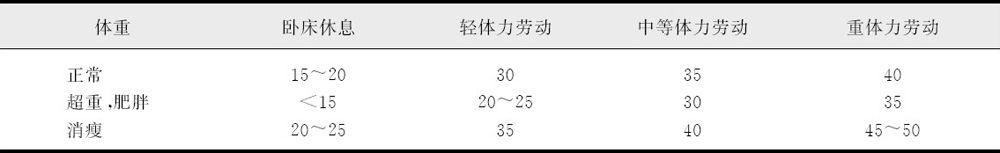
\includegraphics{./images/Image00029.jpg}
\end{table}

注:实测体重占标准体重的±10%为正常范围,10%~20%为超重;>20%为肥胖;-10%~-20%为消瘦。[我国常用的标准体重简易计算:男性:标准体重(kg)=身高-105(cm);女性:标准体重(kg)=身高-105-2.5(cm)]。

标准的减重饮食每天所提供的总能量比维持理想体重所需减少2092~4184kJ(500~1000kcal)。虽然许多病人在6个月内可最多减重10%,但如果不能坚持并随访,易出现体重回升。此外,临床上一般不主张轻易采用极低能量饮食(very
low caloric diet, VLCD)。

(2)平衡的膳食结构

1)碳水化合物:长期以来,糖尿病病人对碳水化合物的摄入一直存在顾虑,认为必须严格限制。近年来实验研究结果提示,在合理控制总能量的基础上适当的碳水化合物摄入量,不会影响病人的血糖值。糖尿病病人每天碳水化合物摄入量应占总能量的55%~65%。目前不推荐采用低碳水化合物饮食(<130g/d)来控制糖尿病病人的超重或肥胖。

一项在1型糖尿病病人中进行的研究显示,餐前胰岛素剂量和餐中碳水化合物总量引起的餐后血糖反应有很大关系。因此,餐前胰岛素的使用剂量应考虑到餐中碳水化合物的含量。对于接受固定剂量胰岛素治疗的病人,每天每餐的碳水化合物量也应一致。

尽管碳水化合物的摄入总量是餐后血糖的主要决定因素,但食物种类、淀粉类型、食物制备方式(如烹饪方法和时间、加热程度或水的用量等)、生熟度和加工程度等对餐后血糖也有影响,因此,碳水化合物的类型对糖尿病病人同样重要。

1984年,Jenkins首次提出了血糖指数(glycemic index,
GI)的概念。通常情况下,血糖指数越低的食物对血糖的升高反应就越小。近年来又有研究指出,餐后血糖水平除了与GI值的高低有关外,还与食物中所含的碳水化合物的含量有密切关系。GI高的食品,如果所含碳水化合物的量很少,尽管其容易转化为血糖,但其对血糖总体水平的影响并不大,因此,GI值仅仅反映出碳水化合物的质,并没有反映出碳水化合物的实际摄入量。如果将摄入碳水化合物的质和量结合起来,就产生了一个新的概念,即血糖负荷(GL)。GL值的大小为食物GI值与其碳水化合物含量两者的乘积:

血糖负荷(GL)=GI×CHO%×100

尽管低GI和低GL食物可能降低餐后血糖,但必须指出,进食速度、食物中脂肪及水溶性纤维含量、胃肠道排空、消化吸收速度和功能都对GI和GL有很大影响,且低GI和GL食物长期的降血糖效应尚待进一步研究证实。

表3-14列出了部分食物的GI值和相应的GL值。

\begin{table}[htbp]
\centering
\caption{中国常见食物GI和GL值}
\label{tab3-14}
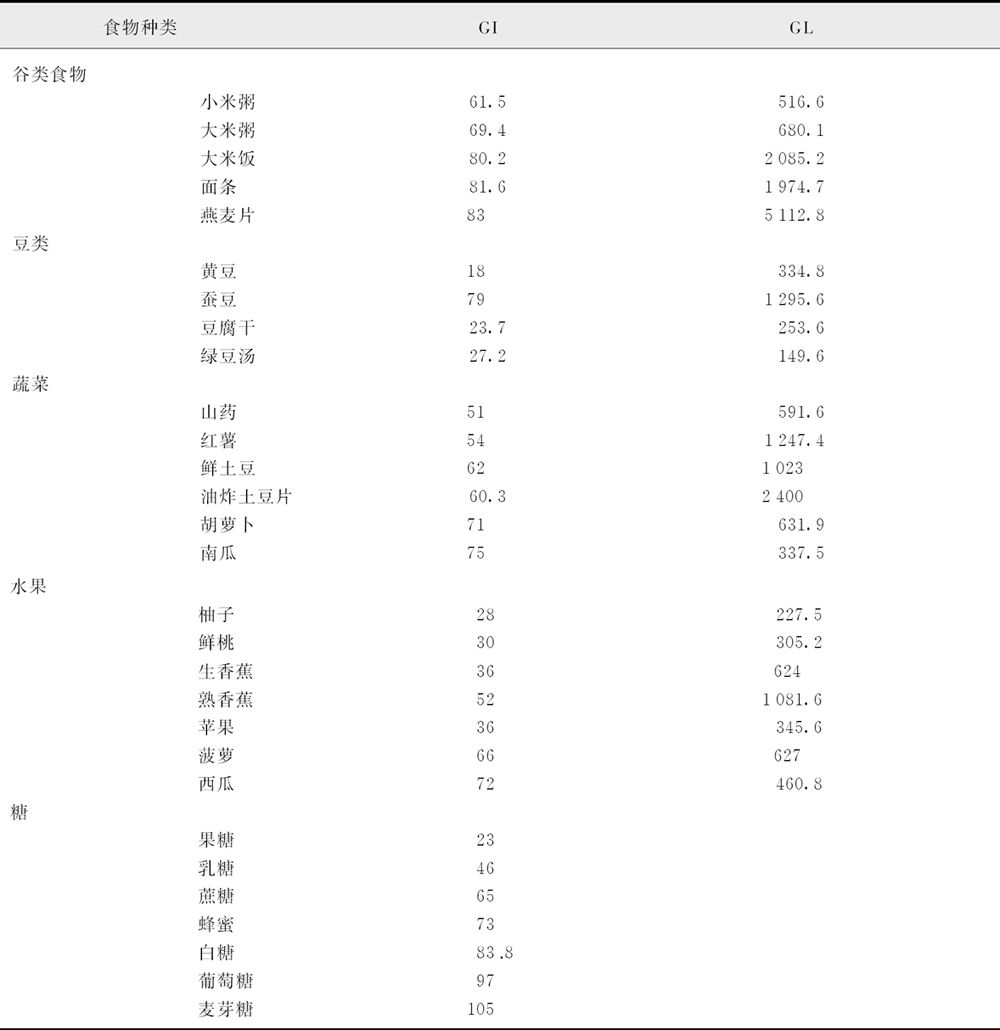
\includegraphics{./images/Image00030.jpg}
\end{table}

鼓励糖尿病病人摄入含膳食纤维丰富的各种食物如豆类、谷类、水果和蔬菜等。因其可以减缓碳水化合物和脂类的吸收从而降低血糖、改善血脂异常、提高机体对胰岛素的敏感性并增加饱腹感。建议糖尿病病人每天摄入膳食纤维30g左右为宜。

研究显示,膳食中的蔗糖虽然甜度很高,但其并不比等能量的淀粉使血糖升得更高,因此,糖尿病病人不必由于担心高血糖加重而刻意限制蔗糖和含蔗糖食物的摄入,只需注意不要因此摄入过多能量。对糖尿病病人,如果在膳食中用果糖代替蔗糖或淀粉,可以产生降低餐后血糖的效应,但因考虑到其可能对血脂有相反作用,所以并不推荐作为增甜剂。糖醇是一种低能量的甜味剂,包括赤藓糖醇、甘露醇、山梨醇、木糖醇、塔格糖等,平均能量含量为8.4kJ/g(2kcal/g)。但并无证据显示其使用可降低血糖、能量摄入或体重。在儿童需注意其摄入可能会引起腹泻。此外,还有一些甜味剂如乙酰氨基磺酸钾、阿斯巴甜、糖精等,不含能量和营养成分,可以在糖尿病人群中使用。

2)蛋白质:糖尿病病人蛋白质代谢异常受胰岛素缺乏和胰岛素抵抗的影响要小于葡萄糖代谢。而单独由碳水化合物引起的血糖反应峰与由碳水化合物和蛋白质共同引起的血糖反应峰是相似的,提示蛋白质不会减慢碳水化合物的吸收。

糖尿病病人每天蛋白质摄入量应为1.0g/kg左右,占总能量的15%~20%,并以优质蛋白质为主。对处于生长发育的儿童或有特殊需要或消耗的人群,蛋白质的比例可适当增高,而对于糖尿病肾病病人,则应特别注意避免过量摄入。此外,目前不建议用高蛋白饮食(>能量摄入的20%)来减轻体重。

3)脂肪:①脂肪摄入量:饮食中如脂肪含量过高,会使血中胆固醇及游离脂肪酸大量增加,导致动脉硬化,降低胰岛素的敏感性,降低葡萄糖的氧化利用率及肝脏、骨骼肌、脂肪等组织的胰岛素受体数目,增加糖异生作用,使血糖升高更为明显。糖尿病病人的每天脂肪需要量通常限制在0.6~1.0g/kg,占总能量的20%~25%。在控制总能量的前提下,低脂高碳水化合物饮食可使体重减轻,同时出现血浆总胆固醇和三酰甘油水平降低、高密度脂蛋白胆固醇(HDL-C)水平升高。如果长期应用,可起到较好的适度减轻体重并改善血脂异常的效果。②不同种类脂肪的比例:ADA建议,糖尿病病人饱和脂肪的摄入应该<总能量摄入的7%。尽管多不饱和脂肪在糖尿病病人中的应用尚未明确,但现有的研究显示,与饱和脂肪相比,多不饱和脂肪仍显示出降低血脂的效应,补充n-3多不饱和脂肪酸(如鱼类)被证明可降低2型糖尿病病人的血浆三酰甘油水平。可是由于多不饱和脂肪酸在体内代谢过程中容易氧化而对机体产生不利影响,故也需限量。与之相比,单不饱和脂肪降低血脂的效应则更为显著,是较为理想的能量来源。为了达到最佳平衡,建议饱和脂肪、多不饱和脂肪与单不饱和脂肪三者的比例控制在0.8∶1∶1.2为宜;而n-3和n-6多不饱和脂肪酸间的比例应为1∶4~6。此外,糖尿病病人对膳食胆固醇比普通人更敏感,所以膳食胆固醇的摄入应<200mg/d。③反式脂肪酸:饮食中反式脂肪酸的主要来源包括用氢化油制成的产品,如烘烤制品(如饼干、面包和其他点心等)、煎炸食品或经氢化起酥的炸鸡等。动物来源的食物如乳制品只提供少量反式脂肪酸。反式脂肪酸升高血浆LDL-C水平的效应类似于饱和脂肪酸。因此,反式脂肪酸的摄入应该限制到尽可能最少。④植物固醇和植物甾醇酯:可以阻断肠道对膳食和胆汁中胆固醇的吸收。有研究报道,每天摄入2g植物固醇/甾醇可降低血浆总胆固醇和LDL-C。

4)微营养素:糖尿病病人应该摄入足够量的维生素和微量元素,特别是对于限制能量摄入的病人,补充多种维生素和微量元素的制剂是有益的,但如果均衡饮食,则无需额外补充,而且需注意如果剂量过大则存在潜在毒性。

由于糖尿病处于氧化应激和慢性炎症的状态,常并发动脉粥样硬化、糖尿病肾病、神经损伤等一系列并发症,所以现在热衷于给糖尿病病人补充抗氧化维生素和微量元素。但目前为止,大剂量膳食抗氧化物如维生素C、维生素E、硒、β胡萝卜素和其他类胡萝卜素在心血管疾病、糖尿病或癌症方面的保护效应并未明确,其长期效应在许多大型研究中并未得到证实,甚至发现可能存在负面效应。因此,在均衡饮食的情况下,并不建议常规补充抗氧化剂。

钙和磷的缺乏或钙、磷代谢紊乱使糖尿病病人更易发生骨质疏松,因此糖尿病病人特别是老年糖尿病病人每天应注意补充。其他某些电解质和微量元素如钾、镁、锌、铬等的缺乏,会加重碳水化合物不耐受。其中锌与胰岛素活性有关,铬可能有利于血糖控制,还有如镁、钒等则可以影响胰岛素的分泌和作用效果。这些微量元素对血糖控制的有益效应虽有报道,但其安全性和长期有效性仍未被大量研究证实,因此补充时需慎重。

(3)糖尿病病人的饮食设计

1)餐次安排和能量分配:糖尿病病人每天至少保证三餐,根据病情必要时加餐。饮食要做到定时、定量、有加餐,但不加量。1型和2型糖尿病不同情况下的餐次能量分配比例见表3-15。

\begin{table}[htbp]
\centering
\caption{不同情况下糖尿病病人每天膳食能量分配比例}
\label{tab3-15}
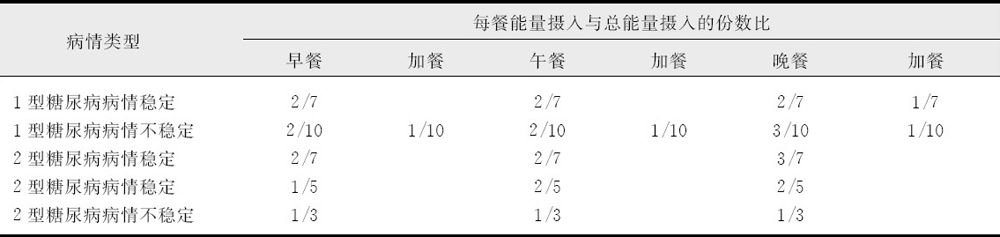
\includegraphics{./images/Image00031.jpg}
\end{table}

2)饮食注意事项:①平衡的膳食结构与正常健康人群相同,糖尿病病人的饮食同样需要均衡摄入不同种类的食物,以满足机体对各种营养素的需求。在限制总能量的条件下,每餐内容粗细搭配、主副食搭配,有利于减缓葡萄糖的吸收,促进胰岛素的释放。②合理选择食物:在碳水化合物中,单、双糖已不再是绝对禁忌,但需在控制的总量范围内;谷类应以粗杂粮代替部分细粮;淀粉类如含糖90%的粉条(干)和含糖10%~20%的马铃薯可以替代部分主食选用。

以蛋白质为主的食物应多选瘦肉,少用肥肉;限量选用鸡、鸭蛋(含蛋白质约13%);多用营养素含量丰富的乳及乳制品。大豆及其豆制品由于所含脂肪多为不饱和脂肪酸,且不含胆固醇,因此可以降低血脂,可部分替代瘦肉。其中大豆含蛋白质约30%,豆腐约含12%。

烹调油由于脂肪含量约100%,故应限量。少用含动物性脂肪的猪油、牛油等,尽量选择植物油如花生油、豆油等。提倡多用含单不饱和脂肪酸的油类如橄榄油和茶油。坚果类如花生仁、核桃仁约含脂肪50%,且属高能量食物,虽有促进胰岛素分泌的作用,但也应限量。

增加新鲜蔬菜尤其是深绿叶菜以及一些含糖量低的叶、茎、瓜果类如菠菜、芹菜、冬瓜、黄瓜和西红柿等的摄入。也可选用菌藻类如海带、紫菜、鲜蘑菇、香菇、木耳等部分代替新鲜蔬菜,具降低血脂的作用。在选择水果时,应注意选血糖指数较低且含丰富维生素与无机盐的品种,如柚子、苹果、猕猴桃等。水果可作为加餐食物,但不宜过量,且应计算在每天总能量内。

在调味料中,钠盐的使用也应特别引起注意。长期高钠饮食会引发高血压,并且加速和加重糖尿病其他心血管并发症的进展。每天盐的摄入量应控制在6g以下甚至更低,做到少吃腌肉、腊肉、色拉酱等含较多盐或钠离子的食物。

病情控制较好时,可少量适度饮酒,但应避免空腹饮酒,以防发生低血糖。而对孕妇和伴有其他疾病如胰腺炎、进展性肾病、严重高三酰甘油血症或酒精依赖的人群应建议戒酒。

由于实际能量消耗通常低于理论值,且存在一定的地域差异,因此饮食管理应该在此原则上进行个体化设计,满足不同病人的实际需要。

(4)饮食计算方法

1)细算法:根据病人一般情况、病情、肝肾功能是否受损、嘌呤代谢是否紊乱和饮食习惯等按食物成分表中各食物的营养素含量计算并设计食谱。细算法一般可分为4个步骤:①确定每天总能量;②确定三大营养素的比例和重量;③确定用餐次数和每餐食物比例;④根据食物成分表和等值食物交换表制定一日食谱。此方法较为准确,但繁琐,不易操作。

2)主食固定法:根据病人病情固定主食用量。一日三餐主食相对固定在250~350g,副食中的瘦肉可食用,每天100~150g(肥胖者50~100g),牛奶250g,蔬菜每天至少约500g。这种计算法主要用于非住院病人,但食物品种单调,易影响生活质量。

3)食物交换份法:食物交换份是将食物按照来源、性质分成数类,同类食物在一定重量内所含的蛋白质、脂肪、碳水化合物和能量相近,不同类食物间所提供的能量也是相同的。由于糖尿病病人的饮食需要根据不同的情况计算各种营养素的能量配比,因此使用食物交换份的方法,可以快速简便地制定食谱,现已广泛得到应用。

食物交换份法将食物分为六大类:主食类、蔬菜类、水果类、鱼肉类、乳类(含豆奶)和油脂类。所有食物均指可食部分,即去皮、籽、核、骨等后的净重。每个食物交换份可产生334.7~376.6kJ(80~90kcal)能量。通常在表中列出各类食物的单位数,可以随意组成食谱。

以下是不同能量需求饮食的交换份(单位)举例(表3-16)以及具体食物举例(表3-17~表3-22)。

\begin{table}[htbp]
\centering
\caption{不同能量饮食内容的交换份(单位)举例}
\label{tab3-16}
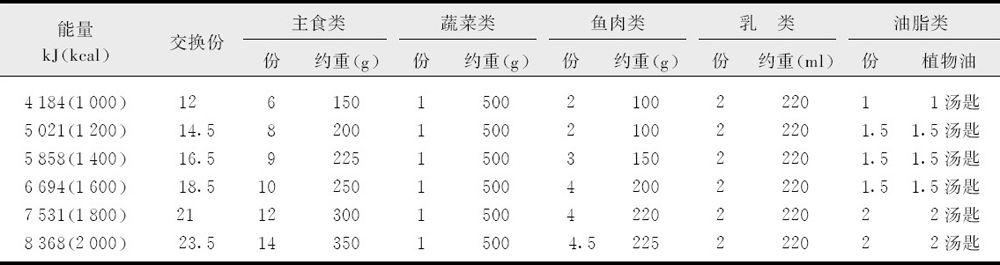
\includegraphics{./images/Image00032.jpg}
\end{table}

\begin{table}[htbp]
\centering
\caption{主食类食物交换份表(谷类、米面类)}
\label{tab3-17}
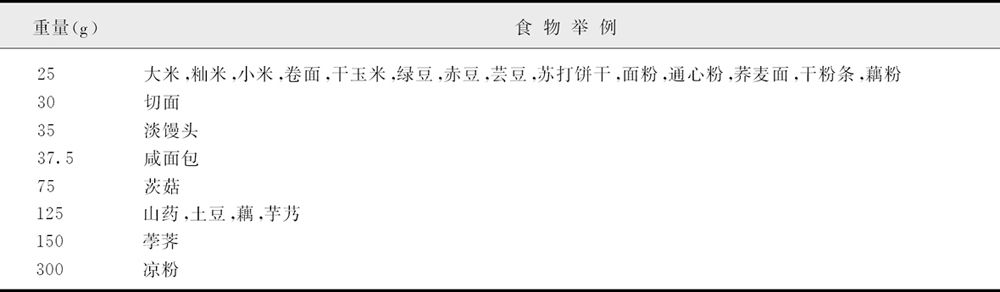
\includegraphics{./images/Image00033.jpg}
\end{table}

注:1个蔬菜类食物交换份可产生334.7kJ(80kcal)能量,其中含有碳水化合物15g、蛋白质5g。

\begin{table}[htbp]
\centering
\caption{蔬菜类食物交换份表}
\label{tab3-18}
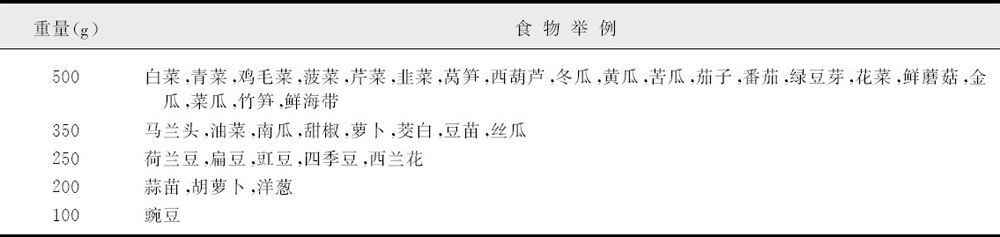
\includegraphics{./images/Image00034.jpg}
\end{table}

\begin{table}[htbp]
\centering
\caption{鱼肉类食物交换份表(含豆制品)}
\label{tab3-19}
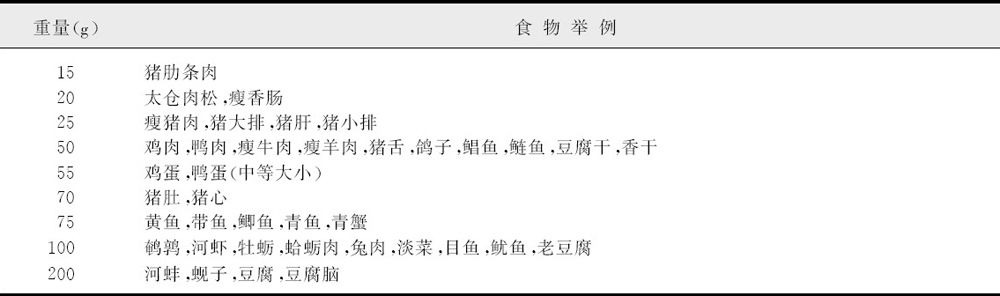
\includegraphics{./images/Image00035.jpg}
\end{table}

注:1个鱼肉类食物交换份可产生334.7kJ(80kcal)能量,其中含有蛋白质9g、脂肪5g。

\begin{table}[htbp]
\centering
\caption{水果类食物交换份表}
\label{tab3-20}
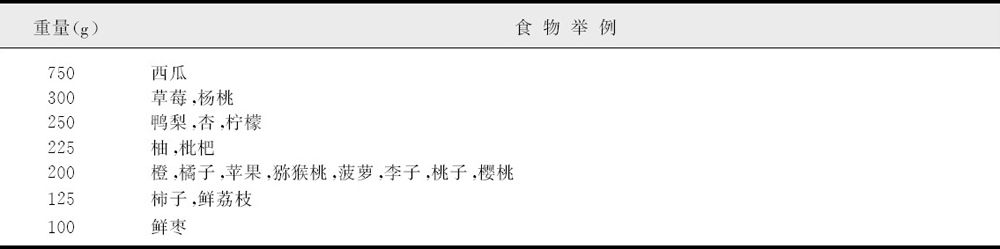
\includegraphics{./images/Image00036.jpg}
\end{table}

注:1个水果类食物交换份可产生376.6kJ(90kcal)能量,其中含有碳水化合物21g、蛋白质1g。

\begin{table}[htbp]
\centering
\caption{乳类食物交换份表(含乳或豆类)}
\label{tab3-21}
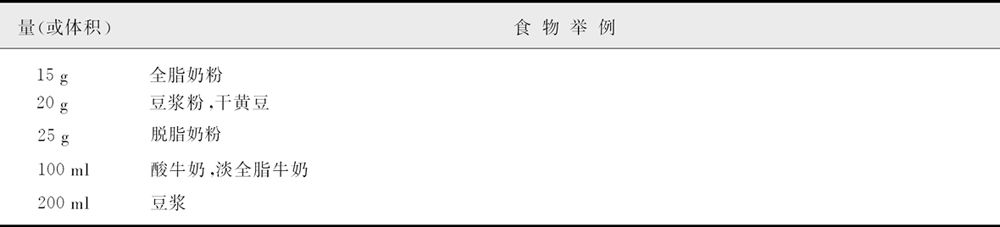
\includegraphics{./images/Image00037.jpg}
\end{table}

注:1个乳类或豆类食物交换份可产生376.6kJ(90kcal)能量,其中含有碳水化合物6g、蛋白质4g、脂肪5g。

\begin{table}[htbp]
\centering
\caption{油脂类食物交换份表}
\label{tab3-22}
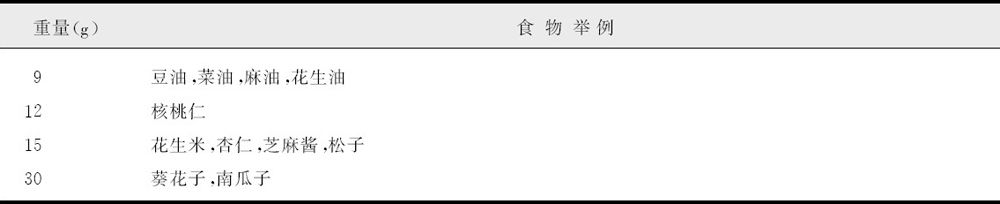
\includegraphics{./images/Image00038.jpg}
\end{table}

注:1个油脂类食物交换份可产生334.7kJ(80kcal)能量,其中含有脂肪9g。

在饮食设计、实施过程中须注意:①至少保证三餐,早、中、晚能量各占25%、40%和35%,对于如注射胰岛素或有低血糖反应者,可加两餐点心,但总能量应保持不变;②水果每天保证0.5~1份,以苹果、柚子等为例,100~200g分2次食用,可作为点心添加;③保证蛋白质的质量和数量,以鱼类和奶类或鸡蛋蛋白为主;④病人应尽快掌握自己每天所吃各类食物的量以及不同能量食品交换的概念和方法。

(四)特殊情况的营养治疗

{1.儿童和青少年糖尿病的营养治疗}
 儿童和青少年大多为1型糖尿病,这一人群的营养目标应该是维持良好的血糖水平的同时保证正常的生长发育,并不出现低血糖反应。这可以通过个体化的膳食计划、灵活的胰岛素治疗方案和自我血糖监测等来达到。

儿童和青春期1型或2型糖尿病病人的具体饮食方案应结合年龄、身高、体重而定。4岁以下者可按209kJ/(kg·d)[50kcal/(kg·d)],4~10岁按188~209kJ/(kg·d)[45~50kcal/(kg·d)],10~15岁按146~167kJ/(kg·d)[35~40kcal/(kg·d)]供给食物。同时,必须考虑儿童的食欲和喜好,且根据不同的目标制定个体化膳食计划。

{2.老年糖尿病病人的营养治疗}
 目前对随着年龄而发生的营养需要改变的研究很有限,针对糖尿病病人的更是缺乏。因此,对老年糖尿病病人的营养治疗建议必须通过已知的正常人群来推断。尽管老年人的能量需要低于中、青年人,但由于各种原因包括疾病导致的可能的摄食减少,使老年糖尿病病人中体重不足比超重更容易发生。在这个年龄组,低体重与较高的发病率和死亡率相关。对住院老年糖尿病病人,由于缺乏食物选择、食物质量差以及不必要的饮食限制,可能会发生营养不良和脱水。因此,建议对住院老年糖尿病病人按常规(非限制)食谱,并固定碳水化合物进食的量和时间以便控制血糖。但对于肥胖的病人,也应适当限制能量摄入。

{3.妊娠、哺乳合并糖尿病的营养治疗}

(1)妊娠糖尿病或糖尿病病人妊娠:孕妇的营养治疗目标是控制血糖的同时,为母亲和胎儿提供足够的能量和各种营养素,并预防酮症酸中毒。因此,妊娠期间并不建议减重,而是应该合理选择食物,使体重在整个孕期适当增加10~12kg;对超重或肥胖的孕妇,应适度限制能量和碳水化合物的摄入。对于妊娠前就患有糖尿病的,应该在准备怀孕前就制定合理的饮食计划。通常情况下,孕妇的能量需要在最初3个月并不增加。但3个月之后,则需适当增加能量和蛋白质的摄入。平衡膳食通常都能提供所需的所有维生素和微量元素,还没有研究结果支持产前额外补充维生素和微量元素制剂,但也需满足特殊的个体需要。

定时、定量进餐和进食点心对于避免由于胎儿持续从母亲体内获取葡萄糖而产生的低血糖是很重要的。晚点心通常可以降低整夜低血糖和空腹酮症的危险性。血糖检测与每天饮食记录为胰岛素治疗和膳食计划的确定提供了有价值的信息。此外,患有糖尿病的妇女应该在怀孕期间避免酒精饮料。

虽然大多数患有妊娠糖尿病的妇女产后会恢复到正常糖耐量,但她们以后再次怀孕时发生妊娠糖尿病或者以后的生活中罹患2型糖尿病的危险性将增加。因此,在分娩后应将生活方式调整的目标定为减轻体重和增加体育运动,降低以后发生糖尿病的危险性。

(2)哺乳:孕前存在糖尿病或患有妊娠糖尿病的妇女建议母乳喂养。母乳喂养可消耗一定能量,从而降低血糖,因此接受胰岛素治疗的妇女通常需要减少胰岛素剂量,并且在哺乳前或哺乳时应适当进食含有碳水化合物的点心。哺乳期头6个月内能量需要比孕期额外增加约837kJ/d(200kcal/d)。

{4.糖尿病急、慢性并发症的营养治疗}

(1)低血糖:饮食摄入量不足、体育运动量增加和药物、胰岛素治疗的调整都可能导致低血糖的发生。由于糖尿病病人的低血糖是体内胰岛素的相对过量,因此,一旦出现血糖<50mg/dl(2.8mmol/L),或即使血糖值未达到此标准,但已远远低于日常水平和出现低血糖症状,都应进行治疗,可立即摄入葡萄糖15~20g,或进食含碳水化合物的食物;稍重者可加馒头或面包25g或水果1个;极少数严重低血糖情况(需要别人帮助和不能自己进食)应紧急注射胰高血糖素。治疗须在10~20分钟内见效,且在60分钟内应再测血糖以观察是否需要补充治疗。发现糖尿病病人低血糖时,如在碳水化合物食物中额外增加蛋白质则对血糖无影响,也不能预防随后的低血糖,而增加脂肪将会延迟升糖反应。对使用胰岛素或口服磺脲类降糖药的病人,必须按时进餐、随身携带糖果饼干、调整运动量后及时调整胰岛素或药物剂量,预防低血糖的发生。

此外,对注射胰岛素和(或)使用胰岛素促分泌剂的病人如果未改变药物剂量或碳水化合物摄入量,运动也可引起低血糖。如果运动前血糖<100mg/dl(5.6mmol/L)应先加餐。仅用饮食治疗或服用二甲双胍、α-葡萄糖苷酶抑制剂及噻唑烷二酮类药物而不用胰岛素者,一般运动前不需加餐。

(2)急重症:糖尿病病人出现急重症或危重病症时可能加重高血糖,并增加1型糖尿病酮症酸中毒的危险性。此外,相关的负调控激素水平的升高可能增加胰岛素的需要。此时,检测血糖和血或尿中的酮体、给予足够量的液体以及摄入碳水化合物都是非常重要的,特别是在血糖水平<100mg/dl(5.6mmol/L)时。在摄入足量碳水化合物的同时应继续进行胰岛素或口服降糖药治疗,保持血糖在目标范围内并预防饥饿性酮症。成人每天摄入150~200g碳水化合物(每3~4小时摄入45~50g)应足以预防饥饿性酮症。

(3)高血压:高血压的营养治疗目标是减轻体重和减少钠的摄入。低脂且富含钾、镁、钙的膳食也能适度降低血压。专家建议钠摄入减少到不超过2400mg/d(100mmol/d)或氯化钠摄入减少到不超过6g/d。此外,增加水果、蔬菜、低脂奶制品摄入、避免饮酒过多、规律的有氧运动等都是降低血压行之有效的措施。ADA
2007年糖尿病诊疗标准中建议糖尿病病人将血压控制在收缩压<130mmHg,舒张压<80mmHg。

(4)血脂异常:1型或2型糖尿病病人通常伴有血脂异常。对大多数1型糖尿病病人来说,有效的胰岛素治疗可以使血脂水平恢复正常并降低血清三酰甘油和LDL-C的水平。对LDL-C升高的成人病人,饱和脂肪酸应该限制在低于总能量摄入的7%,并限制反式脂肪酸和胆固醇的摄入。饱和脂肪酸可用碳水化合物或单不饱和脂肪酸来替代。此外,还可适当增加植物固醇/甾醇和可溶性膳食纤维的摄入。对于肥胖的糖尿病病人,则应进行更严格的限制,并维持适当的体重减轻,增加体育运动。

有些病人即使增加药物治疗,仍存在顽固的高三酰甘油血症,此时,可以选择补充富含n-3脂肪酸的鱼油。但是,鱼油也有升高血LDL-C的可能性,故需严密监测。如果血TG>438mg/dl(11.3mmol/L),发生乳糜微粒血症和胰腺炎的危险性也随之增加,应该限制所有类型的膳食脂肪摄入并使用降脂药物。

(5)糖尿病肾病:许多饮食因素在糖尿病肾病的预防方面起到一定的作用。在有微蛋白尿的1型或2型糖尿病病人,只要轻微减少蛋白质的摄入,就能改善肾小球的滤过率、减少尿白蛋白的排出率。ADA
2007年糖尿病诊疗标准建议,糖尿病肾病早期,即CKD分期早期的病人,蛋白质每天供给量限制在0.8~1.0g/kg;CKD分期为较晚期的病人,蛋白质每天供给量限制在<0.8g/kg可以改善肾功能(尿白蛋白排泄率、肾小球滤过率)。而我国慢性肾脏病蛋白营养治疗共识制定的标准是:从出现显性蛋白尿起即应减少饮食蛋白,推荐蛋白质摄入量0.8g/(kg·d)。从GFR下降起,即应实施低优蛋白质饮食,推荐蛋白质摄入量0.6g/(kg·d)。需注意的是,限制蛋白质的同时不要忽略正常的能量和各种营养素的需要。

{5.糖尿病的肠内、肠外营养支持}
 当糖尿病病人由于疾病不能正常经口饮食或消化吸收能力下降,或因疾病导致蛋白质、脂肪和碳水化合物过度分解并发营养不良时,可给予肠内或肠外营养支持。糖尿病病人的肠内、肠外营养支持原则与非糖尿病病人基本相同,但实际实施时应考虑糖尿病特有的代谢特点和血糖监测的问题。

(1)肠内营养

1)肠内营养的配方:给予糖尿病病人肠内营养时,在满足营养素需求的同时也要达到最佳的血糖和血脂控制,尤其是那些需要长期接受营养支持的病人。在血糖监测和血糖控制稳定的情况下,一些非糖尿病配方也可安全用于糖尿病病人,但要避免过量、过快地提供,应予缓慢持续滴注。

血糖指数的提出已经使缓释淀粉、果糖等血糖指数较低的碳水化合物在糖尿病病人的肠内营养中得到广泛应用。近年来,又有研究提出用单不饱和脂肪酸替代部分复杂糖类,以达到更好的血糖控制效果和代谢状况的改善。在配方中加入膳食纤维,还可减缓胃的排空,降低食物的生糖作用和维持肠道功能。这些方案尤其适用于一些由于神经或机械吞咽困难而需要长期家庭肠内营养的病人。因此,如果病情需要,应该使用这些针对糖尿病的特殊配方肠内营养制剂,临床研究结果表明,它不但可以改善血糖水平、减少降糖药物使用剂量,而且可以降低感染的发生率。

2)肠内营养的实施:①输注方式:为了更好地控制血糖、减少胃肠道反应,推荐使用输液泵维持的连续滴注方式给予糖尿病病人肠内营养支持;②胰岛素的使用:疾病或创伤所致的应激反应可能引起胰岛素抵抗,此时,非胰岛素依赖型的糖尿病病人可能也需给予胰岛素,而胰岛素依赖型的糖尿病病人则可能需要量比平时更多。

(2)肠外营养

1)肠外营养的配方:将糖和脂肪一同作为能量来源可减轻糖负荷和血糖反应。糖尿病病人葡萄糖的推荐量与非糖尿病病人相似,为4~5g/(kg·d),但需注意输注速率;通常情况下,脂肪的供给量也与非糖尿病病人相似,但病情加剧时应适当减少。

2)肠外营养中胰岛素的使用:肠外营养应用于糖尿病病人时需根据其中葡萄糖的含量和血糖变化在全营养混合液(total
nutrient admixture,
TNA)输注袋中额外添加胰岛素,并补充钾和磷,且应维持稳定的输注速度,不宜过快。尽管胰岛素加入输注袋内会被塑料吸附而丢失约30%,但优点是当输注停止时胰岛素也随即停止输入。有研究者建议,将所需胰岛素总剂量的2/3加入TNA中,余下剂量通过其他方式给予,以便根据血糖水平及时调整胰岛素用量,对于围手术期和糖代谢不稳定的病人尤有意义。

3)营养支持期间的血糖监测:除了体重、体液平衡、血电解质等,血糖是糖尿病病人营养支持过程中最重要的监测项目。血糖平稳病人的血糖水平突然发生变化可能是感染的一个早期信号。刚开始营养治疗时可每6小时测定1次血糖,稳定后再减少监测次数。随时注意有无非酮症性高渗性脱水和昏迷等危急情况的发生,并及时发现并处理。

需特别注意的是,当TNA输入突然终止时,也可发生低血糖反应,这是由于胰岛素在循环中的半衰期仅3~4分钟,其作用在输入停止后会立即失效。因此,应按之前营养液的输注速率给予10%的葡萄糖2~3小时以预防低血糖的发生。

\hypertarget{text00004.htmlux5cux23mllj25}{%
\section{ 营养与高尿酸血症及痛风}\label{text00004.htmlux5cux23mllj25}}

随着社会经济的发展以及人民生活水平的提高、生活方式和膳食结构的改变,痛风的患病率不断上升,使素有“富贵病”之称的痛风成为了一种常见病。

痛风(gout)是嘌呤代谢紊乱和(或)尿酸排泄减少,血尿酸增高引起组织损伤的一组异质性疾病。其临床特点为高尿酸血症、反复发作的特征性急性关节炎、痛风石形成、痛风性肾实质损害,严重者呈关节强直或畸形及功能障碍,常伴有尿酸性尿路结石。以上临床表现可以不同的组合方式出现,但仅有高尿酸血症,即使合并尿酸性尿路结石也不称之为痛风。痛风是指高尿酸血症同时伴有反应性关节炎或痛风石等病变。

\hypertarget{text00004.htmlux5cux23mllj26}{%
\subsection{发病机制及诊断}\label{text00004.htmlux5cux23mllj26}}

(一)流行病学

痛风过去在欧美国家较常见,而在亚洲较为少见。20世纪80年代,美国报道痛风的患病率为0.275%,到1993年Star报道美国的痛风患病率已接近1%,1995年Harris报道英国的痛风发病率也已达1%。欧美地区高尿酸血症的患病率为2%~18%。而在中国,1980年方圻等对北京、上海、广州、杭州20岁以上的成年人进行血尿酸调查,发现高尿酸血症的患病率为1.4%,未发现一例痛风病人。1990~1992年,陈顺乐等COPCORD调查痛风患病率为0.2%。1998年,杜惠、陈顺乐等报道上海黄浦区痛风患病率调查结果为0.34%,高尿酸血症患病率为10.1%。1995年杨岫岩等调查国内21家城市医院1979~1993年的住院病人发现,15年间痛风的住院构成比有直线上升趋势,尤其是南方沿海城市升高更为明显。1998年Chou等报道台湾中部土著居民痛风患病率为11.7%,高尿酸血症的患病率高达41.4%。2005年陈伟等对北京地区部分人群(参加医院年度体检的国家机关和事业单位人群)进行横断面调查,发现高尿酸血症发病率为10.9%。2006年苗志敏等调查2004年山东沿海地区20岁以上居民高尿酸血症和痛风患病率,发现高尿酸血症的患病率为13.19%,痛风的患病率为1.14%。2007年徐厚兰等调查绍兴某医院健康体检人群高尿酸血症患病率为11.89%。2007年胡守岳等报道宁波某区居民2005年健康体检人群高尿酸血症患病率为16.42%。由此可见,无论是欧美,还是亚洲等国家,高尿酸血症与痛风的患病率都有逐年上升趋势。高尿酸血症与痛风是慢性代谢性疾病之一,因此其防治应与防治糖尿病、高血压、心脑血管疾病一样重要。

虽然高尿酸血症多发生于成年人,但随着儿童肥胖率的增加,作为其代谢并发症之一的高尿酸血症也出现在儿童及青少年中。关于青少年肥胖并发高尿酸血症的调查不多。2006年朱建芳、梁黎等对浙江大学医学院附属儿童医院2003~2005年因肥胖住院的青少年进行调查,发现高尿酸血症在中、重度肥胖青少年中的发病率分别为19.18%和24.32%。

与其他慢性代谢性疾病一样,高尿酸血症发病呈低龄化趋势,儿童与青少年的健康关系到其成年时的健康,关系到祖国的未来,因此痛风的防治刻不容缓,且良好的健康生活方式应从小培养、干预。

(二)发病机制

尿酸是嘌呤代谢的最终产物。人体内嘌呤的合成主要在肝内进行。嘌呤的合成和代谢途径及其反馈调节机制详见图\ref{fig3-2}。

\begin{figure}[!htbp]
 \centering
 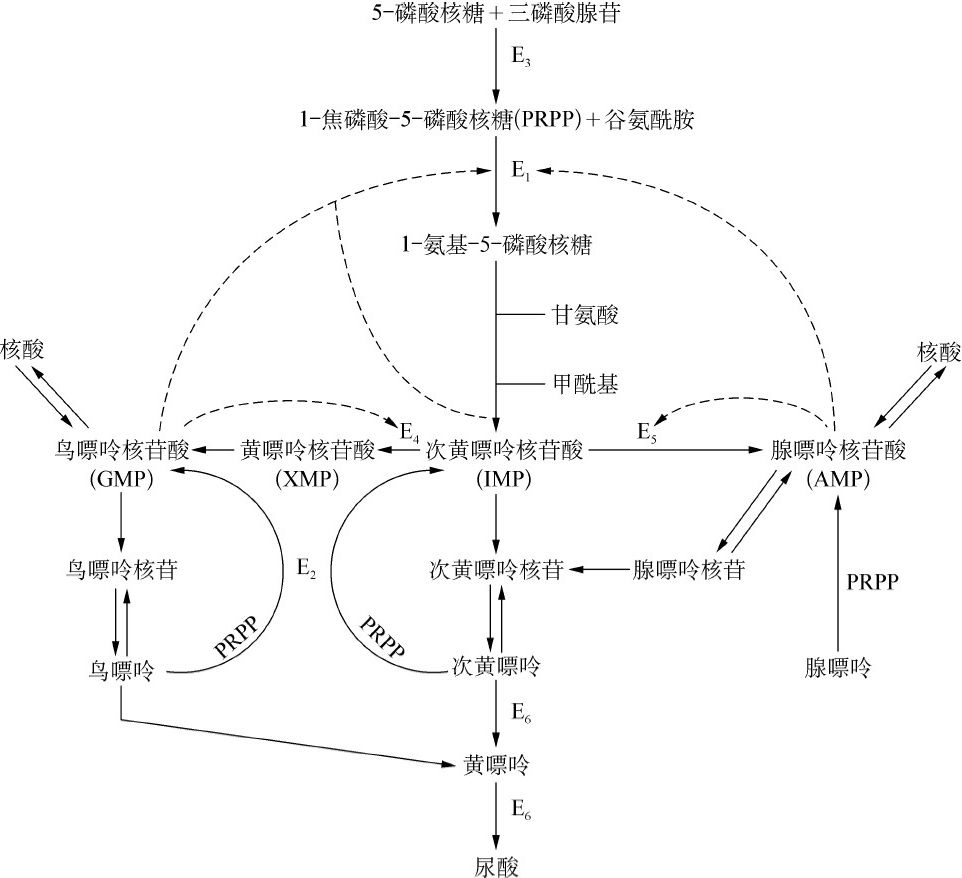
\includegraphics{./images/Image00039.jpg}
 \captionsetup{justification=centering}
 \caption{嘌呤合成和代谢途径及其反馈调节机制}
 \label{fig3-2}
  \end{figure} 

E\textsubscript{1} :磷酸核糖焦磷酸酰胺转移酶;E\textsubscript{2}
:次黄嘌呤-鸟嘌呤磷酸核糖转移酶;E\textsubscript{3}
:PRPP合成酶;E\textsubscript{4}
:次黄嘌呤核苷-5′-磷酸脱氢酶;E\textsubscript{5}
:腺苷酸代琥珀酸合成酶;E\textsubscript{6} :黄嘌呤氧化酶→表示负反馈控制

人体内尿酸有两个来源:①外源性:约占体内总尿酸的20%,从富含嘌呤或核蛋白食物而来;②内源性:约占体内总尿酸的80%,由体内氨基酸、核苷酸及其他小分子化合物合成及核酸代谢而来。正常人体内尿酸池平均为1200mg,每天产生750mg,其中1/3的尿酸从肠道排出,肠道细菌有尿酸酶,使尿酸转变成尿囊素,最后分解为二氧化碳和氨随粪便一起排出,其余2/3尿酸由肾脏排出。尿酸排泄主要依靠肾小管再分泌。分泌部分代表总尿酸的80%。血尿酸增高的主要环节是肾小管分泌下降,也包括重吸收增加。

尿酸在细胞外液的浓度取决于尿酸生成和肾脏排出之间的平衡关系,嘌呤合成代谢增高和(或)尿酸排泄减少是体内血清尿酸值增高的重要机制。在原发性高尿酸血症和痛风病人中90%是由于尿酸排泄减少,尿酸生成增多所致者仅占少数。高尿酸血症病人中只有10%~20%发生痛风。其发生是由于尿酸在体内处于过饱和状态。

(三)病因及分类

高尿酸血症的发病受到许多因素的影响。Nakajima认为大多数高尿酸血症病人处于多种危险因素共同作用的环境中,首次提出高尿酸血症是典型的生活方式疾病,它与性别、年龄、饮食以及遗传等诸多因素密切相关。

{1.遗传因素}
 痛风与遗传有一定的关系。美国的非洲裔人群患病率高于高加索人群;新西兰的毛里人(Maori)痛风患病率高于当地其他人群;我国台湾中部土著居民的痛风患病率高于其他人群,均提示痛风与遗传有关。原发性痛风病人中,有痛风阳性家族史者占10%~25%,其近亲中发现有15%~25%患高尿酸血症。

痛风和高尿酸血症属于复杂的多基因遗传病。研究发现,原发性痛风可能是一种伴性遗传的常染色体显性遗传,但外显性不完全,其可能是在多基因控制的背景下,有一个常染色体显性基因在发挥主要作用,性别对这个基因作用有明显影响。

{2.环境因素}
 环境因素对于本病的发生很重要。例如:高嘌呤饮食、过度饮酒及饥饿等状态;肥胖、高血压、肾功能不全等疾病及使用利尿剂、小剂量水杨酸和滥用泻药等均可造成高尿酸血症。

近年来认为有些环境因素导致痛风和高尿酸血症是由于ATP加速分解导致其代谢产物次黄嘌呤、黄嘌呤及尿酸明显增加所致。剧烈运动、酗酒、缺氧、外科手术、化疗及放疗等均可使ATP分解加速、合成减少,从而引起临床高尿酸血症的发生。

(四)临床表现

原发性痛风大部分发病在40岁以上,以中、老年多见,其中男性约占95%,女性多数在更年期后发病。高尿酸血症大多发生在男性,可能与雌激素促进尿酸排泄及男性中某些酶基因突变致活性改变有关。

有研究表明,原发性痛风患病率男女性之比约为20∶1,高尿酸血症患病率男女性之比约为2∶1。高发年龄组男性为50~59岁,女性为50岁以后。高尿酸血症和痛风的患病率随年龄增加而增高。

典型痛风的自然病程经历4个阶段,即无症状性高尿酸血症、急性痛风性关节炎、间歇期、痛风石与慢性痛风性关节炎。

{1.无症状性高尿酸血症}
 无症状性高尿酸血症是指血清尿酸升高,但无关节炎发作,因此与有症状的痛风之间是有区别的,不是痛风的同义词。血液中尿酸钠的饱和度约为404μmol/L(68mg/L)。男性血尿酸>416μmol/L(70mg/L),女性血尿酸>357μmol/L(60mg/L)即称为高尿酸血症。血清尿酸浓度越高,发展成为痛风的趋势就越大,当痛风性关节炎第一次发作后,无症状性高尿酸血症即宣告结束。从血尿酸增高至症状出现,时间可长达数年至数十年,其转变的确切机制未明,有些病人可终生不出现症状。

{2.急性痛风性关节炎}
 急性痛风性关节炎是痛风最常见的首发症状。四季均可发病,但以春、秋季节多发。受寒、劳累、过度饮酒、饥饿、高嘌呤饮食及感染、创伤、手术等为常见的诱因。典型症状是突然发病,通常第一次发作是在夜间,多起始于凌晨1~2点,因疼痛而惊醒,初起85%~90%为单关节受累,受累关节以第一跖趾为多见。在几小时之内,受累关节变得暗红、肿胀、发热、疼痛剧烈,活动受限。疼痛高峰在24~48小时,初次发作可呈自限性,病程持续时间在数小时至数日不等。发作缓解后,关节功能恢复,受累关节部位可出现脱屑和瘙痒,为本病特有的症候,但非经常出现。如急性发作治疗不当,关节炎可迁延不愈或转移至其他关节。

{3.间歇期}
 两次发作之间的一段静止期称为间歇期。大多数病人一生之中反复发作多次,个别病人一生仅发作1次。多数病人第二次发作在6个月至2年之间,少数病人间隔时间可长达5~10年。一般情况下,未经有效治疗的病人,发作频率渐频,间歇期缩短,症状加剧。随着病程发展,常累及多个关节,发作持续时间也变长。但有些病人第一次发作后没有缓解期,直接进入亚急性期和慢性期。

{4.痛风石与慢性痛风性关节炎}
 由于尿酸沉积于结缔组织,逐渐形成痛风石。痛风石是痛风特征性损害。Hench报道痛风石形成的时间在痛风首次发病后3~42年不等,平均为11.6年。其发生率与高尿酸血症持续时间及严重程度呈正相关。痛风石为不规则黄白色赘生物,其核心是尿酸钠结晶。痛风石出现的最典型部位在耳轮,其他常见部位为第一大足趾、指、腕、膝、肘等,甚至可累及心脏。关节附近的痛风石,表皮磨损易溃破和形成瘘管,可排出白色尿酸钠结晶。在未用药物治疗的病人中,约有半数病人出现痛风石。

痛风病人经过10~20年演变,累及上下肢各关节。由于痛风石不断增大、增多,软骨及关节周围结缔组织尿酸盐沉着,纤维增生,骨质破坏,最终导致关节强直、畸形,可出现假性类风湿关节炎样关节,使功能完全丧失。

{5.肾脏病变}
 痛风导致肾脏病变最主要是由于血尿酸增高,尿酸盐在肾脏内沉积所致。20%~40%的痛风病人有慢性肾脏病变,这与痛风病程的长短及治疗控制的好坏密切相关。病人早期可有腰痛、水肿、轻度蛋白尿、镜下血尿、高血压等表现。病程发展至晚期,可出现肾功能不全,病人可因尿毒症而死亡。如早期诊断并治疗,肾脏病变可减轻或停止发展,这点与其他不可逆的肾病有区别。

{6.肾结石}
 尿酸性肾结石是由于尿酸结晶沉积在肾和尿路,形成大小不一的结石,小如细沙粒状,大如黄豆,或呈鹿角形样巨大结石。在痛风病人中,尿中尿酸排泄正常者约20%发生肾结石,尿中尿酸排泄增高者约40%发生肾结石。男性较女性多见。细沙粒状结石常无症状,常随尿排出而不为人察觉。较大的结石造成输尿管梗阻时,可引起肾绞痛和血尿。巨大结石可导致肾盂肾盏变形、肾盂积水。有的病例可并发尿路感染。

(五)诊断

典型的痛风容易诊断。多为40岁以上男性,有肥胖、嗜酒等诱发因素,部分有家族史。有典型的关节炎发作表现(关节炎发作多见于下肢远端足趾关节,半夜发作,剧痛,白天缓解)。秋水仙碱治疗有效。此外还有高尿酸血症和高尿酸尿症。慢性痛风的诊断依据是病史和痛风石。

可采用下述诊断标准:

(1)血尿酸男性>416μmol/L(70mg/L),女性>357μmol/L(60mg/L)。

(2)有痛风石。

(3)关节液内找到尿酸钠结晶或组织内有尿酸钠沉积。

(4)有2次以上发作。

(5)有典型的关节炎发作(突然发病,夜剧昼缓,局限于下肢远端)。

(6)用秋水仙碱治疗,48小时内缓解。

如上述标准中有两项符合,即可诊断为痛风。

\hypertarget{text00004.htmlux5cux23mllj27}{%
\subsection{高尿酸血症与痛风的预防和治疗}\label{text00004.htmlux5cux23mllj27}}

(一)预防和治疗

痛风防治需达到以下目的:①尽快终止急性症状,预防急性关节炎复发;②纠正高尿酸血症;③减少并发症的产生或逆转并发症。

{1.无症状性高尿酸血症的处理}
 目前意见不一。一般认为无症状性高尿酸血症几乎不需要治疗,但需避免肥胖、高能量及高嘌呤饮食以及疲劳、酗酒、饥饿、创伤、精神紧张等诱发因素。如血尿酸明显增高,仍应考虑药物治疗。

{2.急性期的处理}
 绝对卧床休息,抬高患肢,以促进局部的血液循环,避免受累关节负重。一般应休息至关节疼痛缓解72小时后才可开始活动。局部冷敷有助于缓解疼痛,而热敷则可能加剧炎症。一旦诊断明确,应尽早予以药物治疗。治疗越早,疗效越好。开始用药的时机远比具体使用哪一类药物更重要。常用药物有以下几种。

(1)秋水仙碱:过去普遍将秋水仙碱作为痛风急性发作的首选药。首次剂量1mg,以后每2~3小时口服0.5mg,直至关节症状好转或出现恶心、呕吐、腹泻等胃肠道反应不能耐受时予停药。第一天的最大剂量6~8mg,第2~3天每天2mg,之后每天1mg维持15天。

然而,事实上秋水仙碱并不总是有特效,原因可能与其用药时机有关。急性发作24小时内用药效果较好,2/3病人于用药后6~12小时症状可减轻,24~48小时内症状可缓解。如果发作已持续数天再用药则效果不佳。而且50%~80%的病人在出现疗效前即已出现胃肠道不良反应。因此近年来更多地使用非甾体抗炎药。

(2)非类固醇抗炎药(NSAID):包括吲哚美辛(indomethacin,消炎痛)、布洛芬、保泰松等。此类药物较秋水仙碱温和,其中以吲哚美辛最为常用。其开始剂量50~75mg,以后每隔6小时25~50mg,第一天最大剂量150mg,第3~4天改为每天75~100mg。NSAID能在24小时内明显缓解急性痛风性关节炎的症状,因此可作为一线药物使用。不良反应主要为急性胃黏膜病变、肾功能损害。但因只是在急性发作时短时间使用,所以影响不大。对于害怕出现胃肠道反应者,也可选择使用其栓剂。

(3)糖皮质激素:能迅速缓解痛风急性发作,但停药后往往出现“反跳现象”(复发),因此只在秋水仙碱、非甾体类抗炎药治疗无效或有禁忌证时采用。泼尼松(强的松)口服剂量为10mg,每天3~4次。急性发作控制后口服激素逐渐减量或同时加用小剂量秋水仙碱(0.6mg/次,每天2次)以预防“反跳”。对1~2个大关节发作者可考虑关节腔内给药。

对于反复发作的痛风病人,除了要避免各种诱发因素外,还应使用小剂量秋水仙碱或NSAID维持治疗以预防再次急性发作。

{3.发作间歇期及慢性期的处理}
 主要是使用促使尿酸排泄或抑制尿酸生成的药物,以控制高尿酸血症,使血尿酸维持在正常范围,防止复发。血尿酸突然波动可能会诱发急性痛风性关节炎。为预防降尿酸药可能引起的关节炎急性发作,应在开始加用的前6个月同时予以小剂量秋水仙碱,即0.6mg/次,每天2次。肾功能不全病人应减小剂量,70岁以上老年病人上述维持剂量应减半。降尿酸治疗是连续和长期的,甚至是终生的。

(1)排尿酸药:主要通过抑制近端肾小管对尿酸的重吸收而促进尿酸排泄。适用于血尿酸升高、肾功能正常或轻度受损,肾尿酸排泄减少(24小时尿酸排出量<600mg)的病人。治疗时一般从小剂量开始,逐步加大剂量(每3~4周加1次),使血尿酸缓慢、平稳降至目标值,然后以最小有效剂量维持治疗。服药期间应鼓励病人大量饮水并碱化尿液,特别是要防止夜间尿液浓缩和酸化。碱化尿液可提高尿酸溶解度,促进尿酸盐结石溶解。常用药物如下。

1)丙磺舒(probenecid):开始剂量为250mg,每天2次,以后逐渐增至500mg,每天3次。最大剂量每天不宜超过2000mg。不良反应为胃肠道刺激、过敏、皮疹、骨髓毒性等。

2)磺吡酮(苯磺唑酮,sulfinpyrazone):为保泰松的衍生物,其排尿酸作用较丙磺舒强,不良反应则较丙磺舒少,病人较易耐受,但对骨髓毒性的发生率较高。开始剂量为50mg,每天2次,以后逐渐增至100mg,每天3次,每天最大剂量不宜超过600mg。与丙磺舒一起使用有协同作用。

3)苯溴马龙(benzbromarone):作用机制同磺吡酮,但作用更强,不良反应较前两者低。开始剂量为25mg,每天1次,以后可逐渐增至每天100mg。

(2)抑制尿酸合成药:其作用机制为通过抑制黄嘌呤氧化酶而使尿酸生成减少。适用于尿酸生成过多或不适宜使用排尿酸药的病人。目前应用的只有别嘌呤醇(allopurinol),剂量为每次100mg,每天2~4次,最大剂量可用至每天600mg。不良反应有胃肠道不适、皮疹、发热、关节痛,骨髓抑制少见。多发生于肾功能不全病人,故病人如有肾功能不全,别嘌呤醇剂量宜减半。

(二)营养治疗

过去一直认为高尿酸血症对人体的影响主要是尿酸盐结晶沉积在关节和肾脏而引起相应的病变。近年许多研究表明,高尿酸血症与代谢综合征(metabolic
syndrome,
MS)结伴出现,并已成为代谢综合征的一部分。MS是伴有胰岛素抵抗的一组疾病的集合,包括中心性肥胖、糖耐量异常、高血压、脂质代谢紊乱以及微量蛋白尿等代谢异常。临床上一半以上的原发性痛风病人伴发上述疾病的一种或数种。

研究表明,高尿酸血症与肥胖、高血压、高密度脂蛋白水平低、高三酰甘油血症、高胆固醇血症及伴胰岛素抵抗的高胰岛素血症密切相关。肥胖影响血尿酸代谢,其机制可能与内分泌紊乱(雄激素和ACTH水平降低)或酮体生成过多抑制尿酸排泄有关。高血压病人存在大血管和微血管病变,局部组织缺氧使血乳酸水平增高,与尿酸竞争排出体外导致肾脏清除尿酸能力减退;而血尿酸水平增高,又可增强肾小管钠的重吸收功能,从而导致高血压。高尿酸血症与上述疾病相互联系和影响可能与胰岛素抵抗有关。在胰岛素抵抗状态下,糖酵解过程中的中间产物向5-磷酸核糖及磷酸核糖焦磷酸转移,导致血尿酸生成增多,同时也使3-磷酸甘油积聚,使血三酰甘油浓度增加。伴有高三酰甘油血症的胰岛素抵抗是高尿酸血症的一个特征。过高的血尿酸浓度可直接损伤胰腺β细胞,进而诱发糖尿病。因此控制体重、合理膳食、养成良好的生活习惯、加强对痛风病人的健康教育对于预防和治疗痛风及其相关疾病都是很重要的。对痛风的营养治疗具体措施如下。

{1.合理膳食结构}

(1)限制总能量的摄入以保持适宜体重:研究表明高尿酸血症与体重、体质指数(BMI)、腰臀比(WHR)等呈正相关。体重与代谢性疾病的关系不仅与肥胖的程度有关,而且与肥胖的类型关系更为密切。中心性肥胖病人更易患高尿酸血症与痛风。2007年江新泉等对体检者检查资料进行研究发现肥胖组血尿酸水平显著高于非肥胖组。

对于肥胖病人,应限制每天摄入的总能量,每天给予每千克理想体重83.7~104.6kJ(20~25kcal)以减轻体重。体重减轻应循序渐进,如实际摄入量与此相差较大,则可每阶段减少2092kJ(500kcal),逐步达到正常体重;如实际摄入量与此相差不大,则可一步到位。体重减轻切忌过快,以免机体产生大量酮体与尿酸互相竞争排出,造成血尿酸升高,促使痛风急性发作。美国麻省Framingham的研究资料表明,男子的相对体重减少10%,可使血尿酸下降19.6mmol/L。

近年来儿童肥胖发生率呈逐年上升趋势,儿童肥胖可持续发展为成人肥胖。肥胖是代谢性疾病的重要致病因素。因此,预防肥胖应从小做起,家长应以身作则,培养儿童良好的饮食习惯。2006年尤国文等报道关于肥胖儿童血清尿酸水平的研究发现肥胖儿童的血清尿酸显著高于对照组。

(2)适量摄入碳水化合物:碳水化合物作为能量的主要来源,可防止组织分解及产生酮体,并有增加尿酸排泄的倾向。在总能量限制的前提下,碳水化合物一般占总能量的50%~60%。果糖能增加腺嘌呤核苷酸的分解,加速尿酸的合成,因此尽量减少果糖的摄入。蜂蜜含果糖较高,不宜食用。蔗糖和甜菜糖分解后会产生果糖,亦应少食。

有研究表明,提高机体对胰岛素的敏感性有利于尿酸排出。Dessein等建议应适当限制碳水化合物的摄入,按比例增加蛋白质及不饱和脂肪酸的摄入,提高机体对胰岛素的敏感性,从而促进血尿酸的排出。

(3)低脂饮食:脂肪占总能量的30%以下,其中饱和、单不饱和、多不饱和脂肪酸比例约为0.8∶1.2∶1,每天脂肪摄入总量控制在50g以内。清淡的饮食一方面可以减少能量的摄入,有助于减轻体重;另一方面也可以减少脂肪分解产生的酮体对肾脏排泄尿酸的抑制作用。

(4)适量蛋白质:蛋白质的摄入应占能量的10%~15%,或每天每千克理想体重0.8~1.0g。可选择牛奶、鸡蛋等优质蛋白及植物蛋白。牛奶、鸡蛋无细胞结构,不含核蛋白。酸奶中含乳酸较多,乳酸可与尿酸竞争从肾脏排出,对痛风病人不利,故不宜饮用。

(5)低盐饮食:食盐中的钠有促使尿酸沉淀的作用。痛风病人多伴有高血压,宜采用低盐饮食。

(6)适当补充维生素与微量元素:由于长期忌嘌呤或低嘌呤饮食,限制了肉类、内脏及豆制品的摄入,因此要适当补充各种维生素和微量元素。B族维生素及维生素C的补充很重要,因为它们可促进组织中尿酸盐的溶解。

{2.避免高嘌呤饮食}
 尽管高尿酸血症的发生主要是由于内源性代谢紊乱所致,但高嘌呤饮食可使血尿酸浓度升高,甚至达到痛风病人的水平,常可造成急性痛风性关节炎的发作。一般人日常膳食嘌呤摄入量为600~1000mg。在急性期,嘌呤摄入量应控制在每天150mg以内,以免增加外源性嘌呤的摄入,宜选择嘌呤含量低的食物。缓解期要求正常平衡膳食,可适量增选嘌呤含量中等的食物。无论在急性期还是缓解期,均应避免嘌呤含量高的食物。

现根据嘌呤含量的高低将食物分类,详见表3-23、表3-24及表3-25。

\begin{table}[htbp]
\centering
\caption{嘌呤含量高的食物(每100g食物嘌呤含量150~1000mg)}
\label{tab3-23}
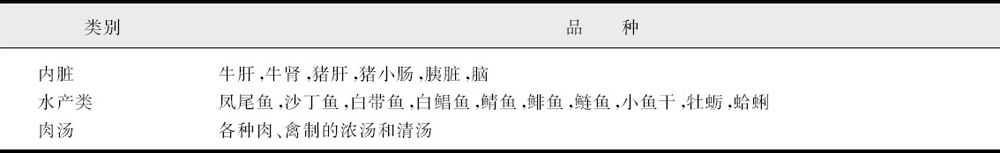
\includegraphics{./images/Image00040.jpg}
\end{table}

\begin{table}[htbp]
\centering
\caption{嘌呤含量中等的食物(每100g食物嘌呤含量50~150mg)}
\label{tab3-24}
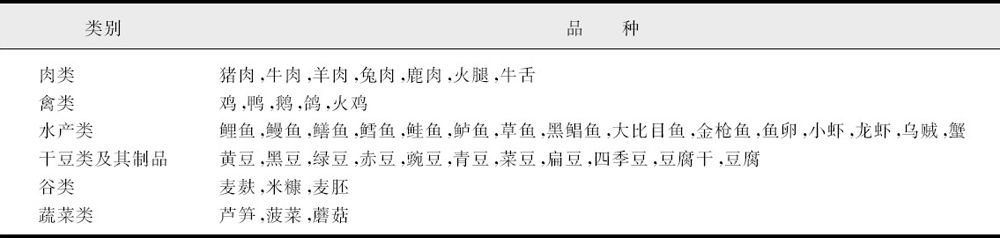
\includegraphics{./images/Image00041.jpg}
\end{table}

\begin{table}[htbp]
\centering
\caption{嘌呤含量很少的食物(每100g食物嘌呤含量<50mg)}
\label{tab3-25}
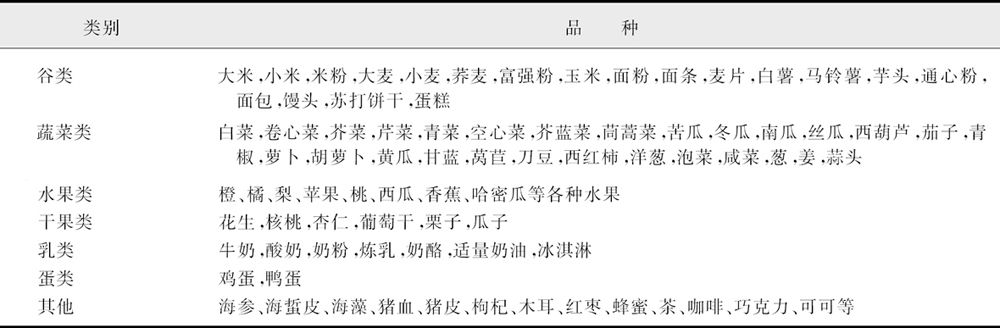
\includegraphics{./images/Image00042.jpg}
\end{table}

{3.多食新鲜蔬菜、水果为主的碱性食物}
 尿液的pH值与尿酸盐的溶解度有关。pH值在5.0时,每分钟只能溶解尿酸盐60mg,而pH值在6.6时,几乎所有的尿酸盐均呈游离状态。急性痛风性关节炎病人尿pH值最好保持在6.5~6.8,这样不仅可以防止尿酸盐结晶,而且可以使已形成的尿酸盐结石溶解。

增加碱性食物的摄入可升高尿液的pH值,有利于尿酸盐的溶解。碱性食物是指含有较多的钾、钠、钙、镁等元素的食物,可在体内氧化生成碱性离子。常见的有各类蔬菜、水果、紫菜、海带、海藻及马铃薯、甘薯、奶类等。西瓜和冬瓜不但属于碱性食物,且有利尿作用,对痛风治疗有利;而菠菜、蘑菇、芦笋含嘌呤较多,少食为佳。

{4.水分摄入要充分}
 每天摄入充足的水分有利于体内尿酸的排出。痛风病人只要肾功能正常,每天饮水应达到2000ml以上,约8~10杯水,伴肾结石者最好达到3000ml。睡前或夜间亦应补充水分以防止尿液浓缩。水分摄入应以白开水、淡茶水、矿泉水及新鲜果汁等为主。

{5.戒酒}
 酒精不仅增加尿酸合成,而且使血乳酸浓度升高,抑制肾小管分泌尿酸,造成肾脏排泄尿酸减少。台湾的营养与健康调查显示,痛风患病率较高的土著人饮酒量明显高于一般人群。因此,痛风病人应戒酒。

近年来研究发现,痛风与饮酒的相关性不仅与酒量有关,而且与酒的类型也有关。啤酒与痛风的相关性最强,烈酒次之,中等量以下的红酒不增加痛风的危险性。啤酒中含有大量嘌呤,且主要是鸟嘌呤核苷。鸟嘌呤核苷比其他核苷、核苷酸或碱基更容易吸收。另有研究发现,啤酒中来自啤酒花的特殊成分------异葎草酮(isohumulones)可能对尿酸代谢有影响。红酒不增加痛风的危险性,可能与其中有某种未知的成分抵消了酒精与嘌呤的作用有关。

{6.适当运动}
 运动对痛风病人非常重要。适当的运动可预防痛风的发作,减少内脏脂肪,减轻胰岛素抵抗。运动的种类包括散步、游泳、健美操、太极拳及打羽毛球等有氧运动。注意需避免与体力不相称的剧烈运动,因剧烈运动是无氧运动,可产生大量乳酸与尿酸竞争排泄,同时由于肌肉ATP的分解加速而导致尿酸生成增加。

{7.培养良好的饮食习惯}
 一日三餐应有规律,也可少食多餐。千万不要暴饮暴食或随意漏餐。烹饪方法也应注意,一些调味品如辣椒、胡椒、芥末及生姜等能兴奋自主神经诱导痛风急性发作,故烹饪时应尽量避免使用。另外,因50%的嘌呤可溶于汤内,故肉类煮后弃汤而食可减少嘌呤摄入量。

\hypertarget{text00004.htmlux5cux23mllj28}{%
\section{ 营养与非酒精性脂肪性肝病}\label{text00004.htmlux5cux23mllj28}}

非酒精性脂肪性肝病(nonalcoholic fatty liver disease,
NAFLD)是一种无过量饮酒史,以肝实质细胞脂肪变性和脂肪贮积为特征的临床综合征,疾病谱随病程进展而表现不一,主要包括单纯性脂肪肝、脂肪性肝炎(nonalcoholic
steatohepatitis, NASH)、脂肪性肝纤维化和肝硬化。

\hypertarget{text00004.htmlux5cux23mllj29}{%
\subsection{流行病学}\label{text00004.htmlux5cux23mllj29}}

成人各年龄阶段均可发病,发病率随年龄增加而增加,40~50岁发病率最高。成年男女性发病率基本相同。儿童NAFLD具有自身特点,最低检出(B超)年龄为6岁,男性儿童发生率高于女性儿童。种族之间亦存在差异,有研究显示西班牙裔儿童NASH发生率最高(36%),白种人和黑种人发病率则分别为22.0%和14.0%。

(一)成人

美国发病率接近20.0%,日本为21.8%,韩国为24.6%。我国目前尚缺乏普通人群NAFLD的流行病学资料。陕西和甘肃两省NAFLD发病率为12.6%,武汉为25.0%,上海为20.8%,江苏省为12.3%,浙江省为13.9%。

(二)儿童

美国第三次健康与营养调查数据显示2450名(12~18岁)青少年NASH发病率为3.0%。韩国1998年进行的全国健康与营养调查数据显示1543名10~19岁在校青少年中NASH发病率为3.2%。日本810名4~12岁儿童中NAFLD发病率为2.6%。国内目前缺乏NAFLD和NASH发病率的流行病学资料。2001年,万燕萍等对上海市市区755名10~18岁在校学生进行肝脏B超检查,NAFLD发病率为7.5%。2006年,万燕萍等又对上海市浦东新区1180名6~14岁在校儿童进行肝脏B超检查,NAFLD发病率为2.1%。

\hypertarget{text00004.htmlux5cux23mllj30}{%
\subsection{发病机制和易感因素}\label{text00004.htmlux5cux23mllj30}}

(一)发病机制

NAFLD发病机制尚未完全阐明,各种致病因素可通过多个环节致病。“二次打击”学说(two-hit
hypothesis)是目前常用的解释NASH形成机制的理论之一。第一次打击是肝实质细胞内三酰甘油聚集。三酰甘油聚集后可进一步引起肝脏内胰岛素抵抗,两者互为因果,形成恶性循环。第二次打击主要是肝实质细胞内氧化应激,其主要原因可能与肝实质细胞内活性氧(reactive
oxygen species,
ROS)生成增加、抗氧化营养素减少以及脂质过氧化等因素有关。氧化应激使肝实质细胞产生炎症,纤维化产物增加并最终产生NAFLD。胰岛素抵抗可以通过抑制肝细胞线粒体脂肪酸β-氧化过程,进而导致脂质过氧化和自由基生成增加,产生NASH。脂肪外溢假说是另一个常用的解释NAFLD发病的理论,其主要内容是指脂肪过量和脂肪组织功能障碍引起游离脂肪酸和三酰甘油外溢,沉积在非脂肪组织(肝脏),从而造成NAFLD。脂肪组织可以分泌多达100多种脂肪因子,参与体内物质代谢调控。脂肪组织分泌的瘦素、TNF-α、IL-6、IL-8、抵抗素(resistin)、纤溶酶原激活抑制物-1(plasminogen
activator inhibitor-1, PAI-1)等均参与了NAFLD发生。

(二)易感因素

研究表明,中心性肥胖、内脏脂肪增加、胰岛素抵抗(insulin resistance,
IR)、血脂代谢紊乱、高血压、糖尿病等单独或共同构成NAFLD发生的易感因素。

{1.中心性肥胖和内脏脂肪增加}
 中心性肥胖和内脏脂肪增加是NAFLD发生最重要的危险因素。肥胖人群NAFLD发病率高达57.4%~74.0%,远高于正常人群10.0%~24.0%的水平。超重和肥胖儿童NAFLD发病率也远高于正常体重儿童。Rube'n
E等人报道西班牙517名4~19岁儿童、青少年BMI超过同年龄性别第95百分位数的(P95)儿童NASH发病率为24.0%,而正常体重儿童(n=475)仅为4.0%。对BMI未达到肥胖标准而腰围和腰臀比例明显增加(内脏脂肪)的人群,NAFLD发病率也显著增高。以2713名成人为研究对象,使用Logistic回归法进行多元回归分析,结果发现腹壁脂肪、腹围、BMI、空腹血糖、三酰甘油、平均动脉压、HDL-C一样,均为NAFLD发生的独立危险因素。Fishbein等人应用MRI技术对肥胖儿童内脏脂肪、皮下脂肪和肝脏脂肪含量进行评估,结果显示内脏脂肪和肝脏脂肪含量明显相关,而皮下脂肪和肝脏脂肪含量无类似的相关关系。国内徐芸等应用CT技术研究内脏脂肪含量与肝脏脂肪含量之间的关系,结果发现内脏脂肪含量与肝脏脂肪含量呈明显正相关关系,而腹壁脂肪含量则与肝脏脂肪含量无明显的相关关系。

肥胖病人发生NAFLD与肝脏VLDL(very-low-density
lipoproteins)合成相对不足有关。VLDL合成相对不足导致肝脏脂肪排出障碍,肝脏脂肪含量和游离脂肪酸增加。游离脂肪酸可损害肝细胞膜、线粒体和溶酶体膜等,引起肝细胞脂肪变性、坏死甚至出现纤维化。肥胖伴随的系统低度慢性炎症和IR对NAFLD发生的每个阶段均产生影响。系统低度慢性炎症和IR均可加剧肝脏脂肪蓄积。肥胖时脂肪细胞分泌IL-1、IL-6及TNF-α明显增加,而脂联素(adiponectin)分泌降低,两者共同促进肝内脂肪蓄积,并造成胰岛素对肝脏脂肪合成的调节作用障碍,游离脂肪酸合成增加。IR与肝脏脂肪蓄积还具有剂量依赖关系,IR程度越重,肝脏脂肪含量越高。蓄积的脂肪又进一步加重IR,形成恶性循环。其次,脂肪细胞因子、炎症介质和IR均可影响肝脏内氧化应激状态,加重肝脏细胞损伤、炎症和脂肪变性。

{2.胰岛素抵抗}
 IR在NAFLD发病机制中起关键作用。IR导致NAFLD可能机制包括:①IR引起脂肪酶活性下降,外周脂肪组织分解增多,游离脂肪酸水平增高,大量游离脂肪酸通过门静脉系统进入肝脏,使肝脏对游离脂肪酸氧化和利用不足,从而酯化形成TG;同时,脂肪运出肝脏的能力受限,使肝细胞内脂肪堆积形成脂肪肝;②IR导致活性氧形成增加,抑制肝细胞线粒体对脂肪酸的β-氧化;IR相关的激素如瘦素、雌激素、皮质醇、生长激素等增高及TNF-α等表达增加,使代谢和免疫功能紊乱,促进脂肪化的肝脏发生炎症、坏死和纤维化。胰岛素增敏剂匹格列酮(噻唑烷二酮类药物)能明显改善NASH病人肝酶学指标及肝脏组织学病变,这也从另一方面证明IR在NASH发生和发展中起着重要作用;③IR可以抑制载脂蛋白的合成和分泌,使肝脏输出脂肪及其代谢产物的能力减弱,导致肝脏内脂肪沉积,进而导致NAFLD。

{3.血脂代谢紊乱}
 NAFLD病人可伴发各种类型血脂代谢紊乱,以血TG升高最为常见。一项回顾性病例-对照研究表明血浆TG和LDL-C升高可使NAFLD相对危险度增加3.9倍和1.8倍。高TG血症的中老年男性病人NAFLD发生率明显高于血脂正常的对照人群(38.7%:27.7%)。肥胖的NAFLD儿童血TG、LDL-C、载脂蛋白A\textsubscript{1}
、载脂蛋白B\textsubscript{100}
均明显高于非NAFLD肥胖儿童。脂质代谢紊乱时,进入肝脏脂肪的量超过肝脏的酯化和氧化能力或肝脏VLDL障碍,则肝脏合成的内源性TG就不能以脂蛋白形式进出肝脏,TG在肝细胞内外堆积,形成NAFLD。

{4.高血压}
 高血压病病人NAFLD发生率较一般人群明显增高,即使在非肥胖非糖尿病的高血压病病人中NAFLD的发生率是年龄、性别、体重相匹配的人群的2~3倍。上海地区对3175名成人进行的研究发现,NAFLD病人高血压发生率显著高于非NAFLD人群,多元回归亦显示高血压是NAFLD发生的危险因素之一。高血压病人易患NAFLD可能与IR相关。

{5.糖尿病}
 糖尿病病人外周组织对胰岛素敏感性下降,摄取葡萄糖能力下降,葡萄糖不能被充分利用,过剩葡萄糖不断刺激胰岛细胞分泌胰岛素,肝脏在胰岛素作用下以葡萄糖和脂肪酸为原料合成大量三酰甘油,肝细胞内脂肪堆积,肝细胞变形、肿大,形成NAFLD。

\hypertarget{text00004.htmlux5cux23mllj31}{%
\subsection{脂肪肝与代谢综合征}\label{text00004.htmlux5cux23mllj31}}

虽然人们注意到NAFLD与代谢综合征(metabolic syndrome,
MS)关系密切,但WHO、国际糖尿病联盟(International Diabetes Federal,
IDF)、中华医学会糖尿病学会(CDS)以及美国国家胆固醇教育计划(NECP-ATP
Ⅲ)的MS定义的组分均不包括NAFLD(表3-26)。随着研究的深入,越来越多的学者建议将NAFLD作为代谢综合征的组分之一。范建高等研究发现尽管用脂肪肝判定危险因素聚集的正确指数仅介于BMI和腰围之间,但脂肪肝判断危险因素聚集的特异度、阳性预测值均最高。脂肪肝可独立于肥胖之外作为代谢综合征的组成部分,脂肪肝作为危险因素聚集判定指标较经典指标(肥胖和腹型肥胖)具有良好的稳定性,且不受性别影响。邱东鹰等对887例老年人进行研究发现,无论男女,NAFLD人群中高胆固醇血症、高三酰甘油血症、糖尿病的相对危险因素值比肥胖人群还要高,发生高血压的相对危险度相近,提示NAFLD可作为代谢综合征的组分之一来判定危险因素聚集的程度。姜玲玲等对2713名成人人群进行的研究亦表明,NAFLD组的腹围、臀围、腰臀比、腹壁脂肪厚度、体重、BMI、体脂、平均动脉压、三酰甘油、总胆固醇、空腹血糖均比正常对照人群高,而HDL-C则明显降低,提示NAFLD与代谢综合征密切相关。依据目前现有中国人群NAFLD危险因素聚集研究,我们建议将NAFLD作为诊断中国人群代谢综合征的组分之一。

\begin{table}[htbp]
\centering
\caption{代谢综合征定义}
\label{tab3-26}
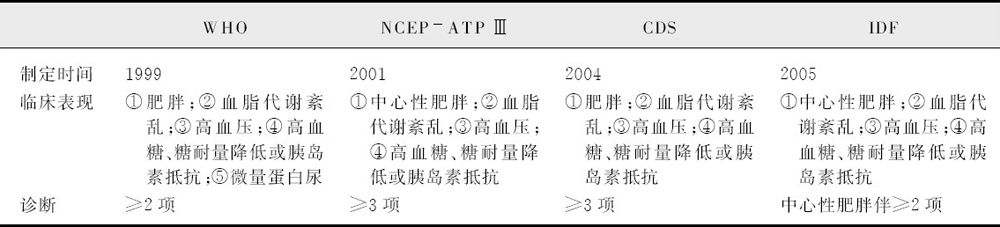
\includegraphics{./images/Image00043.jpg}
\end{table}

\hypertarget{text00004.htmlux5cux23mllj32}{%
\subsection{NAFLD的诊断}\label{text00004.htmlux5cux23mllj32}}

NAFLD诊断及定量研究的金标准是肝活检,但临床应用受到限制。目前常用方法为B型超声、CT、MRI等。中华医学会肝脏病学分会脂肪肝和酒精性肝病学组所制定NAFLD的诊断标准包括:①有易患因素:如肥胖、2型糖尿病、高脂血症,或胰岛素抵抗;②无饮酒史或饮酒折合酒精量<40g/周;③除外病毒性肝炎、药物性肝病、Wilson病、全胃肠外营养和自身免疫性肝病等;④除原发疾病临床表现外,可出现乏力、肝区隐痛等症状,可伴肝、脾肿大,但绝大多数病人无任何症状,仅在体检中发现存在脂肪肝;⑤血清转氨酶可升高,并以ALT升高为主,可伴有GGT、铁蛋白和尿酸等增高;⑥肝脏组织学有典型表现;⑦有影像学诊断依据。

{1.单纯性脂肪肝}
 凡具备下列第1~2项和第3或第4任何一项者即可诊断:①具备临床诊断标准1~4项;②肝功能检查基本正常;③影像学符合轻、中度脂肪肝;④肝脏组织学表现符合单纯性脂肪肝,无明显肝内炎症和纤维化。

{2.非酒精性脂肪性肝炎}
 凡具备下列第1~2项和第3或第4任何一项者即可诊断:①具备临床诊断标准1~4项;②血清ALT和(或)GGT高于正常值上限1.5倍,持续时间>4周;③有影像学诊断依据;④肝脏组织学诊断证实。

{3.脂肪性肝纤维化和(或)肝硬化}
 凡具备下列第1~2项和第3或第4任何一项者即可诊断:①具备临床诊断标准1~4项;②肝功能和血清纤维化标志可正常或异常;③影像学提示脂肪肝伴肝纤维化或肝硬化;④肝脏组织学诊断证实。

\hypertarget{text00004.htmlux5cux23mllj33}{%
\subsection{治疗}\label{text00004.htmlux5cux23mllj33}}

根据NAFLD发病机制及其伴随的高危因素,目前应采用综合治疗,包括营养、运动、健康教育(行为和心理)、药物(胰岛素增敏剂、降脂药物、抗氧化剂和肝细胞膜保护剂等)4个方面。

(一)营养治疗

对于肥胖伴NAFLD病人通过控制总能量摄入,建立和培养合理三大产能营养素结构比,促使病人减轻体重和BMI,达到降低血ALT水平,改善肝脏组织学形态的目的。国内朱惠娟等报道通过1年减重治疗,45例肥胖伴NAFLD病人BMI平均降低3.0kg/m\textsuperscript{2}
,病人血浆ALT水平明显降低,65.7%的病人肝脏组织学形态得到明显改善。万燕萍等对58名肥胖儿童伴NAFLD采用营养(高蛋白质、适量脂肪和碳水化合物模式)和体育锻炼为主的综合疗法,同时补充B族维生素和微量元素硒,治疗时间为3~18个月(平均7.1个月),结果显示随着BMI的降低,65.5%的患儿肝脏形态恢复正常,29.3%的患儿出现明显改善,仅有5.2%的患儿肝脏形态无明显改善。

{1.营养治疗原则}
 营养治疗的原则是根据病人理想体重,给予适量能量,合理分配三大产能营养素比例,适当补充维生素、无机盐及膳食纤维,改变不良饮食习惯,同时兼顾运动和健康教育(行为和心理)。营养治疗时应教会病人及家属应用食品交换份,合理实施营养计划。营养治疗目标是尽可能维持理想体重、控制血脂和血糖在正常范围、防止或改善慢性代谢性并发症、保证三大产能营养素和微营养素的需要量、维持机体正常的生理功能和社会活动。通过饮食控制使体重每月下降1~2kg,达到减重目标后给予维持量。肥胖儿童伴NAFLD病人能量控制不必太严格,在保证儿童生长发育时,维持原有体重或使体重略有降低,即可达到BMI降低的目的。理想体重计算公式为身高(cm)-105或身高(cm)-100×0.9。

{2.营养治疗措施}

(1)能量:能量供给应根据病情、病程、年龄、身高、体重、劳动强度和活动量而定,一般根据理想体重进行计算,对于肥胖卧床病人,每天能量应≤63kJ/(kg·d)[15kcal/(kg·d)],轻度体力活动15~20kcal/(kg·d),中等体力活动20~25kcal/(kg·d),重度体力活动为25~30kcal/(kg·d)。儿童总能量应能保证正常生长发育,一般6~9岁为4184~5858kJ/d(1000~1400kcal/d);10~14岁为5021~6694kJ/d(1200~1600kcal/d);15~18岁为5858~7531kJ/d(1400~1800kcal/d)。轻、中度肥胖儿取上限值,重度肥胖儿取下限值。

(2)产能营养素比例:在控制总能量摄入的基础上,通过合理调整三大产能营养素的比例、增加维生素、微量元素、膳食纤维的摄入可通过降低体重和BMI,进而降低NAFLD的发生。碳水化合物、脂肪、蛋白质占总能量的百分比分别为45%~55%、25%~30%、15%~25%。由于肥胖病伴脂肪肝病人常有脂质代谢紊乱,以往多采用低脂饮食模式对病人进行治疗,但如今的研究证实低脂饮食模式可能并不适合用于治疗脂肪肝。对脂肪肝病人仍应给予适量的必需脂肪,才能保证脂肪从肝脏顺利运出,有利于NAFLD治疗。碳水化合物摄入过多可能通过增加三酰甘油合成、降低脂肪廓清使血脂水平升高。低碳水化合物饮食较低脂肪饮食对改善脂肪肝病人血脂代谢和降低体重的作用更加明显。Foster等人将治疗63例肥胖病人随机分为两组,治疗组应用Atkins模式(低碳水化合物、高蛋白质、高脂肪),对照组使用常规模式(高碳水化合物、低脂肪、低能量),6个月后治疗组病人体重和血TG下降程度较对照组更加明显,HDL-C则明显升高,胰岛素敏感性明显改善。碳水化合物和蛋白质比例降低还可降低肥胖病人体内脂肪含量,血TC和TG水平明显降低。万燕萍等使用高蛋白质、适量碳水化合物和脂肪模式(三者比例为20%~25%、45%~50%和25%~30%)治疗儿童、青少年肥胖伴脂肪肝已取得满意疗效,总有效率可达95%。与国外学者使用的营养治疗方案相比,万燕萍等使用的方案虽然总能量有所增加,但碳水化合物降低,脂肪和蛋白质用量增加,增加的脂肪和蛋白质主要以牛奶、鱼及海鲜为主,这些食物以优质蛋白质、单不饱和脂肪酸及磷脂为主,提高这些营养素的摄入可在降低体重的同时保证机体生长发育和瘦体组织群的正常代谢。同时,该作者认为高蛋白质饮食可提高血中磷脂酰胆碱和肉毒碱水平,有利于长链脂肪酸氧化,减少肝脏中三酰甘油堆积。适量碳水化合物摄入则降低肥胖患儿血胰岛素水平,抑制脂肪酸再酯化,使脂肪合成减少。

在调整三大产能营养素比例的同时,还应注意脂肪和碳水化合物种类。适当提高单不饱和脂肪酸(橄榄油、茶油)和多不饱和脂肪酸比例,降低饱和脂肪酸摄入有利于改善NAFLD病人糖脂代谢,因而有利于NAFLD的治疗。分子结构相对复杂的多糖如支链淀粉等相对于单糖和双糖而言,病人餐后血糖更加平稳。

(3)坚持培养合理饮食和生活习惯:实行有规律的一日三餐,避免暴饮暴食和夜宵,减少快餐和零食。饮食方式不规律,如经常不吃早餐,或三餐分配不均都可扰乱体内物质代谢。合理餐次能量分配为早∶中∶晚=25%∶40%∶35%。

增加膳食纤维摄入量。根据病人耐受情况,每天膳食纤维摄入量可在25~40g之间。

(4)维生素:添加B族维生素具有减少自由基产生、调节血脂的功能。10\textsuperscript{-6}
~10\textsuperscript{-4} mol/L维生素B\textsubscript{1}
即可明显抑制体外培养的肝脏细胞微粒体脂质过氧化,减少自由基产生。B族维生素不仅可以减少自由基产生,作为物质代谢的辅酶之一,B族维生素对物质代谢的调节至关重要,缺乏B族维生素可能损伤肝脏对营养物质的代谢能力,而肝脏对营养物质代谢能力的改变是脂肪肝发生的重要因素之一。维生素A和β-胡萝卜素可防止肝纤维化,维生素C具有抗氧化功能。补充足量的维生素有助于预防NAFLD。

维生素E对NAFLD的作用仍存在争议。有学者认为给予NAFLD/NASH病人维生素E,即使体重没有明显改善或降低,单独应用维生素E也可降低血清ALT和AST水平。反对观点认为给予维生素E没有明显作用,血清肝酶指标的降低和肝脏组织学的改善主要得益于BMI和IL-6的降低。鉴于维生素E对NAFLD的作用仍不明确,且一项Meta分析结果显示补充维生素E超过400IU/d后死亡率增加,因此我们不推荐常规补充维生素E。

(5)食盐:食盐摄入过多可引起口渴和刺激食欲并增加体重,故每天摄入量应<6g。

(6)茶叶:茶叶是一种低能量食物。种类的不同茶叶能量不同。绿茶提供的能量最高(300~350kcal/100g),红茶、花茶、乌龙茶等次之,砖茶最低。茶叶中成分比较复杂,目前已知对人体有利的营养成分有茶氨酸、多糖、维生素C、无机盐、微量元素、生物碱、茶多酚等。已有研究证实饮茶可以减轻体重和体内脂肪储存、降低肝脏脂肪酸合成、抗氧化等多种功能,因而可能应用于NAFLD治疗。

(7)其他营养物质:部分营养物质与NAFLD发生关系密切。目前已有研究所涉及的病例数较少,因而应用这些营养物质是否能够有效预防和治疗NAFLD还需进一步研究。

1)硒:硒是人体必需的微量元素,硒与脂肪肝病人脂质代谢、脂质过氧化密切相关。缺硒可导致LDL-C、TG和TC合成增加。补充硒可以促进谷胱甘肽过氧化物酶合成,保护人体免受自由基的侵害;还可改善肝细胞结构和功能,阻止肝纤维化的产生。动物实验中发现,补硒可显著降低高脂血症大鼠血清TG,升高HDL-C水平;补硒组大鼠血浆谷胱甘肽过氧化物酶和超氧化物歧化酶活性明显升高。肝脏病理切片亦显示补硒组大鼠肝脏脂肪变性程度明显减轻。

2)S-腺苷蛋氨酸:S-腺苷蛋氨酸(S-adenosylmethionine,
SAMe)是条件必需氨基酸,可以保护细胞膜稳定性、促进VLDL和GSH合成。口服S-腺苷蛋氨酸可以升高酒精性肝炎、肝硬化病人血浆和肝脏内GSH含量。

3)肉毒碱(carnitine):79例NAFLD病人应用左卡尼汀治疗4周,减量后继续治疗4周,显效64例(81.0%),有效9例(11.4%),总有效率为92.4%。左卡尼汀还能显著降低2型糖尿病伴高胆固醇血症病人的脂蛋白水平,改善脂质代谢。

4)甜菜碱:甜菜碱(betaine)是胆碱的代谢产物之一。动物实验表明口服1%浓度的甜菜碱可以减轻高蔗糖饮食造成的肝脏脂肪浸润。人体实验表明口服甜菜碱1年可使NASH病人血清ALT水平降低或恢复正常,脂肪变性、炎性坏死和纤维化程度得到明显改善。

5)益生菌(probiotics)和益生元(prebiotics):内毒素对肝细胞有直接毒性作用,可引起肝脏能量代谢紊乱。内毒素还可以促进细胞因子的释放和炎症介质的产生,扩大内毒素作用。膳食纤维、益生菌和益生元均可有效维持肠道黏膜屏障,减少细菌移位和内毒素产生等作用,因而认为膳食纤维、益生菌和益生元等可能有助于预防NAFLD的发生。

6)牛磺酸:19例经B超和(或)CT证实的NAFLD病人,服用牛磺酸(6.0g,分3次餐后服用),12周后牛磺酸治疗病人血ALT、AST、γ-GT显著降低,空腹血糖、TC和TG也有明显下降,B超或CT检查脂肪肝程度得到一定程度改善。动物实验亦证实牛磺酸可能减轻肝脏脂肪变性程度。

(二)运动

运动的重要性仅次于营养治疗,最适合肥胖和伴有胰岛素抵抗的NAFLD病人。运动不但使能量消耗增加,还可减少因单纯低能量饮食造成的蛋白质丢失,促使更多脂肪分解,并增强体质,降低血压、血脂、体重,控制血糖。在实施运动治疗前,应根据病人的实际情况和可能并存的疾病,注意结合病人爱好,以及原有运动基础、肥胖度、体重、年龄等选择不同运动方式,将安全、有效、兴趣结合,达到消耗能量、降低体重和BMI、改善胰岛素抵抗的目的,从而逆转NAFLD。营养和运动相结合可大大提高NAFLD病人的治疗效果。运动强度应以运动后劳累程度和心率进行界定,以运动时心率100~160次/分(或运动时心率=170-年龄),持续20~30分钟,运动后疲劳感10~20分钟后消失为宜。

(三)健康教育

短期严格的营养和运动治疗可有效降低NAFLD病人体重和BMI,改善病人血糖和血脂水平,降低ALT水平,从而达到改善肝脏组织学形态的目的。问题的关键在于,有相当多的病人在治疗后出现“复发”现象。健康教育通过让病人了解疾病的病因、发病机制和危险因素,纠正和改变与NAFLD相关的不良饮食和行为习惯,达到防治疾病、巩固治疗效果的目的。让病人认识到肥胖或脂肪肝与自己的不良行为有关,有助于增强病人治疗成功的信心,提高病人坚持治疗的依从性。通过行为和饮食日记,详细记录NAFLD病人每天的饮食摄入量、膳食结构比例、烹调方法、运动量等,有助于在以后的随访过程中可以不断的指导和纠正,提高治疗的效果。

(四)药物

主要包括降脂药物、细胞膜保护剂、抗氧化剂、胰岛素增敏剂以及中药等。

综上所述,科学合理的营养治疗在NAFLD的防治中起着相当重要的作用,其效果往往优于药物治疗。但要获得最佳的治疗效果,还需与病因治疗、运动与健康教育等相结合。

\hypertarget{text00004.htmlux5cux23mllj34}{%
\section{ 营养与骨质疏松症}\label{text00004.htmlux5cux23mllj34}}

骨质疏松症(osteoporosis)是老年人的常见病。随着世界人口的老龄化趋势,老年人比例增加,其发生率逐渐上升。骨质疏松导致的骨痛、骨折、脊柱畸形和活动限制等病例已很常见。骨质疏松症的防治越来越受到大家的关注,预防骨质疏松症重要的是学会科学的饮食和锻炼。

\hypertarget{text00004.htmlux5cux23mllj35}{%
\subsection{发病机制及诊断}\label{text00004.htmlux5cux23mllj35}}

(一)定义

骨质疏松症是一种低骨量和骨组织微结构受损、骨质无机盐成分及骨基质等比例不断地减少、骨质变薄、骨小梁数量减少、骨骼脆性增加、容易发生骨折的全身性疾病。

(二)病因

骨质疏松症的病因还不完全清楚,以下几个因素在该病的发生、发展过程中起着重要作用。

{1.遗传因素}
 骨密度及骨代谢与遗传因素有关,对孪生子的研究表明,70%骨量取决于遗传因素。随着年龄的增长,骨质疏松的发生受环境因素的影响逐渐加大,而遗传因素的影响逐渐减弱。

{2.营养失衡}
 长期钙摄入不足、维生素D缺乏及长期进食高纤维素的食物及厌食、偏食习惯的人都有可能发生骨质疏松症。

{3.机械因素}  肢体废用、肢体长期固定、不负重,均可引起局部骨质疏松。

{4.疾病因素}
 很多骨关节病变,如骨关节结核、类风湿关节炎、化脓性关节炎,或某些骨肿瘤可引起病灶周围弥漫性继发性的脱钙和骨质疏松。

{5.不良嗜好}  长期酗酒、吸烟及嗜食含咖啡因的食物如咖啡、浓茶、可乐等。

{6.服用某些药物}
 长期服用某些药物如类固醇激素、利尿剂、抗生素、抗血液凝固剂及接受化疗等。

{7.激素失调}
 中老年人性激素(雌激素)分泌减少、钙调节激素(甲状旁腺激素,降钙素)分泌失调,使骨代谢紊乱。

(三)发病机制

{1.骨的结构与功能}
 骨骼系统包括骨、软骨及附属结构,有着重要的生理功能。骨骼系统构成机体坚硬的骨架结构,并构成一定形状的腔隙保护人体的重要器官;骨和关节是运动系统的主要组成部分;骨骼腔内的骨髓是主要的造血器官;骨是体内钙和磷的储存库,调节钙、磷代谢。骨骼由外层致密的皮质骨和内层小梁骨(松质骨)构成。皮质骨占骨总量的80%,主要位于长骨骨干,松质骨占20%,位于脊椎、骨盆和骨的干骺端。骨组织中细胞占2%~5%,其中重要的是骨细胞,包括成骨细胞和破骨细胞。骨矿物质约占成人骨干重的65%,其中钙占37%~40%,磷占50%~58%,磷酸盐占2%~8%,此外还有少量钠、钾、镁等。骨的有机质中主要是骨胶原,它占有机成分的90%。还有一类非胶原蛋白质,约占10%,如骨钙蛋白,具有一些重要的生物活性。

{2.骨重建过程}
 骨的新陈代谢非常活跃。骨发育成熟后,在一生中不断进行骨重建,以保持骨组织的自身修复。骨重建过程,首先是骨吸收,破骨细胞分泌溶酶体酶,移去一定量的骨组织。骨吸收阶段为1~3周。骨吸收完成后1~2周,骨形成才开始,包括类骨质的合成与分泌及类骨质的矿化两个阶段。骨重建周期持续2~3个月,但老年人可达6个月。在稳定状态下,骨吸收量等于骨形成量。

{3.骨量的获得与丢失}
 人一生中骨量变化分为三个阶段:第一阶段为骨量上升期,出生后骨量不断增长,在30~35岁达到骨峰值;第二阶段为骨代谢平衡期,女性自30~50岁(绝经期),男性自30~70岁;第三阶段为骨量减少期。青春期是骨量发育的关键时期。

{4.骨峰值}  骨峰值越小,越容易发生骨质疏松症。

(四)分类

{1.原发性}
 Ⅰ型(绝经后骨质疏松)最常见于绝经不久的女性(多在51~65岁),为高转换型,即骨吸收和骨形成均很活跃,但以骨吸收为主,多见脊柱和桡骨远端;Ⅱ型(老年性骨质疏松)多见65岁以后的老年人,为低转换型,即骨吸收和骨形成均不活跃,但仍以骨吸收为主,主要侵犯椎体和髋骨及长管状骨干骺端。原发性老年型骨质疏松的患病率男性为60.72%,女性为90.47%。

{2.继发性}
 常继发于其他疾病或长时间服用某些药物,如内分泌代谢性疾病(甲状旁腺功能亢进症,库欣综合征,甲状腺功能亢进症,性腺功能减退症,糖尿病),血液病(骨髓瘤,白血病),胃肠道疾病,长期卧床、制动等;药物如类固醇激素等。

{3.特发性}  多见于8~14岁的青少年,多数有遗传家族史,女性多于男性。

(五)临床表现

骨质疏松症早期可以没有明显的临床症状和体征,到中期以后则会出现疼痛、身高变矮、驼背、骨折及呼吸系统障碍。

{1.疼痛}
 是原发性骨质疏松症最常见、最主要的症状,当骨量丢失12%以上时即可出现骨痛,以腰背痛为多见,占疼痛病人的70%~80%,疼痛沿脊柱向两侧扩散,晨起时最明显,弯腰、肌肉运动、咳嗽等时加重,以后腰背痛可转为持续性。其他依次为膝关节、肩背部、手指、前臂、上臂,主要是由于骨转换过快,骨吸收增加,骨小梁破坏、消失及骨膜下皮质骨的破坏所引起。

{2.身长缩短驼背}
 多在疼痛后出现。脊椎椎体前部几乎多为松质骨组成,而且此部位是身体的支柱,负重量大,尤其第11、12胸椎及第3腰椎,骨质疏松时椎体骨量丢失明显,骨小梁变细,数量减少,强度减弱,易致椎体变形,使脊椎前倾,背曲加剧,形成驼背。随着年龄增长,骨质疏松加重,驼背曲度加大,致使膝关节挛拘显著。正常人每一椎体高度约2cm,老年人骨质疏松时椎体压缩,每一椎体缩短约2mm,身长平均缩短3~6cm。

{3.骨折}
 是退行性骨质疏松最常见和最严重的并发症,它不仅增加病人痛苦,加重经济负担,并严重限制病人活动,甚至缩短寿命。据我国统计,老年人骨折发生率为6.3%~24.4%,尤以高龄(>80岁)女性老人为甚。骨质疏松性骨折多由轻度外伤引起,一般骨量丢失20%以上时易发生骨折。骨折好发部位是胸腰椎体、桡骨远端和股骨颈部位。髋部骨折危害最大,据报道50%会致残,病死率可达10%~20%。椎体骨折可引起驼背和身材变矮。

{4.呼吸功能下降}
 胸、腰椎压缩性骨折,脊椎后弯,胸廓畸形,可使肺活量和最大换气量显著减少,病人往往可出现胸闷、气短及呼吸困难等症状。

(六)诊断

{1.影像学检查}

(1)X线摄片检查:X线为一种较易普及的检查骨质疏松症的方法。但该方法只能定性,不能定量,且不够灵敏,一般在骨量丢失30%以上时,才能有X线阳性所见。表现为骨皮质变薄、骨小梁减少或消失、骨小梁的间隙增宽、骨结构模糊、椎体双凹变形或前缘塌陷呈楔形变等。

(2)超声波(USA):可测定骨密度和骨强度。与DXA法相关性良好,该法操作简便、安全无害、价格便宜,值得推广。

(3)双能X线吸收测定法(DEXA):通过X线束滤过式脉冲开头技术可获两种能量,即低能和高能光子峰。射线穿透身体之后,扫描系统将接受的信号传送到计算机进行数据处理,计算骨矿物质含量(BMC)、面积(AREA)、BMD。该仪器可测定全身任何部位的骨量,精确度可达到0.62%~1.3%。对人体危害较小。此法较准确、重复性好,在我国各大城市已逐渐开展。

{2.骨活检}
 各种无创伤性的骨密度测定仅能反映全身或局部的矿化骨含量,而骨活检能较准确地了解骨和前骨质的量、质、结构、骨细胞的数目、功能及骨转化和重建情况。故骨活检作为一种安全易行、创伤小的检查方法,在临床和科研中仍有不可替代的作用。

{3.实验室检查}

(1)碱性磷酸酶(AKP):AKP为成骨细胞合成和分泌,AKP活性高可反映成骨细胞活跃,测同功酶骨AKP较敏感。骨更新率增加的代谢性骨病如畸形骨炎、先天性佝偻病、甲状旁腺功能亢进、骨转移癌及氟骨症等显著升高。绝经后妇女骨质疏松症约60%骨AKP升高,老年骨质疏松骨AKP变化不显著。

(2)血浆抗酒石酸盐酸性磷酸酶(TRAP):主要由破骨细胞释放,是反映破骨细胞活性和骨吸收状态的敏感指标,老年性骨质疏松症TRAP增高不显著。

(3)血、尿骨矿物质成分的检测

A.血清总钙:正常人血清总钙值2.1~2.75mmol/L(8.5~11mg/dl),老年性骨质疏松症血钙一般在正常范围。

B.血清无机磷:正常成人血清无机磷总量是0.87~1.45mmol/L(2.7~4.5mg/dl),儿童1.45~1.78mmol/L(4.5~5.5mg/dl)。绝经后妇女骨质疏松症血磷上升,老年性一般正常。

C.血清镁:肠道对镁的吸收随着年龄增长而减少,绝经后及老年性骨质疏松症血清镁均下降。

D.尿钙、磷、镁的测定:是研究骨代谢的重要参数,通常测定包括24小时尿钙、磷、镁,每克肌酐排出的尿钙、磷比值。老年性骨质疏松症尿钙、磷在正常范围,尿镁略低于正常范围。

\hypertarget{text00004.htmlux5cux23mllj36}{%
\subsection{骨质疏松症的防治}\label{text00004.htmlux5cux23mllj36}}

(一)药物治疗

当前,在骨质疏松症的药物治疗上,大致可分为两大类:一类为抑制骨质流失,为当今治疗的主流;另一类为促进骨骼成长,当前尚无令人满意的结果。

{1.抑制骨质流失药物}

(1)钙制剂:钙元素在中、老年人中可经由抑制副甲状腺素而达到抑制破骨细胞及骨代谢的作用。且钙质也是构成骨骼的主要成分之一。钙质的摄取最好注重于天然食品补充,如奶制品、小鱼干、发菜等。若饮食摄取不足,可考虑服用钙片。钙剂分三大类:无机钙如碳酸钙等,在体液中溶解度低;有机酸钙如乳酸钙、葡萄糖酸钙等;有机钙如氨基酸螯合钙等。后两大类在体液中溶解度较高。

根据不同年龄和疾病而选择不同钙剂。缺乏胃酸者基本不吸收无机钙,因此建议>65岁、<3岁和胃酸缺乏者服用有机酸钙如枸橼酸钙。足量补充钙,提高骨峰值以预防骨质疏松症。骨峰值以后,即35岁以后应常规补钙,以维持钙的平衡和骨密度的稳定。

(2)维生素D:维生素D的最主要作用是帮助小肠对钙的吸收,但对骨细胞的成熟与功能也有作用,老年人即使是使用小量的未活化型维生素D与钙片,有报道显示其骨密度的减少趋缓,骨折率减少。

对于日照少的地区和绝经晚期妇女可适当补充维生素D400IU/d或活性维生素D\textsubscript{3}
帮助钙的吸收和利用,但单用维生素D不能减少骨折的发生率。

(3)雌激素:雌激素通过成骨细胞内的受体,调解成骨细胞分泌特殊的介质,来抑制破骨细胞。女性停经后的快速骨量减少,与雌激素的快速消减有关。雌激素对骨骼的保护作用,于停经后约15年内效果最大,其后骨骼不再快速流失,效果就减少。

(4)降钙素:临床上使用的是鱼类的降钙素,包括鲑鱼降钙素(密盖息)及鳗鱼降钙素(益盖宁),鱼降钙素可直接抑制破骨细胞,减少骨骼的流失;另外它可经神经系统的感受器,减少疼痛的强度,所以对防止骨质疏松症及骨折的疼痛都有效果。其不良反应少,少数人只有恶心、潮热红或手痒等症状。

(5)双磷酸盐类:二磷酸酐类药物(bisphosphonate)基本结构为-P-C-P,为焦磷酸酐-P-O-P的衍生物。其基本作用在于抑制破骨细胞,以及抗拒各种磷酸的消化,所以可对抗破骨作用。目前制剂有福善美(Forsamax)等。

{2.造骨性药物}

(1)氟化物:氟离子可直接刺激造骨细胞,促进骨骼的造骨作用。较小剂量使用,可一方面增加骨骼的量,一方面骨骼代谢不至太快而造成不好的影响。氟化物当前在治疗骨质疏松症的地位尚未确定。

(2)副甲状腺素:以间接性皮下注射法,在人体及动物可见到骨骼量略为增加。当前已有副甲状腺素上市,但仅供临床试验用,用于治疗目的尚待研究。

(3)同化类固醇:同化类固醇(anabolic
steroids)因刺激骨骼形成,增加血色素及增强肌力,故被用于年老的严重病人,或因缺乏男性激素的男性骨质疏松症病人。

(4)周期性或Cohort疗法:ADFR处方,这是一种理论性的治疗骨质疏松症的良方,最先由Frost所提出。首先以一些药物,如活性维生素D\textsubscript{3}
、或PTH、或甲状腺素刺激骨骼进入活动期,继而在活动期骨溶解作用减缓进行,接着骨代谢周期会进入骨形成阶段,共约3个月(100天),整个骨代谢过程完成,再重复以上治疗。

以上两大类药物,在临床上可合并使用。大多数病人均应使用钙片,停经期前后的妇女应多考虑使用雌激素,老年女性骨质疏松严重病人,如不愿使用雌性激素或是使用有不良反应者,可以考虑使用双磷酸盐类,特别是福善美,乳癌病人又有骨质疏松症时,双磷盐类也是较好的选择,如有脊椎压迫性骨折合并疼痛者可优先考虑降钙素使用。

(二)营养与骨质疏松症

{1.钙}
 钙缺乏引起骨质疏松的机制主要由于低钙摄入使血钙降低,继发性PTH分泌增加,血PTH升高,骨吸收增强,骨钙被动员进入血液以保持血钙正常,若长期摄钙不足,则骨钙不断流失,导致骨量减少,引起骨质疏松。反之,细胞外钙离子浓度增高能加速破骨细胞的凋亡,抑制破骨细胞的功能,骨吸收明显下降。

{2.维生素D}
 维生素D对骨矿物质代谢的影响是双向的。一方面是维生素D促进骨形成。成骨细胞上有1,25-(OH)\textsubscript{2}
D\textsubscript{3}
的受体,是维生素D作用的重要靶细胞,1,25-(OH)\textsubscript{2}
D\textsubscript{3}
可促成骨细胞合成骨钙素等,使骨组织胶原的矿化,这是维生素D对骨形成的直接作用;另外,肠黏膜细胞中亦有1,25-(OH)\textsubscript{2}
D\textsubscript{3}
的受体,尤以十二指肠最多,1,25-(OH)\textsubscript{2}
D\textsubscript{3}
诱导小肠上皮合成钙结合蛋白,其与钙离子有较大的亲和力,一分子钙结合蛋白结合2个钙离子可促进钙吸收。另一方面,破骨细胞的前体细胞上也有1,25-(OH)\textsubscript{2}
D\textsubscript{3} 的受体,1,25-(OH)\textsubscript{2}
D\textsubscript{3}
也能促进前体细胞分化而增加破骨细胞的数量,引起骨吸收增加,这是维生素D的负性调控。骨骼肌是活性维生素D代谢的靶器官,维生素D缺乏时可出现肌无力、肌肉收缩和松弛功能的异常,从而增加跌倒的机会,增加了骨折的发生率。

{3.磷}
 日常的饮食结构中含有丰富的磷,所以磷的摄入很少有不足,往往是过度的磷摄入。高磷摄入使血磷偏高,可引起骨盐丢失,当钙、磷乘积<35时骨矿化迟缓。

{4.维生素K与骨钙素}
 早在1975年Peffifor和Benson发现服抗凝剂(维生素K拮抗剂)的怀孕妇女,其所产婴儿有骨骼畸形,首次揭示了维生素K缺乏对人体骨骼发育的影响。骨钙素是一种低分子量蛋白质,其分子中3个谷氨酸残基在维生素K依赖性羧化酶的作用下,羧化为γ-羧化谷氨酸。γ-羧化谷氨酸与骨的无机成分羟基磷灰石中的钙离子结合。维生素K缺乏时,一部分谷氨酸残基未能形成γ-羧化谷氨酸,因而与羟基磷灰石结合力低下,影响骨骼的正常钙化。

{5.蛋白质}
 关于蛋白质摄入与骨健康关系的研究报道有两种相反的结果,目前尚没有足够的证据提出为预防骨质疏松症的蛋白质的适宜摄入水平。哈佛大学营养学教授沃尔特·威廉证实:动物性蛋白质的摄取量越多,钙质排出体外的机会就相对增加,很容易引起钙缺乏症。实验证明,每天摄入80g动物蛋白质,会造成37mg的钙流失;当蛋白质的摄入量增加到每天240g,这时即使再补充1400mg的钙,最后总的钙流失还是会达到每天100mg左右。因为含硫的动物性蛋白质进入人体后,会使血液呈酸性反应,逼迫身体从骨质中提取钙质来平衡酸性血液;红肉中含有大量的磷酸根,会在消化道中与钙结合,从而减少人体对钙的吸收;食物中的钙经过消化,变成游离钙才能被小肠吸收,红肉中饱和脂肪酸含量高,会在胃肠道与钙结合,形成不溶性脂肪酸钙,使钙的吸收率降低。但Framingham在对600多名平均75岁的老年人的膳食调查结果表明:蛋白质摄入低者髋部及脊椎骨钙丢失均显著高于蛋白质摄入高者,且低蛋白质组骨折率也较高。

{6.其他}
 镁是体内重要矿物质,人体60%~65%的镁存在于骨和牙组织,镁可增强维生素D活性,而低镁可影响维生素D活性;赖氨酸和精氨酸也可促进钙的吸收,增强结缔组织,并能刺激生长激素的分泌,加强骨细胞的增长;维生素C促进骨的形成期及钙质的吸收;葡萄糖胺促进骨骼和结缔组织的健全发展;硫也能够增强骨骼。反之,草酸会抑制人体对钙质的吸收。

(三)预防

亚洲食品信息中心认为,要想预防骨质疏松,必须达到3个关键的目标:通过膳食摄入足量的钙;保证机体从膳食或通过太阳获得足量的维生素D;每天规律地进行锻炼。

{1.饮食}

(1)科学补钙:食物补钙最为安全,也容易被人体接受。

1)牛奶:牛奶是最好的钙质来源。许多研究显示,钙质和乳酸结合成乳酸钙时,人体较容易吸收,而牛奶中就含有许多的乳酸钙。对乳糖不耐受者,可以选用硬奶酪(如瑞士奶酪)、酸奶和一些特殊加工的低乳糖食品。

由于中国妇女饮食钙摄入较少(平均<500mg/d)。在香港进行对照试验显示:服用高钙奶(800mg/d)2年,骨质丢失显著减少。

2)豆制品:豆腐和黄豆制品除了含有丰富的钙质外,还含有一种叫做异黄酮的物质,可以降低骨破坏,增加骨形成和骨密度。

3)带壳食物:这些食物往往富含钙。虾、蟹等动物肉本身也有一定钙含量,如能嚼壳一起吃,吃进去的钙就更多;花生、瓜子、杏仁等虽壳不能吃,但是这些坚果一样富含钙质。

4)其他:海藻类食物如紫菜、海带等含有许多的钙质;绿色蔬菜也含比较丰富的钙,但一些蔬菜如菠菜、芦笋等因含草酸较多,与牛奶、豆腐等一起使用会妨碍钙的吸收。

5)适量醋:适量的酸性食物有利于钙吸收。

表3-27为可提供钙150~200mg的一些食物估计量。

\begin{table}[htbp]
\centering
\caption{下列食物可提供钙150~200mg}
\label{tab3-27}
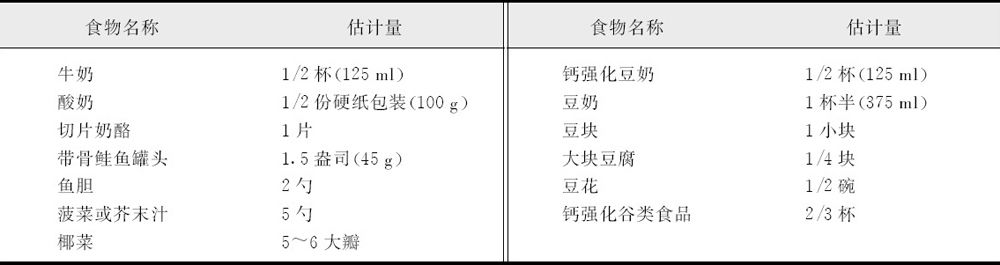
\includegraphics{./images/Image00044.jpg}
\end{table}

(2)维生素D:维生素D调节钙、磷代谢,促进钙、磷吸收和骨胶原合成。富含维生素D的食物,如鱼肉、奶油、蛋、肝、牛奶等;在户外晒太阳,也能增加体内维生素D的摄取量。

(3)蛋白质:适量的蛋白质可增加钙的吸收和储存,有利于骨的再生和延缓骨质疏松的发生。选用优质的动物蛋白和植物蛋白,如新鲜的鱼类、蛋奶制品和豆制品。

(4)维生素C:维生素C有利于钙的吸收和向骨骼中沉积。故应多吃新鲜的水果和蔬菜,如柳橙、芒果、奇异果、番茄、芥蓝、菜心等。

(5)少吃盐:盐里所含的钠,其排泄过程伴有钙的流失。尽量将每天的食盐摄入量控制在5g以下,减少酱油(5ml酱油相当于1g盐)、味精、鸡精等调料用量,少吃或不吃盐渍或腌制肉、酱菜、咸菜以及咸味零食物。

(6)多摄钾:膳食中增加钾的摄入,可促进钙吸收,缓解骨溶解。钾的推荐摄入量为每天2000mg,蔬菜、水果、豆类、奶制品以及肉、禽、鱼等食物中钾含量很高,达到推荐量并不难。

(7)适量磷:磷在食物中来源广泛,缺磷者极为罕见。临床上磷耗竭症状仅见于全胃肠外营养长期使用而未添加磷制剂的病人,慢性病、肠炎或手术肠吸收面积大量丧失的病人及大剂量服用氢氧化铝的病人。但是,高磷摄入可引起骨盐丢失。

(8)加镁饮食:若每天增加100mg镁的摄入,全身骨密度增加约2%,每天镁的推荐摄入量为350mg。绿叶蔬菜、粗粮、坚果、蘑菇、海带等含镁较高,但并不越多越好,不应超过700mg。

(9)避免高脂食物、抽烟、饮酒,以及喝咖啡、浓茶等刺激性饮料。

(10)避免草酸:食用菠菜、苋菜的含草酸蔬菜时,烹饪前最好在80℃以上的热水中焯一下,将菠菜中草酸清除后再食用。

{2.运动}
 只有配合适当的运动和充足的日晒,才能将这些钙的作用“激活”,达到预防骨质疏松的目的。体育锻炼也可以促进新陈代谢和全身的血液循环,增强骨组织对所需的营养,特别是对钙的吸收,有效提高骨质的硬度和韧性。经常锻炼的青少年老年后患骨质疏松的时间较晚,病情也较轻。运动对于老年人同样必不可少。强健的背部肌肉可减少驼背和椎骨骨折的发生,适量运动有助于保持甚至提高骨密度。运动还可提高老年人身体的协调性和平衡能力、减少跌倒的风险,降低各种骨折的发生率。一项研究表明,常打太极拳与不打太极拳的人相比,跌倒的概率可减少47%,髋部骨折率可降低25%。

运动是防治骨质疏松症的良方。快走、爬楼梯、跳舞、打球、打太极拳、游泳等都是较好的锻炼方式,随时随地可以进行锻炼的几个简单动作如:金鸡独立、踮起脚跟、单脚跳等,生活间隙也可做些类似广播体操的肢体运动,但对于老年人,尤其合并心脑血管慢性疾病的病人,运动应注意循序渐进、持之以恒,要避免过度超负荷的运动。

{3.WHO针对骨质疏松性骨折提出的建议}

(1)针对骨质疏松性骨折的一些建议:高骨折发生率的国家,要求最少每天应摄入400~500mg的钙以预防骨质疏松。当乳制品摄入有限时,其他的钙来源应包括骨头能吃的鱼、用钙处理过的玉米饼、钙含量高的绿色蔬菜(如花茎甘蓝和羽衣甘蓝)、豆类、豆制品(如豆腐)。在建议低骨折发生率国家的人群增加钙摄入量前,需要考虑到钙摄入量与体力活动、日晒以及其他膳食成分(如维生素D、维生素K、钠和蛋白质)和有保护作用的植物营养素(如大豆化合物)的摄入量之间的相互作用。还应该注意到蛋白质的不利影响,尤其是动物(而不是植物)蛋白的不利作用可能会超过钙摄入量对钙平衡的有益作用。

FAO/WHO有关人群营养中的维生素和矿物质需要量的联合专家组报告中建议的钙摄入量是基于澳大利亚、加拿大、欧盟、英国和美国的长期(90天)钙平衡资料,可能不适用于世界所有国家。报告同时指出,越来越多的证据表明,不同文化人群因饮食、遗传、生活方式和地区因素的不同,钙需要量不同。因此建议制定两套建议值:一套是针对那些动物蛋白摄入量低的国家;另一套则是针对北美和西欧国家。概括如下:

1)骨质疏松性骨折发生率高的国家,老年男性和女性的钙摄入量低(<400~500mg/d),与骨折危险性增加有关。

2)骨折发生率高的国家,增加老年人膳食维生素D和钙的摄入可降低骨折危险性。因此应保证适宜的维生素D水平。如果维生素D主要来源于膳食,那么当日晒不足时,建议每天补充维生素D5~10μg。

3)尽管缺乏确切的证据,但对其他慢性病的一些膳食和生活方式的建议可能也有助于降低骨折的危险性。例如,增加体力活动,减少钠摄入量,增加水果和蔬菜的消费量,保持健康的体重,戒烟,限制酒精的摄入。

4)令人信服的证据表明,体力活动,尤其是保持或增加肌肉力量、协调性和平衡性(这些都是易摔跤的重要影响因素)的运动有助于预防骨质疏松性骨折。此外,一生中经常进行负重运动可增加年轻时的峰值骨量,也有助于今后一生中骨量的保持。

(2)降低骨质疏松性骨折的危险性因素:令人信服的证据(老年人):维生素D、钙、体力活动;可能的证据:水果和蔬菜(水果和蔬菜中的某些物质在正常的摄入水平下,与骨质疏松性骨折的危险性降低有关,如碱度、维生素K、植物雌激素、钾、镁、硼以及维生素C)。

{参考文献}

[1]祝之明.代谢综合征,病因探索与临床实践.北京:人民军医出版社,2005,3~203

[2]中华医学会糖尿病分会MS研究协作小组.中华医学会糖尿病分会关于MS的建议.中华糖尿病杂志,2004,12(3):156

[3]顾卫琼等.不同代谢综合征定义下的人群特征.中国医学科学院学报,2006,28(6):750~755

[4]潘长玉.代谢综合征认识和防治的新进展------评国际糖尿病联盟关于代谢综合征定义的全球共识.中华内分泌代谢杂志,2005,21:298~300

[5]葛可佑主编.中国营养科学全书.北京:人民卫生出版社,2004,1529~1541

[6]张建主编.代谢综合征.北京:人民卫生出版社,2003,100~102,117~123,156~164

[7]中国肥胖问题工作组数据汇总分析协作组.我国成人体重指数和腰围对相关疾病危险因素异常的预测价值:适宜体重指数和腰围切点的研究.中华流行病杂志,2002,23:510

[8]中国肥胖问题工作组.中国学龄儿童青少年超重肥胖筛查体重指数值分类标准.中华流行病学杂志,2004,25(2):97~102

[9]王陇德.2002年中国居民营养与健康状况调查综合报告.北京:人民卫生出版社,2005,48~53

[10]孙秀发主编.临床营养学.北京:科学出版社,2004

[11]顾景范主编.现代临床营养学.北京:科学出版社,2003

[12]黄承钰.医学营养学.北京:人民卫生出版社,2003

[13]胡仁明主编.内分泌代谢病临床新技术.北京:人民军医出版社,2003,577~595

[14]王颜刚,苗志敏,等.高尿酸血症及痛风病人血尿酸与胰岛素抵抗的关系.青岛大学医学院学报,2004,40(3):197~199

[15]曾庆馀,肖征宇.原发性痛风的研究进展.中国药物与临床,2004,4(6):415~417

[16]刘爱华,黄慈波.原发性高尿酸血症与痛风代谢相关基因研究进展.中国临床保健杂志,2004,7(5):395~398

[17]茅小燕,张爱珍.痛风的营养治疗.中国全科医学,2005,8(3):252~253

[18]延华,鲁晓岚,罗金燕,等.陕、甘两省酒精性与非酒精性脂肪肝流行病学分析.胃肠病学和肝病学杂志,2007,16(4):347~353

[19]王中丽,夏冰,陈向群等.武汉地区脂肪肝的流行现状及危险因素分析.武汉大学学报(医学版),2006,27(3):319~322

[20]范建高,李新建,朱军等.上海市成人代谢综合征与脂肪肝关系分析.中华内分泌代谢杂志,2005,21(4):306~309

[21]吴敏,李运红,杨建等.四个地区脂肪肝调查分析.中华消化杂志,2005,25(2):122~123

[22]万燕萍,陈之琦,吴颖洁,等.儿童青少年单纯性肥胖病伴脂肪肝的转归.临床儿科杂志,2003,21(7):428~430

[23]万燕萍,徐仁应,方华等.上海地区1180名在校儿童脂肪肝检出率及危险因素分析.中华肝脏病杂志,2007,15(9):644~648

[24]中华医学会肝脏病学分会脂肪肝和酒精性肝病学组.非酒精性脂肪性肝病诊疗指南.中华肝脏病杂志,2006,14:161~163

[25]Zimmet, et al. The metabolic syndrome: a global public health
problem and a new definition. J A theroscler Thromb, 2005, 12 (6):
295~300

[26]Hutley L, et al. Fat as endocrine organ: relationship to the
metabolic syndrome. Am J Med Sci, 2005, 330 (6): 280~289

[27]Anderson PJ, Critchley JAJH, Chan JCNI, et al. Factor analysis of
the metabolic syndrome: obesity vs insulin resistance as the central
obnormality. Int J Obes Relat Metab disord, 2001, 25: 1782~1788

[28]Carr DB, Utzschneider KM, Hull RL, et al. Intra-abdominal fat is a
major determinant of the National Cholesterol Education Program Adult
Treatment Panel Ⅲ criteria for metabolic syndrome. Diabetes, 2004, 53:
2087~2094

[29]Nesto RW. The relation of insulin resistance syndromes to risk of
cardiovascular disease. Rev Cardiovasc Med, 2003, 4 (Suppl 6): S11~S18

[30]American Diabetes Association. Standards of Medical Care in
Diabetes-2007. Diabetes Care, 2007, 30(Suppl 1): s4~s41

[31]American Diabetes Association. Nutrition Recommendations and
Interventions for Diabetes. Diabetes Care, 2007, 30 (Suppl 1): S48~S65

[32]Choi HK, Atkinson K, et al. Alcohol intake and risk of incident
gout in men:a prospective study. Lancet, 2004, 363 (9417): 1277~1281

\protect\hypertarget{text00005.html}{}{}

